\documentclass[a4paper,11pt,twoside,openright]{report} 
\input{Settings.tex}


%%%%%%%%%%%%%%%%%%%%%%%%%%%%%%%%%%%%%%%%%%%%%%%%%%%%%%%%%%%%%
\begin{document}
\pagenumbering{roman}

%%%%%%%%%%%%%%%%    Carátula   %%%%%%%%%%%%%%%%%%
\begin{titlepage}


\begin{center}
\includegraphics[width=5.cm]{./img/logos/Logo-fcenuba.png}
\vskip 0.5 cm
{\bf  \large UNIVERSIDAD DE BUENOS AIRES}\\
{\large  Facultad de Ciencias Exactas y Naturales}\\
{\large  Departamento de Física}
\vskip 1.5 cm
{\bf \Large  Microespectroscopía aplicada a la cuantificación y modelado de la propagación de señales en redes biológicas\\}

\vskip 1.5 cm
{Tesis presentada para optar por el título de \\
Doctor de la Universidad de Buenos Aires en el área de Ciencias Físicas}

\vskip 1.5 cm
{\bf \Large Agustín Andrés Corbat}

\vskip 1.5 cm
{Director de Tesis: Dr. Hernán Edgardo Grecco}\\
\vskip 0.5 cm
{Consejera de Estudios: Dra. Adriana Márquez}\\
\vskip 1 cm
{Lugar de Trabajo: Laboratorio de Electrónica Cuántica }

\vskip 1.4 cm
\end{center}
{\em Buenos Aires, junio 2021}

\vfill



\end{titlepage}

\cleardoublepage


%%%%%%%%%%%%%%%%   Resumen    %%%%%%%%%%%%%%%%%%%
\cleardoublepage




\begin{center}
    {\bf \Large  Microespectroscopía aplicada a la cuantificación y modelado de la propagación de señales en redes biológicas\\}
    
    \vspace{4cm}
    
    % 200 palabras
    
    \textbf{Resumen}
    
    Las redes de señalización biológicas presentan módulos complejos e interconectados que producen una plétora de respuestas posibles a diversos estímulos. Debido a la variabilidad intrínseca a estos sistemas, se torna necesario multiplexar el estado de varios nodos simultáneamente para comprender su dinámica e interacción. En esta tesis se eligió estudiar la cascada apoptótica como sistema modelo de este tipo de redes. La apoptosis es un proceso de muerte celular programada crucial en organismos multicelulares y cuya disfunción puede resultar en el desarrollo de cáncer, entre otras patologías. Considerando que dicha cascada tiene una elevada variabilidad en su inicio, del orden de horas, mientras que el tiempo de activación entre sus nodos esta mejor conservado, del orden de minutos, resulta necesario implementar técnicas correlativas y resueltas en el tiempo. Con el objetivo de generar un mejor entendimiento de dicha red, se la modeló utilizando ecuaciones diferenciales ordinarias para describir su comportamiento ante ligandos extracelulares así como estrés intracelular. Se modificaron los biosensores utilizados para controlar mejor la perturbación introducida al sistema. Finalmente, la sinergia entre experimentos, análisis de datos y modelado que hizo posible el diseño, de forma constructiva, de un único modelo integrado capaz de predecir resultados experimentales propios y ajenos podría extrapolarse al estudio de otras redes.
    % 208 palabras
    \vspace{2cm}
    
    
\end{center}

% no menos de 5 palabras o frases

\textbf{Palabras clave}: Espectroscopia de correlación, FRET, microscopía de fluorescencia, redes biológicas, modelado matemático

\cleardoublepage


\begin{center}
    {\bf \Large Microspectroscopy applied to quantification and modelling of signal propagation in biological networks\\}
    
    \vspace{4cm}
    
    % 200 palabras
    
    \textbf{Abstract}
    
    Biological signalling networks are composed of complex and interconnected modules capable of producing a plethora of responses to different stimuli. Due to their intrinsic variability, it is necessary to simultaneously multiplex several nodes to understand their dynamics and interaction. Throughout this thesis we chose to study the apoptotic cascade as a model system of this kind of networks. Apoptosis is a programmed cell death mechanism crucial in multicellular organisms, whose disfunction may result in cancer, amongst other pathologies. Considering its high onset variability, order of hours, while activation time between nodes is better conserved, order of minutes, it is necessary to use correlative and time resolved techniques. Aiming to gain better understanding of such network, an ordinary differential equations based model was implemented to describe its behaviour against extracellular ligands as well as intracellular stress. Biosensors were modified to better control for their perturbation introduced to the system. Finally, the synergy between experiments, data analysis and modelling that made possible the design, in a constructive manner, of a single integrative model capable of predicting our own and others experimental results could be extrapolated to other networks.
    % 185 words
    \vspace{2cm}
    
    
\end{center}

% no menos de 5 palabras o frases

\textbf{Keywords}: Correlation spectroscopy, FRET, Fluorescence microscopy, biological networks, mathematical modelling
\setcounter{page}{6}


%%%%%%%%%%%%%%%%   Frase    %%%%%%%%%%%%%%%%%%%%
\cleardoublepage


\vspace*{15cm}

\begin{flushright}
    \textit{Nothing in life is to be feared, it is only to be understood.\\Now is the time to understand more so we may fear less.}
    
    \textbf{Marie Skłodowska Curie}
\end{flushright}


%%%%%%%%%  Agradecimientos
\cleardoublepage
\chapter*{Agradecimientos}


En primer lugar, agradezco a Dios por haberme dado el espíritu y profundo deseo para estudiar la compleja maquinaria que es la vida, así como le agradezco el haberla creado con su clara impronta, sin la cual siquiera hubiera podido comenzar a estudiarla.

Quiero agradecer a toda mi familia por haberme enseñado y guiado desde temprano en mi vida, especialmente por apoyarme y darme más de lo que necesitaba para cumplir mis metas. Sin ella tendría una identidad completamente distinta y no sería quien soy. Espero poder trasmitir la alegría y apoyo en los que me críe a los demás miembros de mi familia, en especial los más nuevos.

Estoy profundamente agradecido con todos mis amigos que día a día comparten sus experiencias, intercambiamos palabras de aliento y nos aconsejamos mutuamente. También les tengo que agradecer que siempre están para relajarnos y divertirnos un tiempo, algo que es esencial para despejar la cabeza y darle una mano a la creatividad.

A Hernán, quien no solo me dirigió durante tantos años, sino que también me acompaño e hizo de mentor en muchas de las formas de pensar y relacionarme en el ámbito científico. Muchos de los ideales y pasiones que compartimos hoy en día no los tendría si no fuese por él.

Agradezco a todos los miembros del Laboratorio de Electrónica Cuántica que siempre tienen muy buena predisposición para ayudar y están atentos a esos bajones de ánimo (más usuales en ciencia de lo que uno cree) para encarrilar de nuevo las energías. Estoy seguro que no lo dije lo suficiente, pero un excelente ambiente de trabajo es indispensable para la ciencia ya que sino es muy fácil resignarse ante las incesantes dificultades en investigación. Quiero darle un agradecimiento especial a Andrea que además me ayudó en mi formación como docente y me proveyó algunos materiales esenciales para mi trabajo como doctorando y docente. También quiero agradecer Martín Habif por tantas horas de cultivo y microscopía.

Quiero destacar y agradecer al Departamento de Física que día a día desde hace tantos años empujan para adelante haciendo del lugar algo maravilloso. Cada una de las personas con las que tuve la suerte de interactuar me enseñaron que uno siempre se tiene que proponer buscar esos compañeros con los que llegar más lejos.

Agradezco a la Universidad de Buenos Aires por haberme formado y brindado lugar de trabajo. A CONICET por su apoyo en el proyecto de doctorado propuesto y becado. A la Agencia Nacional de Promoción Científica y Tecnológica por los subsidios brindados para algunos de los materiales utilizados. Al Max Planck Group por los subsidios y la oportunidad de realizar muchos de los experimentos que necesité.

A todos aquellos que conocí al pasar por el Instituto Max Planck de Fisiología Molecular y fueron tan amables conmigo. En especial quiero agradecer a Philippe Bastiaens con quien tuve la oportunidad de entablar discusiones muy interesantes, Sven Müller con quien nos divertimos adaptando microscopios, Klaus Schuermann con quien compartimos un gran trabajo y me proveyó parte de los datos y Sarah Imtiaz con quien pude trabajar en colaboración.

A los miembros del grupo de Graciela Boccaccio en el Instituto Leloir con quienes trabajé en colaboración durante varios años y me acompañaron en mi formación como científico en la interdisciplina.

Una mención especial para Alexandra Elbakyan, creadora de Sci-Hub, que me permitió acceder gratuitamente a una infinidad de trabajos para utilizar como bibliografía.

%%%%%%%%%  Dedicatoria
\cleardoublepage
\chapter*{Dedicatoria}


Especialmente a Juliana Corbat, que me escuchó tipearla desde el principio y en este momento ese mismo ruido de teclas la ayuda a dormir.

A Marcela Giovenco, que me apoyó y ayudó todos estos años de trabajo, desde el primer análisis de datos hasta los últimos experimentos y simulaciones.

A mis padres, que me guiaron desde mis primeros latidos y hasta hoy en día enseñándome como cuidar de mi hija. A mi hermana, que siempre estuvo ahí acompañándome. 

También le dedico este trabajo a todos aquellos que trabajaron en ciencia, fundando las bases sobre las que hoy construyó, y a todos los que se toman el tiempo de leer esta Tesis para poder seguir construyendo.

A todos ellos y por mucho más...

%%%%%%%%%%%%%%%%   Índice    %%%%%%%%%%%%%%%%%%%%
\cleardoublepage

\tableofcontents

%%%%%%%%%%%%%%%    Documento   %%%%%%%%%%%%%%%%%%
\cleardoublepage
\setcounter{page}{1}
\pagenumbering{arabic}

%%%%%%%%%  Introduccion
\chapter{Introducción}


Hace aproximadamente 400 años Johannes Keppler usó  mediciones precisas de cuerpos celestes realizadas por Tycho Brahe para derivar reglas geométricas que relacionan sus órbitas con sus períodos. Luego, a partir de las leyes propuestas por Newton, incluyendo la ley de gravitación universal, y conociendo sus condiciones iniciales así como las interacciones con otros planetas dentro del sistema, fue posible predecir sus trayectorias. Además de incluir las leyes de Kepler, este formalismo introdujo un nivel de detalle más profundo que permitió encontrar incongruencias entre las predicciones de las trayectorias con observaciones y así inferir interacciones faltantes, como fue el caso del descubrimiento de Neptuno a partir de la discrepancia entre la órbita predicha y la observada de Urano.

En biología los comportamientos dependen de una intrincada red de proteínas y genes que interactúan entre sí para responder acorde a las necesidades del organismo y el entorno en el que se hayan inmersos. La biología de sistemas propone una visión holística en donde se analizan las complejas interacciones entre especies en búsqueda de comportamientos emergentes, en contraposición a una visión más Mendeliana donde se relaciona ``un gen - un fenotipo'' \citep{Han2008}. En dichas redes, cada nodo representa alguna biomolécula (proteína, gen, metabolito, etc), mientras que sus interacciones están dadas por relaciones funcionales (transcripción, traducción, modificación genética, modificación postraduccional, reacción metabólica, entre otras). Plasmar estas redes en modelos resulta útil para transferir de forma concisa conocimientos previos e hipótesis de un sistema, así como para predecir comportamientos que tienen que ser verificados experimentalmente \citep{Aldridge2006}. A medida que nuestro conocimiento sobre éste aumenta, los modelos pueden evolucionar con la nueva información adquirida y así hacer predicciones más certeras \citep{Vayttaden2004}. 


%%%%%%%%%%%%%%%%%%%%%%%%%%%%%%%%%%%%%%%%
\section{Cómo estudiar redes biológicas}
\label{sec:intro:EstudiarRedes}


La identificación y descripción de los elementos que componen un sistema, así como sus interacciones, es el primer paso de la difícil tarea de dilucidar el funcionamiento de la maquinaria celular \citep{Grecco2008}. Comprender el funcionamiento de las partes a partir del producto final se engloba dentro de los denominados ``problemas inversos'', en particular, ingeniería inversa. Es de conocimiento general que hay problemas que son fáciles de resolver en un sentido, pero muy complicados para comprender en el sentido inverso. Sin ir más lejos, no es complicado calcular derivadas, pero sabemos que no siempre podemos resolver integrales fácilmente \citep{Milotti2013}.

Las redes biológicas usualmente comienzan siendo descriptas como simples diagramas de bloques donde solo se muestran influencias entre especies, sin detallar las características de dicha influencia. \cite{Ahn1990} presentaron un análisis donde muestran la vía de proteínas quinasas activadas por mitógenos (MAPK) pero no queda claro si éstas se activan en forma simultánea o secuencial. A continuación, entre 1991 y 1993, se publicaron una serie de trabajos en los que se describían interacciones mostrando una activación secuencial mediante fosforilaciones (adición de grupos fosfato) mediadas por quinasas que fosforilan otras quinasas \citep{Ahn1991, Itoh1993}. Estos modelos sentaron las bases sobre las que se fueron construyendo los sucesivos modelos a medida que se dilucidaban más detalles (ver \cref{fig:evolucion_modelos} cuadros rojos).

\begin{figure}
    \centering
    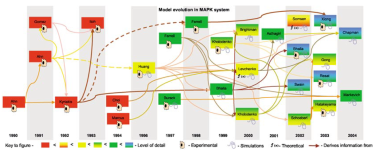
\includegraphics[width=0.8\textwidth]{img/cap_1/model_evolution.png}
    \caption{\footnotesize{Evolución del modelado de la cascada de MAPK. De izquierda a derecha el año en que se introdujo el modelo, y cada modelo se haya en una caja cuyo color representa su nivel de detalle. Éste nivel puede ir desde una mera descripción de las partes y las influencias entre ellas (como los casos rojos), a modelos simples con parámetros de prueba que demuestran comportamientos emergentes (cuadros amarillos), y hasta modelos en donde la dinámica de las interacciones esta cuantificada y existe un correlato experimental de la mecánica del modelo (cuadros azules y verdes). Debajo de cada modelo se detalla que tipo de modelado se usó y las flechas conectan fuentes de información utilizadas. Imagen tomada de \cite{Vayttaden2004}.}}
    \label{fig:evolucion_modelos}
\end{figure}

Al obtener más detalles sobre el tipo de interacciones entre especies, se llega a modelos de sistemas en los que es posible identificar motivos repetidos \citep{Tyson2003}. Aunque algunas redes pequeñas fueron delineadas con un elevado nivel de detalle, se estima que por ejemplo existen como mínimo unas 150000 interacciones proteicas en humanos, y para estudiarlas es necesario implementar técnicas de alto rendimiento \citep{Han2008}. Entre estas técnicas se encuentran inmunoprecipitación de cromatina seguido de identificación por microarray (ChIP-chip) o secuenciación (ChIP-seq) para interacciones entre factores de transcripción y genes, o purificación de co-afinidad seguido de identificación por espectroscopia de masa para interacciones entre proteínas. Por ejemplo, \cite{Soderberg2008} desarrollaron un protocolo para realizar ensayos de ligadura de proximidad \textit{in situ} y así determinar en qué compartimientos ocurren dichas interacciones. \cite{Berggard2007} confeccionaron un resumen de distintas técnicas para marcar qué proteínas interactúan entre sí. En el caso de \cite{Kang2020}, en donde utilizan inmunoprecipitación de cromatina para identificar interacciones entre factores de transcripción y ADN. Cuando la cantidad de especies e interacciones es elevada, es común hallar implementaciones de redes bayesianas donde se perturban las concentraciones de varias especies y se analizan los efectos sobre otras, como muestran \cite{Xu2010} y \cite{Sachs2005}. \cite{Mootha2003} logran asociar el origen de la deficiencia de citocromo C oxidasa a un gen a través de integración de datos de co-expresión genética, proteómica y un mapa físico de loci candidatos a enfermedad. Estos métodos permiten reconstruir las redes biológicas cuya dinámica posteriormente se interroga para generar modelos bioquímicos.

Los modelos de bioquímica celular en general se basan en la ley de acción de masas para describir las reacciones químicas. Estos pueden estar basados en diversos formalismos matemáticos, desde lógica booleana hasta ecuaciones diferenciales ordinarias. A través de la ley de acción de masas, las variaciones en las concentraciones de cada especie se pueden predecir cuantitativamente a partir de las constantes de reacción que describen sus interacciones, incluso entre distintas escalas \citep{Krakauer2011}. Agregar dichas constantes permite desarrollar modelos numéricos que pueden ser matemáticamente integrados. En el trabajo de \cite{Huang1996} se utilizan las descripciones previas de la cascada de MAPK para generar un modelo matemático simple con parámetros de prueba y demostrar un comportamiento emergente de la red en el que ésta responde fuertemente a la señal de estímulo una vez superada cierta concentración crítica, denominado ultrasensibilidad (ver \cref{fig:evolucion_modelos} cuadros amarillos).

Es común hallar en la literatura que a medida que se realizan nuevos experimentos se modifican o confeccionan modelos que describan dichos resultados, sin verificar si se mantienen predicciones previas. Idealmente se deberían agregar datos de experimentos previos y los nuevos experimentos servirían para, iterativamente, evaluar y refinar el modelo. Además, integrar modelos que contienen especies en común representa un avance en el desarrollo de modelos más completos, e incluso, modelos de célula completa como sugieren \cite{Karr2015}. Sin embargo, no siempre es posible agregar datos entre sí ya que no hay herramientas desarrolladas para tal propósito. La falta de acceso a algunos modelos, su incompatibilidad entre ellos, errores de formato o insuficiente información sobre como implementarlos son algunos de los inconvenientes usuales mencionados por \cite{Szigeti2018} a la hora de transferir modelos dentro de la comunidad.

Con el objetivo de combatir las dificultades en la transferencia de modelos, año a año se desarrollan nuevas herramientas que permiten publicar y compartir modelos, facilitando así su evaluación y refinamiento. En el trabajo de \cite{Hucka2003}, se presenta un lenguaje basado en XML, \ening{Systems Biology Markup Language} (SBML), que es utilizado para representar e intercambiar modelos de redes bioquímicas. Modelos descriptos en dicho lenguaje pueden ser subidos a distintos repositorios públicos, como el presentado por \cite{Malik-Sheriff2018}, denominado \ening{BioModels}. Bionetgen (BNGL), otro lenguaje de modelado, se basa en definir reglas de interacción entre especies, permitiendo definir en pocas líneas cómo ensamblar un polímero a partir de monómeros \citep{Harris2016}.

Asimismo, los modelos de ecuaciones diferenciales ordinarias suelen basarse en la ley de acción de masas donde las velocidades de reacción son proporcionales a las concentraciones de los reactivos \citep{Sorger2011}. Esta cinética de acción de masas es una aproximación continua a una descripción más fundamental, discreta y estocástica, que es la ecuación maestra. Como hipótesis se asume que los reactivos se encuentran bien mezclados y que el sistema se halla en equilibrio termodinámico, pero no necesariamente en equilibrio químico \citep{Chen2010}. \cite{Bhalla2002} analiza mediante estos métodos \textit{in silico} cómo la cascada de señalización de MAPK regula la sensibilidad al ligando por medio de una retroalimentación positiva entre la fosfatasa de MAPK y la proteína quinasa C (PKC) (ver \cref{fig:evolucion_modelos} cuadros azules). La dimensión espacial tiene diversos efectos sobre el sistema que pueden ser agregados utilizando ecuaciones en derivadas parciales. Este tipo de ecuaciones representan sistemas bioquímicos en tiempo y espacio continuos y modelan fenómenos de difusión, gradientes de concentración y transporte \citep{Sorger2011}. Los mismos fueron aplicados por \cite{Rehm2009} para modelar las ondas espaciales de permeabilización de membrana mitocondrial externa, encontrando y explicando por qué células hijas inician la apoptosis de forma sincrónica.

Por otro lado, el enfoque estocástico trata la evolución temporal de las variables dinámicas del sistema de forma discreta y análoga a las caminatas al azar. Considerando el carácter aleatorio que tienen las colisiones moleculares en las reacciones químicas, se utiliza una ecuación que describe la probabilidad de variación de la variable dinámica. A continuación se generan números aleatorios siguiendo las probabilidades calculadas o utilizando el método de Monte Carlo, simulando así la variable deseada \citep{Gillespie1977}. Como muestra \cite{Gillespie1977}, estos métodos pueden reproducir los resultados que provee una ecuación maestra para concentraciones homogéneas, además de proveer información valiosa sobre las fluctuaciones de la variable analizada. El modelo teórico de \cite{Friedman2006} logra reconciliar la variación temporal con las mediciones realizadas en una población celular basándose en el mecanismo de producción de proteínas subyacente. Por último, cabe destacar que las fluctuaciones de las reacciones son del orden de $1/\sqrt{N}$, siendo $N$ la cantidad de moléculas disponibles para reaccionar. Luego, si $N>10^2$ podemos usar un modelo determinista continuo despreciando estas fluctuaciones \citep{Chen2010}.

% A través de la ley de acción de masas, las variaciones en las concentraciones de cada especie se pueden predecir cuantitativamente a partir de las constantes de reacción que describen sus interacciones y entre las distintas escalas \citep{Krakauer2011}. Al agregar dichas constantes podemos desarrollar modelos numéricos que pueden ser matemáticamente integrados. Esta evolución de modelos se encuentra ejemplificada en el trabajo de \cite{Vayttaden2004} para el caso de la vía de proteínas quinasas activadas por mitógenos (MAPK, ver \cref{fig:evolucion_modelos}). \cite{Bhalla2002} analizan mediante metodos \textit{in silico} como la cascada de señalizacón de MAPk regulan la sensibilidad al ligando por medio de una retroalimentación positiva entre la fosfatas de MAPK y la proteín quinasa C (PKC).

Analicemos a forma de ejemplo el operón lactosa de \textit{escherichia coli}: la alolactosa puede unirse al represor de lactosa quien, a su vez, interactúa fuertemente con el ADN evitando que ARN polimerasas puedan acceder para transcribir ciertos genes. Cuando se alcanza cierta concentración crítica de alolactosa, ésta se une al represor haciendo que se desligue del ADN y permitiendo la síntesis del operón que codifica, entre otras proteínas, para una permeasa que permite el ingreso a la célula de más alolactosa. Cabe destacar que éste es un sistema autocatalítico ya que, una vez que se sintetizó permeasa, más alolactosa entra a la célula estimulando la síntesis de más permeasa \citep{Laurent1999}. Este tipo de red de interacciones se repite frecuentemente en sistemas biológicos ya que genera un comportamiento de tipo interruptor en respuesta a alguna variable (ver \cref{fig:switch}).

\begin{figure}
    \centering
    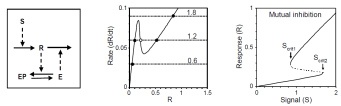
\includegraphics[width=0.8\textwidth]{img/cap_1/switch_example.png}
    \caption{\footnotesize{A la izquierda se puede ver un diagrama de las interacciones entre las especies en donde S representa alguna señal, R la respuesta del sistema y E es una especia que interactúa con R. En el ejemplo del operón de lactosa: S representa la alolactosa, R la permeasa y E el inhibidor. En el medio se grafica el cambio de concentración de la respuesta respecto al tiempo en función de R. A la derecha se muestra el diagrama de fases de la respuesta en función de la señal. Imagen tomada de \cite{Tyson2003}.}}
    \label{fig:switch}
\end{figure}

Debemos destacar en el modelo presentado anteriormente que las escalas temporales de las reacciones pueden diferir en varios ordenes de magnitud. En particular, el cambio conformacional del represor al unirse a alolactosa puede ser del orden de segundos mientras que el tiempo que tarda en sintetizarse o degradarse la permeasa está en el orden de horas. Además, las especies pueden representar distintas variantes de proteínas o complejos. En señalización intracelular suele ocurrir que el cambio que se propaga a través de la red son modificaciones postraduccionales, como fosforilaciones en sitios específicos de cada proteína y ocurren en el orden de minutos. Dependiendo el nivel de detalle del modelo, es posible tomar aproximaciones sobre distintas escalas temporales o incluso agrupar especies o reacciones en una sola.

Sistemas como el operón lactosa se hallan inmersos en una red más amplia y compleja dentro del organismo. Adicionalmente, en organismos más evolucionados, éstas redes suelen ser más grandes. Al incluir más especies con sus respectivas interacciones en un modelo, éste aumenta en complejidad. Entre las complicaciones del diseño de modelos se encuentran la dificultad de poder interpretarlos intuitivamente cuando se tienen muchos motivos interconectados y la extensión del espacio de parámetros \citep{Tyson2020}.

Separar el modelo en distintos módulos, cuando es posible, facilita tanto la interpretación de éste como la determinación de qué especies observar o perturbar  experimentalmente. Como muestran \cite{Harrington2008}, para estudiar la cascada apoptótica combinan las vías extrínseca e intrínseca mediante la implementación de módulos funcionales y subredes ya descriptas en la bibliografía para modelarla y además determinar su dinámica. Por otro lado, el análisis de respuesta modular (\ening{Modular Response Analysis}, MRA) consiste en separar la red en módulos de forma tal que solo hayan algunas especies que sirvan de mediadoras entre módulos. El desarrollo de dicho método y su aplicación a la cascada de MAPK y la regulación de asimilación de amonio en \textit{escherichia coli} fue introducido por \cite{Bruggeman2002}. En el trabajo de \cite{Santos2007}, se utiliza MRA para distinguir las diferencias en respuesta de la cascada MAPK ante estímulos distintos (ver \cref{fig:mra_ejemplo}). Aplicándolo descubren cómo al utilizar factor de crecimiento nervioso (NGF) aparece un lazo de retroalimentación positivo en lugar de uno negativo, como cuando se utiliza factor de crecimiento epidérmico (EGF). Estos tipos de análisis permiten reconstruir los comportamientos emergentes de la interacción entre distintos módulos de una red extensa.

\begin{figure}
    \centering
    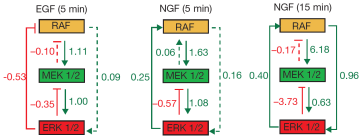
\includegraphics[width=0.6\textwidth]{img/cap_1/mra_example.pdf}
    \caption{\footnotesize{Resultados del análisis de MRA aplicado al estudio de la cascada de MAPK al utilizar dos estímulos distintos y a tiempos distintos. Imagen tomada de \cite{Santos2007}.}}
    \label{fig:mra_ejemplo}
\end{figure}

En todo tipo de modelado existe un equilibrio que debe encontrarse entre el nivel de detalle buscado y la complejidad inherente de su análisis. Modelos que consideran gran cantidad de variables e interacciones pueden ser muy detallistas y precisos, pero son más difíciles de ajustar experimentalmente, considerando la cantidad de constantes de reacción y condiciones iniciales que deben determinarse \citep{Sorger2011}. Cada interacción incluida en un modelo agrega los parámetros correspondientes a sus constantes cinéticas, mientras que cada especie va a traer aparejada su concentración inicial. Aunque algunos de estos parámetros refieren a especies intermedias cuya concentración inicial es cero, otros parámetros pueden ser muy variables en una población celular, como se aprecia en el trabajo de \cite{Spencer2009}, donde las concentraciones iniciales del modelo son tomadas aleatoriamente de una distribución lognormal. Por otro lado, en algunos casos hay más de una combinación de parámetros que reproducen soluciones indistinguibles desde un punto de vista experimental. Aunque se invierte mucho esfuerzo en determinar los parámetros para los modelos, algunos trabajos destacan la importancia de identificar adecuadamente la topología de la red en lugar de la mejor combinación de parámetros. \cite{Frohlich2018} desarrolla un método para acelerar considerablemente las simulaciones de sus modelos, y así realizar un análisis más exhaustivo de cómo la variación en los parámetros afecta la incertidumbre de ciertos observables. Por otro lado, en el trabajo de \cite{Santolini2018} se afirma que un 65\%-80\% de la precisión de los modelos depende de encontrar adecuadamente la topografía de la red, y lo remanente a determinar correctamente los parámetros. A modo de ejemplo, \cite{Kraeutler2010} estudian la señalización $\beta$-adrenérgica de los cardiocitos modelándola mediante ecuaciones de Hill para las interacciones y muestran que pueden recuperar comportamientos clave sin necesidad de ajustar todos los parámetros.


%%%%%%%%%%%%%%%%%%%%%%%%%%%%%%%%%%%%%%%%
\section{Cómo interrogar la dinámica de redes biológicas}


Para interrogar redes biológicas resulta importante ser capaz de reportar la dinámica de actividad de distintos nodos de la red simultáneamente y a nivel de célula única debido a su inherente variabilidad. Durante los últimos tiempos, hubo una explosión en el desarrollo de biosensores genéticamente codificados que permitió cuantificar la actividad de diversas enzimas como proteína G acoplada a receptor (GPCR, ver \cref{fig:pthr}), quinasa regulada por señalización extracelular (ERK), quinasa c-Jun N-terminal (JNK), entre muchas otras, así como la presencia de moléculas pequeñas \citep{Greenwald2018}.

\begin{figure}
    \centering
    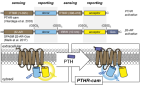
\includegraphics[width=0.65\textwidth]{img/cap_1/pthr.pdf}
    \caption{\footnotesize{Esquema de un sensor de un tipo de receptor asociado a proteína G llamado PTHR. Éste consiste en el receptor modificado para incluir a CFP como donante y YFP como aceptor. En su configuración basal, los fluoróforos se encuentran suficientemente cerca como para transferir energía por FRET de CFP a YFP, sin embargo, el cambio conformacional producido por la unión del ligando, PTH, aleja los fluoróforos entre sí, interrumpiendo dicha transferencia. Analizar el ratio de intensidad de emisión entre los canales cian y amarillo permitirá determinar el estado de la población de receptores. Imagen tomada de \cite{Greenwald2018}.}}
    \label{fig:pthr}
\end{figure}

El mecanismo de funcionamiento de estos reporteros consiste en diseñarlos de forma tal que sus propiedades espectroscópicas sean sensibles al entorno \citep{Bastiaens1999}. Mientras algunos de estos sensores no emiten fluorescencia en uno de estos estados, otros hacen uso de dos moléculas fluorescentes y la capacidad de intercambiar energía entre ellas a través de un proceso denominado Transferencia de Energía de Resonancia de Förster (FRET). Dicho fenómeno consiste en la transferencia de energía entre un fluoróforo y otro de manera no radiativa como resultado de un acoplamiento dipolo-dipolo. Para que esto ocurra, se deben dar varias condiciones: que la distancia entre ambos sea del orden de 5~nm, sus orientaciones lo permitan y que el espectro de emisión del donante se superponga con el de excitación del aceptor. Cabe recalcar que los biosensores basados en FRET se pueden clasificar en heteroFRET, si las especies de fluoróforos utilizados son distintos, u homoFRET, cuando son idénticos.

Los biosensores basados en heteroFRET son más ubicuos y, para estimar la eficiencia de FRET, se procede a excitar al dador y luego cuantificar la intensidad de la emisión del dador y aceptor en sus respectivos canales. \cite{Miyawaki1997} presentan en su trabajo un sensor basado en CFP y YFP conectados por calmodulina y un péptido M13 que se unen de forma reversible al ion de calcio (ver \cref{fig:bios}A). Dicho biosensor fue utilizado para estimar las concentraciones de calcio en distintos compartimientos celulares. Por otro lado, \cite{Grashoff2010} desarrollaron un biosensor compuesto por los fluoróforos mTFP1 y Venus, unidos por un segmento elástico, que fue utilizado para medir fuerzas entre proteínas. Una vez calibrados, este tipo de sensores permiten transducir eficiencia de FRET en tensión sensada y así estudiar la evolución de las fuerzas entre proteínas en adhesiones focales (ver \cref{fig:bios}B). La posibilidad de implementar este tipo de biosensores en células y organismos vivos permite obtener información sobre la temporalidad y espacialidad de distintas redes biológicas.

\begin{figure}[htb]
    \centering
    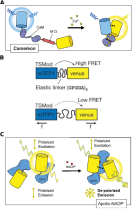
\includegraphics[width=0.5\textwidth]{img/cap_1/biosensors.pdf}
    \caption{\footnotesize{\textbf{A.} Esquema de un biosensor de calcio basado en heteroFRET y compuesto por CFP y YFP, unidos por calmodulina y un péptido M13. Imagen tomada de \cite{Greenwald2018}. \textbf{B.} Esquema de un sensor de fuerzas moleculares compuesto por mTFP1 y Venus, unidos por una secuencia elástica. Imagen tomada de \cite{Grashoff2010}. \textbf{C.} Esquema de un biosensor basado en homoFRET y capaz de sensar la presencia de NADPH en las células. Imagen tomada de \cite{Greenwald2018}.}}
    \label{fig:bios}
\end{figure}

En el caso de los biosensores basados en homoFRET, en lugar de utilizar distintos canales de emisión para analizar la eficiencia de FRET, se utiliza microscopía de anisotropía de polarización. Considerando que el eje de excitación de las proteínas fluorescentes es casi paralelo al de emisión y dado que el tiempo de vida de fluorescencia en citoplasma ($\sim2.6$~ns) es considerablemente menor que el tiempo de correlación rotacional ($\sim36$~ns), ésta microscopía consiste en excitar la muestra con luz polarizada para realizar una fotoselección y luego analizar la anisotropía de fluorescencia, estudiando la emisión en la polarización paralela y perpendicular a la excitación  \citep{Swaminathan1997}. Si los fluoróforos fotoseleccionados son monoméricos tendrán una emisión anisótropa, mientras que si se encuentran en estado dimérico la emisión será más isótropa ya que por FRET parte de la emisión será en el eje del fluoróforo aceptor que no se encuentra necesariamente paralelo al donante. \cite{Cameron2016} desarrollaron Apollo, un biosensor basado en homoFRET para sensar el estado redox de la célula y muestran como NADPH se depleta en células $\beta$ previo a la acumulación de peróxido de hidrógeno (ver \cref{fig:bios}C). Una gran ventaja de utilizar este tipo de biosensores es que tienen un ancho espectral mucho menor y no es necesario utilizar dos canales distintos para observar el dador y el emisor, permitiendo multiplexar señales de más biosensores, como muestran \cite{Warren2015} al combinar un sensor de heteroFRET para calcio y uno de homoFRET para cúmulos de fosfatidilinostol.

% Estudiar la orientación del fluoróforo unido a la cabeza de myosina (S$_1$) permitió identificar su disposición y orientación al unirse a F-actina. En el trabajo de \cite{Andreev1993}, se concluyó que S$_1$ podía unirse de dos formas distintas según se halle en exceso o déficit en relación a la cantidad de F-actina. Conociendo el efecto que tiene la viscosidad del medio sobre el tiempo de correlación de rotación del fluoróforo, la anisotropía de fluorescencia puede ser utilizada para obtener información sobre parámetros reológicos del citosol, como se muestra en el trabajo de \cite{Swaminathan1997}. Por otro lado, dado que la unión del fluoróforo a otra molécula produce un cambio en la anisotropía, se la puede utilizar para reportar la proporción de fluoróforos ligados entre el total de fluoróforos. \cite{Dubach2014} utilizan esta técnica \textit{in vivo} para observar la dinámica de interacción entre la droga y su blanco (Olaparib) en tiempo real, mostrando su utilidad para descifrar la dinámica intracelular.

Tradicionalmente, los estudios de las interacciones involucradas en señalización dependían de análisis \textit{in vitro} como Western Blot o ensayos enzimáticos. En el caso de los Western Blots, se somete a una población celular a un tratamiento particular y luego se procede a lisar y recuperar el contenido intracelular de la población, del compartimiento de interés, y cuantificarlo. Éstos métodos continúan siendo importantes para determinar las interacciones entre especies, pero las ventajas introducidas por los biosensores fluorescentes genéticamente codificados los hace cruciales para estudiar la dinámica temporal de las señales. \cite{Ryu2015} retoman el estudio de como células PC12 responden de forma distinta ante EGF y NGF, y mediante la implementación de EKAR, un biosensor basado en heteroFRET que cambia su conformación al ser fosforilado en una subunidad de ERK, encuentran que el tipo de respuesta se encuentra codificado en la frecuencia de la señalización (ver \cref{fig:dinamica_temporal}A). Es fácil ver que si el sistema en estudio presenta oscilaciones, cualquier técnica que promedie en una población celular o carezca de información temporal, no será útil para estudiarlas. Con esto en mente, \cite{Barbosa1998} utilizan Fura-2 para relacionar las oscilaciones de Calcio intracelular en células $\beta$ generadas por niveles elevados de glucosa extracelular y la subsecuente liberación pulsada de insulina (ver \cref{fig:dinamica_temporal}B). \cite{Fosbrink2010} desarrollan el biosensor JNKAR1 para estudiar la como la vía JNK integra señales de supervivencia o muerte celular. Éste biosensor esta basado en heteroFRET y aumenta 15 a 30\% el ratio de emisión de amarillo a cyan una vez fosforilado. Por medio de dicho biosensor sientan las bases de la dinámica de la cascada JNK demostrando la rapidez con que se propaga la señal dentro de la célula, su carácter biestable, ultrasensible y bimodal ante estímulos ribotóxicos como anisomicina (ver \cref{fig:dinamica_temporal}C).

\begin{figure}
    \centering
    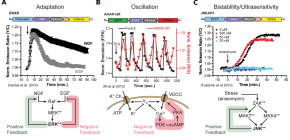
\includegraphics[width=0.9\textwidth]{img/cap_1/dinamica_temporal.pdf}
    \caption{\footnotesize{Mediciones de la dinámica temporal de distintos biosensores que ponen en evidencia comportamientos emergentes de redes biológicas. Imagen tomada de \cite{Greenwald2018}. \textbf{A.} Dinámica temporal de una respuesta adaptativa. En este caso, aunque ambos metabolitos comparten la vía de señalización, debido a diferencias en la frecuencia del estímulo, se producen respuestas distintas a nivel celular. \textbf{B.} Multiplexar la dinámica oscilatoria del Calcio intracelular permite encontrar cómo ésta se halla regulada por distintas vías. \textbf{C.} Estudiar la dinámica del reportero de actividad de JNK permite describir el comportamiento ultrasensible y biestable de la vía JNK al estrés.}}
    \label{fig:dinamica_temporal}
\end{figure}

Visualizar la dinámica mediante biosensores no solo resulta beneficioso para ver la temporalidad, sino también la variabilidad intercelular. Las oscilaciones mencionadas previamente suelen ser asincrónicas por lo que solo es posible estudiarlas si observamos a nivel de célula única. \cite{Aoki2013} demostraron a través de EKAREV, un biosensor de ERK, que pulsos de actividad en células individuales tienen un efecto paracrino sobre las células vecinas y sirven para controlar la proliferación. Incluso cuando el proceso bajo estudio puede ser sincronizado, como es el caso del ciclo celular, la variabilidad intercelular hace que las células se desfasen entre sí, dificultando su análisis.

Dada la elevada interconectividad de las redes biológicas y considerando su variabilidad, resulta crucial poder multiplexar varios nodos, es decir, observar su actividad simultáneamente. Muchas de las técnicas son discutidas por \cite{Grecco2016}. Algunas estrategias consisten en observar biosensores diferentes expresados en células distintas y relacionarlos a través de un marcador de referencia como el llamado ``multiplexado computacional''. Por ejemplo, \cite{Machacek2009} relacionan la señal obtenida de sensores para Rac1, Cdc42 y RhoA con la protrusión celular utilizando lo que se denomina multiplexado computacional. El limitante físico en la cantidad de biosensores que pueden ser visualizados en el mismo espacio está dado por el espectro disponible. Por esta razón, biosensores con espectros reducidos como los basados en homoFRET o en aplacamiento (quenching) resultan ideales. \cite{Mehta2018b} demuestran que es posible utilizar hasta seis biosensores simultáneamente, mientras sea posible confinar algunos de ellos a ciertos compartimentos subcelulares.


%%%%%%%%%%%%%%%%%%%%%%%%%%%%%%%%%%%%%%%%
\section{La red de caspasas como modelo}
\label{sec:intro:CascadaApoptotica}


%Existen numerosos modelos en los repositorios presentados en la sección \ref{sec:intro:EstudiarRedes}. Muchos de estos fueron preparados para describir el comportamiento de alguna red en un contexto específico. Debido a la carencia teórica de como combinar modelos en uno solo conservando las propiedades previas y la dificultad de agregar datos o experimentos en un solo paquete, muchos de estos modelos describen el comportamiento de distintos módulos de redes biológicas sin poder ser combinados entre sí o extrapolados a distintas situaciones. La cascada apoptótica es un claro ejemplo de esto ya que esta compuesta por varios módulos y, considerando que puede ser iniciada por distintos tipos de estímulos, la dinámica puede depender del desencadenante.

La apoptosis es un proceso de muerte celular programada que ocurre en organismos multicelulares de forma ordenada, sin liberar el contenido intracelular al espacio intercelular, evitando así dañar a las células vecinas. Para tomar esta decisión, las células integran información sobre el entorno en el que se hallan, así cómo cuánto daño celular interno acumulado contienen. Este programa juega un rol fundamental tanto durante el desarrollo embriológico de órganos, como para el mantenimiento del número de células, entre otras cosas. Es un proceso finamente regulado que cuando se altera produce graves patologías como malformaciones o aparición de tumores, así como también enfermedades neurodegenerativas por citar algunos ejemplos \citep{Kominami2012}. Contrariamente, la necrosis es un proceso de muerte desordenado que genera una serie de reacciones locales, conduciendo a respuestas de tipo inflamatorio. Entender el mecanismo de inducción de apoptosis, sin generar elevados niveles de necrosis, es importante en la generación de tratamientos para enfermedades como el cáncer.

Desde un punto de vista evolutivo, ésta cascada está muy bien conservada y los engranajes principales de la maquinaria apoptótica son las caspasas \citep{Sakamaki2009}. Estas pertenecen a una familia de proteínas denominado cisteín-proteasas y se encargan de clivar proteínas reconociendo una secuencia específica de aminoácidos. En circunstancias normales, las caspasas se hallan expresadas constitutivamente en su forma inactiva como zymógenos o procaspasas. Para gatillar la cascada de caspasas que desencadena la apoptosis se pueden estimular dos vías diferentes, intrínseca y extrínseca, que producen dinámicas distintas en el sistema. La vía intrínseca surge de señales provenientes de adentro de la célula, como estrés celular o daño al ADN, mientras que, la vía extrínseca es desencadenada por estimulación de receptores de membrana celular llamados receptores de la muerte \citep{Kominami2012a}. Su activación se encuentra regulada en numerosos puntos, siendo necesario por lo tanto una cascada de eventos para que la célula se vea irreversiblemente determinada a la apoptosis. Es posible disecar la cascada en los módulos que la componen que son el extrínseco, encargado de transducir señales extracelulares y dar inicio al proceso, el intrínseco, que inicia la cascada en respuesta a daño celular, y el efector, en el que convergen ambos módulos iniciadores para la completa ejecución del proceso (ver \cref{fig:Sketch}).

\begin{figure}
    \centering
    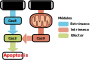
\includegraphics[width=0.5\textwidth]{img/cap_1/flujo_sketch.pdf}
    \caption{\footnotesize{Esquema del flujo de la señal en la cascada apoptótica. Ésta puede ser desencadenada por estímulos intrínsecos o extrínsecos y la señal luego converge en el módulo efector. Adaptado de \cite{Corbat2021}.}}
    \label{fig:Sketch}
\end{figure}

Los distintos módulos de la cascada apoptótica así cómo la dinámica al iniciarla a través de dos tipos de estímulo distintos fueron analizados por separado o en distintas combinaciones entre sí. Por ejemplo, \cite{Bentele2004} se concentran en analizar la respuesta de la red ante estímulos extrínsecos y cual es la sensibilidad de la dinámica ante una perturbación en cada parámetro. Por otro lado, \cite{Rehm2006} incluyen en su modelo solo los módulos intrínseco y efector y determinan la importancia de los lazos de retroalimentación en la red para superar las inhibiciones del sistema. Análogamente, \cite{Legewie2006} también analizan las vías intrínseca y efectora para recalcar la importancia de los lazos de retroalimentación positiva para generar biestabilidad en el sistema.

\begin{figure}
    \centering
    \includegraphics[width=0.8\textwidth]{img/cap_1/ModeloCompleto.png}
    \caption{\footnotesize{Esquema del modelo completo de la cascada apoptótica desarrollado por  \cite{Albeck2008}. Se pueden apreciar en colores distintos los módulos incluidos en el modelo, así como distintos compartimientos. Imagen tomada de \cite{Albeck2008}.}}
    \label{fig:ModeloCompleto}
\end{figure}

Uno de los modelos más completos de la cascada apoptótica es \ening{Extrinsic Apoptotic Reaction Model} (EARM). Éste fue desarrollado por \cite{Albeck2008} con el objetivo de describir dos características clave de la red: la variabilidad en el desencadenamiento de la cascada y la instantaneidad una vez iniciado el proceso. Para desarrollar dicho modelo, el grupo utilizó sensores basados en heteroFRET para estudiar la dinámica de la caspasa 8, iniciadora de la vía extrínseca, y la caspasa 3, efectora, en distintos experimentos perturbativos utilizando ARN de interferencia para bloquear la transducción de ciertas especies. Dicho modelo cuenta con 58 especies que corresponden a 18 moléculas cuyas condiciones iniciales son distintas de 0 y 40 especies adicionales que representan complejos, proteínas clivadas, o formas localizadas de especies iniciales que interactúan mediante 28 reacciones con 70 constantes de reacción que son no nulas (ver \cref{fig:ModeloCompleto}).

EARM se divide en cuatro módulos. El primero (gris) consiste en una representación agrupada de la unión del factor de necrosis tumoral (TNF por sus siglas en inglés) o ligando de inducción de apoptosis relacionado con TNF (TRAIL por sus siglas en inglés) al receptor y la subsecuente activación de la procaspasa 8 mediante el complejo de señalización de inducción de muerte (DISC por sus siglas en inglés) unido al receptor. En segundo lugar (azul), se muestra la cascada enzimática en que la caspasa 8 activa cliva a la procaspasa 3, la cual a su vez cliva otros sustratos efectores. Por otro lado, se muestra la vía mitocondrial (amarillo) por la cual la caspasa 8 activa trunca a Bid para dar lugar a la activación de Bax que luego dará lugar a la formación de poros en la membrana mitocondrial por los cuales citocromo C (CyC por sus siglas en inglés) y Smac son traslocados al citosol; una vez ahí, se forma el apoptosoma a partir de Apaf-1 y procaspasa 9, para clivar y activar aún más moléculas de caspasa 3. Por último, se representa (verde) un lazo de retroalimentación positivo entre la caspasa 3 y la procaspasa 8 mediado por la caspasa 6, que es clivada y activada por la caspasa 3.

Sumado a las aproximaciones implícitas en ley de acción de masas, la construcción de este modelo agrega otras tres aproximaciones que deben tenerse en cuenta. En primer lugar, la formación de DISC y el apoptosoma que incluyen unión de varias proteínas fue simplificado usando una representación con parámetros agrupados. En segundo lugar, se omitió la síntesis y degradación de cualquier proteína (exceptuando la degradación de caspasa 3 una vez unida a XIAP). Por último, especies con actividades similares fueron representadas por una única especie, entre ellas están: caspasa 8 y caspasa 10, caspasa 3 y caspasa 7 y la familia de proteínas similares a Bcl-2.

Por otro lado, \cite{Zhang2009} hacen un análisis modular de la cascada apoptótica intrínsecamente estimulada. En su trabajo, dividen la cascada en: un módulo iniciador que integra señales provenientes del sensado de daño genético (relacionado principalmente con p53) que culmina con la activación BAX; un módulo amplificador que inicia con BAX formando poros en la membrana mitocondrial y rápidamente liberando el contenido mitocondrial al citoplasma; y el módulo ejecutor que incluye la formación y activación del apoptosoma y la caspasa intrínseca, así como la caspasa efectora. Cabe destacar que la rápida liberación del contenido mitocondrial se condice con los resultados observados y descriptos por \cite{Albeck2008}.

Entre los biosensores basados en FRET se encuentra un grupo capaz de sensar actividad de proteasas. Estos consisten en dos fluoróforos unidos por una secuencia sensible a la actividad de la proteasa en estudio. Las propiedades espectroscópicas de los fluoróforos seleccionados son tales que, cuando el biosensor se halla en estado dimérico, ocurra una transferencia de energía por resonancia de Förster entre ellos. Así, cuantificando dicha transferencia de energía, es posible estimar la proporción de biosensores en estado dimérico o monomérico \citep{Greenwald2018}. En los trabajos de \cite{Tyas2000} y \cite{Rehm2002} utilizan fluoróforos cyan y amarillos unidos por la secuencia DEVD, reconocida por la caspasa efectora, para mostrar que la actividad de la caspasa ocurre rápidamente en un intervalo de tiempo reducido (del orden de 15 minutos), mientras que el instante en el que ocurre es mucho más variable (del orden de horas) y depende de otros factores como tipo celular, droga y concentración usadas, entre otros. Dentro del grupo, \cite{Stegemann2015} utilizan un biosensor basado en homoFRET que consiste en dos fluoróforos de mCitrine unidos por la secuencia DEVD y cuyo estado puede analizarse mediante microscopía de anisotropía en polarización. En el trabajo analizan la dinámica de apoptosis al utilizar substratos fotoinducibles, disueltos o fijos en superficies, que generan especies reactivas del oxígeno. Cabe destacar que, aunque el sustrato disuelto genera elevados niveles de muerte celular, cuando se encuentra fijo a una superficie, actúa como factor protector (ver \cref{fig:stegemann}).

\begin{figure}
    \centering
    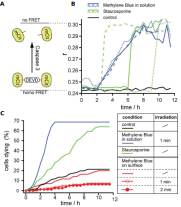
\includegraphics[width=0.6\textwidth]{img/cap_1/stegemann.pdf}
    \caption{\footnotesize{\textbf{A.} Descripción esquemática del biosensor de caspasa 3 basado en homoFRET. \textbf{B.} Curvas de anisotropía correspondientes al biosensor de caspasa 3 transfectado en células que fueron sujetas a tratamientos con staurosporina o azul de metileno. \textbf{C.} Porcentaje de células que sobreviven ante tratamientos con staurosporina o azul de metileno en solución o las superficies funcionalizadas con azul de metileno y luego fotoinducidas. Es interesante notar que las células expuestas a azul de metileno disuelto e irradiadas muestran un elevado porcentaje de muerte celular mientras que las que fueron expuestas a superficies funcionalizadas con azul de metileno e irradiadas muestran menor muerte celular que el caso control.  Imagen tomada de \cite{Stegemann2015}.}}
    \label{fig:stegemann}
\end{figure}

En conclusión, la red de caspasas es ideal para poner a punto diversas metodologías para estudiar y simular redes biológicas. Cada uno de los módulos de la cascada apoptótica tiene una caspasa cuya actividad de proteasa puede ser observada a través de biosensores análogos a los previamente descriptos. Además, la cantidad de estos módulos es suficiente como para poder multiplexarlos a nivel de célula única por medio de biosensores basados en homoFRET. Por último, la extensa librería de modelos describiendo partes o la totalidad de la red brinda un buen punto de partida y los variados experimentos caracterizando distintos comportamientos de la red dan cuenta de los comportamientos que deben emerger del modelo.


%%%%%%%%%%%%%%%%%%%%%%%%%%%%%%%%%%%%%%%%
\section{Esquema de la Tesis}

El objetivo de este trabajo fue generar un modelo matemático para describir la dinámica de la red de caspasas en distintos contextos biológicos. Tener una visión más integrada de la red será útil para comprender mejor la interconectividad entre sus módulos así como para plantear diversas soluciones terapéuticas. Además, el flujo de trabajo utilizado podría ser aplicado para el estudio de otros sistemas en dónde también se integre información.

% Para ello fue necesario confeccionar un paquete de datos que amalgame experimentos realizados en contextos distintos y cuyos observables pueden ser fácilmente comparados con predicciones del modelo. Considerando éste objetivo específico, fue necesario desarrollar e implementar un biosensor capaz de interrogar varios nodos de la red, simultáneamente y a nivel de célula única y minimizar la perturbación introducida. 

En primer lugar, en el capítulo 2 presentaré cómo realizar y analizar experimentos utilizando un sensor genérico análogo al presentado en el trabajo de \cite{Stegemann2015}. Para ello describiré un modelo mínimo utilizando uno de estos sensores, en qué consiste la microscopía de anisotropía en polarización y como analizar las imágenes obtenidas para obtener un observable robusto y comparable entre experimentos y con los resultados del modelado. El análisis desarrollado se encuentra publicado en \cite{Corbat2018}.

Luego, en el capítulo 3 describiré los biosensores basados en homoFRET utilizados para los distintos experimentos. Discutiré cómo fueron seleccionados los pares de fluoróforos, el diseño de los plásmidos utilizados y la metodología utilizada para reducir las perturbaciones que introducen en el sistema. El estudio de los distintos pares de fluoróforos se encuentra presentado en \cite{Corbat2018}, mientras que las mejoras introducidas al biosensor y el efecto de sus perturbaciones en la red se haya publicado en \cite{Habif2021}.

Finalmente, en el capítulo 4 analizaremos los resultados de distintos experimentos donde se indague la dinámica de la red apoptótica para generar un modelo integrador de todos los módulos de la red. Una vez generado dicho modelo, mostraré su capacidad predictiva ante distintos experimentos realizados previamente y así verificar que no se redujo su capacidad predictiva. Un primer modelo describiendo el comportamiento de la red ante estímulos extrínsecos se haya presentado en \cite{Corbat2018}, mientras que el modelo integrador que describe el comportamiento de la cascada ante distintos estímulos y en contextos diferentes se encuentra en \cite{Corbat2021}.


%%%%%%%%%  Materiales y Metodos
\chapter{De la Señal Fotofísica al Observable Biológico}
\label{cap:MatMet}


En este capítulo, detallaré cómo analizar experimentos de microscopía de anisotropía en polarización de un biosensor como el utilizado por el grupo previamente en el trabajo de \cite{Stegemann2015}. Comenzaré por una descripción de la microscopía de anisotropía de polarización utilizada para observar este tipo de sensores, cómo transfectarlo a las células y el protocolo de adquisición y análisis de imágenes pertinente. Finalmente, a partir de un modelo minimalista que incluya estos biosensores, desarrollaré como estimar la actividad de cada caspasa a partir de los cambios en anisotropía del biosensor correspondiente y definiré un observable robusto que sirve de referencia a la activación de la caspasa.



%%%%%%%%%%%%%%%%%%%%%%%%%%%%%%%%
\section{Microscopía de Anisotropía de Polarización}


Los fluoróforos en particular poseen momentos de transición de absorción y emisión subtendidos en direcciones específicas. Esto se traduce en que la probabilidad de excitar un fluoróforo con luz linealmente polarizada depende del ángulo entre el eje de polarización de la excitación y el momento de transición de excitación y, a su vez, la emisión será polarizada y paralela al momento de transición de emisión. La polarización de la emisión puede ser afectada por diversos factores. Para empezar, los momentos de transición de excitación y emisión no siempre son colineales. Adicionalmente, el fluoróforo excitado puede rotar libremente durante el tiempo de vida del estado excitado contribuyendo así a la depolarización. Es así que cuando el tiempo de vida del estado excitado es mayor o comparable a la escala temporal de la difusión rotacional, dichos fluoróforos se implementan en biofísica para el análisis de viscosidad del medio en el que se encuentran inmersos \citep{Lakowicz2006}.

Debido a que ambos fluoróforos que componen un biosensor basado en homoFRET son indistinguibles espectralmente (como el de \cite{Stegemann2015}), necesitaremos hacer uso de otras propiedades de la luz para determinar su estado. En este caso, utilizaremos las propiedades depolarizantes del biosensor para estimar el estado de la población. Sabiendo que en el citoplasma celular el tiempo de vida de fluorescencia es considerablemente menor que el tiempo característico de rotación para una proteína fluorescente (y aún más para un dímero), ésta no contribuirá fuertemente a la depolarización. Sin embargo, la contribución a la depolarización debido a FRET es considerable ya que los fluoróforos aceptores se encuentran alineados aleatoriamente. De está forma, la población de biosensores en estado dimérico contribuirá más fuertemente a la depolarización que aquellos en estado monomérico.

Usualmente, la anisotropía se utiliza como medida de la polarización de una muestra. La anisotropía se define matemáticamente como

\begin{equation}
    r = \frac{I_{\parallel} - I_{\perp}}{I_{\parallel} + 2 I_{\perp}}.
    %\label{eq:anisotropia}
\end{equation}

\noindent Esto se consigue experimentalmente mediante el uso de analizadores para observar la intensidad de fluorescencia emitida en el eje paralelo al de incidencia (I$_{\parallel}$), así como también en el eje perpendicular (I$_{\perp}$). Cabe destacar que se trata de una magnitud adimensional ya que está normalizada por la intensidad total de fluorescencia y, por lo tanto, es independiente de la concentración de fluoróforo presente.

La anisotropía de una muestra puede medirse tanto en cubetas como mediante microscopía. La microscopía de fluorescencia permite indagar sobre las propiedades y el comportamiento de las células de forma poco invasiva y con elevada especificidad y sensibilidad. Considerando los componentes necesarios, resulta simple adaptar un microscopio comercial para visualizar anisotropía de polarización. En primer lugar, se debe colocar un polarizador en el camino del haz de excitación. Hay más de una forma de adaptar el canal de emisión para poder visualizar ambas polarizaciones simultáneamente o secuencialmente. Utilizando cristales birefringentes como calcita, es posible separar el haz en sus dos componentes de polarizaciones perpendiculares y utilizar tanto dos detectores como regiones separadas del sensor de una única cámara. Por otro lado, si la velocidad del sistema es considerablemente mayor que la variación de anisotropía de la muestra, se pueden colocar dos analizadores cruzados en una rueda de filtros para seleccionar la polarización a ser adquirida (ver \cref{fig:esquemaAnisotropia}).

\begin{figure}
    \centering
    \includegraphics[width=0.75\textwidth]{img/cap_2/EsquemaAnisotropia.png}
    \caption{\footnotesize{Esquema de un armado experimental típico de un microscopio adaptado para ver anisotropía de polarización. Se utiliza un polarizador para que la excitación sea linealmente polarizada. El haz ingresa a la muestra y la fluorescencia es colectada a través del mismo objetivo. Se utilizan dos analizadores para observar las componentes emitidas paralela y perpendicular a la excitación.}}
    \label{fig:esquemaAnisotropia}
\end{figure}

Durante la calibración del sistema, es necesario considerar y corregir las depolarizaciones introducidas por el sistema óptico utilizado. Por ejemplo, la elevada amplitud numérica de las lentes objetivo utilizadas capturan una mezcla de polarizaciones distintas debido al cono de luz de emisión subtendido en un amplio ángulo sólido en el punto de muestreo. La calibración del factor G se utiliza para corregir las diferencias en sensibilidad del sistema para polarizaciones cruzadas. Para determinarlo, se utiliza un valor de referencia de anisotropía de un fluoróforo mediante la ecuación

\begin{equation}
    G = \frac{I_{\parallel} (1 - r_{ref})}{I_{\perp} (1 + 2r_{ref})},
\end{equation}

\noindent donde $r_{ref}$ es el valor de anisotropía conocido de la muestra. Dicho factor se utiliza en el cálculo de anisotropía siguiendo

\begin{equation}
    r = \frac{I_{\parallel} - G I_{\perp}}{I_{\parallel} + 2 G I_{\perp}}.
    % \label{eq:anisotropia}
\end{equation}

\noindent Al utilizar una referencia isótropa, como ser una muestra de fluoróforo diluido, es posible llegar a una expresión donde las intensidades paralela y perpendicular deben ser normalizadas por los valores de intensidad paralela y perpendicular medidas en la referencia. Esto tiene la doble ventaja de que al utilizar imágenes, se corrigen tanto inhomogeneidades en la iluminación como los factores depolarizantes del sistema óptico.


%%%%%%%%%%%%%%%%%%%%%%%%%%%%%%%%
\section{Diseño Experimental}


Para los experimentos descriptos en esta tesis, se utilizó un microscopio comercial invertido Olympus IX-81. Con el objetivo de adaptarlo se utilizaron tres polarizadores (Meadowlark Optics), uno de ellos en el camino de excitación, y dos de ellos en una rueda de filtros ubicada en el puerto lateral en el camino de emisión. Cabe destacar que se tuvo especial cuidado en la colocación del polarizador de excitación ya que debe estar alejado de fuentes de calor, como lo son algunas fuentes de iluminación. En este caso, la fuente de iluminación utilizada fue una MT20 de Olympus con una lámpara halógena conectada mediante fibra óptica de líquido. Se utilizó un objetivo HC PL APO 63x/1.4 NA CS2 de inmersión en aceite (Leica Microsystems). También fue utilizada una cámara Orca CCD (Hamamatsu Photonics). El software de adquisición consistió en CellR (Olympus).

El microscopio adaptado y utilizado se encuentra en el Instituto Max Planck de Fisiología Molecular de Dortmund, Alemania. Previo al inicio de la tesis doctoral, se desarrolló una rueda de filtros impresa en 3D y controlada por Arduino que actualmente es de libre acceso. Distintos modelos de estas ruedas fueron impresas para adaptar microscopios comerciales y un microscopio de iluminación de plano único (SPIM, por sus siglas en inglés) en nuestro laboratorio (\cref{fig:ruedas}).

\begin{figure}[b]
    \centering
    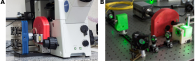
\includegraphics[width=0.9\textwidth]{img/cap_2/ruedas.pdf}
    \caption{\footnotesize{Imágenes de la rueda de filtros desarrollada en el laboratorio y montada en un microscopio comercial IX-71 (\textbf{A}) y uno de iluminación de plano único (\textbf{B}) para adaptarlos a microscopía de anisotropía de fluorescencia.}}
    \label{fig:ruedas}
\end{figure}

Las muestras consistían en células inmortalizadas de cáncer de cuello uterino (HeLa) cultivadas en pocillos de LabTek. Dado que es necesario mantenerlas viables a lo largo del experimento, las muestras se mantuvieron a 37$^{\circ}$C, 5\% de CO$_2$ y una humedad elevada $>$ 60\% mediante una cámara de cultivo y un Stable Z Specimen Warmer (Bioptechs Inc.). Dichas células fueron cultivadas en medio DMEM alto en glucosa, con 10\% de suero fetal bovino y suplementadas con 10~mg/ml de piruvato de sodio, 2~mmol/L de L-glutamina y antibióticos (100~U/mL penicilina, 100~$\mu$g/mL streptomicina) en una atmósfera humidificada, al 5\% de CO$_2$ y 37$^{\circ}$C.

Considerando que el proceso de apoptosis puede desencadenarse en cualquier momento entre el agregado de la droga estimulante y las 15 horas subsiguientes, fue necesario automatizar la adquisición de imágenes durante el experimento. Mediante una platina motorizada y el software CellR (Olympus) se programó el microscopio para adquirir imágenes secuenciales de varias posiciones de cada pocillo. En cada uno de los pocillos se colocaron distintas drogas que servían tanto de control como estímulo. Las imágenes adquiridas son posteriormente segmentadas y analizadas para generar un cuerpo de datos que contiene una curva de intensidad promedio en cada polarización y en cada célula detectada (\cref{fig:procedimiento_exp}).

\begin{figure}
    \centering
    \includegraphics[width=0.7\textwidth]{img/cap_2/ProcedimientoExperimental.pdf}
    \caption{\footnotesize{Esquema del procedimiento experimental. Este consistió en sembrar las muestras con distintas drogas en pocillos de LabTek, adquirir una imagen de cada polarización en cada tiempo, segmentar y analizar dichas imágenes y, finalmente, generar un cuerpo de datos con las curvas de intensidad promedio de cada polarización de cada célula detectada.}}  
    \label{fig:procedimiento_exp}
\end{figure}

En cuanto a los parámetros de adquisición, se tuvieron varios cuidados distintos, tanto para no afectar significativamente la viabilidad de la muestra como para adquirir imágenes de suficiente calidad. Por un lado, la potencia de la iluminación no debe ser muy elevada ni prolongada para evitar el fotodaño a las células. Por otro lado, el tiempo de adquisición debe ser suficiente para aprovechar el rango dinámico de la cámara. Es importante destacar que no se debe buscar el 100 \% del rango dinámico ya que durante el transcurso del experimento la intensidad de fluorescencia por píxel va a aumentar y podría saturar por dos razones. En primer lugar, al clivarse el biosensor, su fluorescencia en el canal paralelo aumentará. En segundo lugar, las células al entrar en apoptosis se despegan del vidrio y adquieren una forma pequeña y redondeada que concentra el fluoróforo y aumenta la intensidad por píxel. La importancia de este cuidado radica, no solo en evitar saturar la región correspondiente a la célula imposibilitando su medición, sino que por efecto de arrastre de electrones se puede afectar la adquisición de toda la tira de píxeles, arruinando así otras regiones (\cref{fig:saturacion}). En el caso del sensor utilizado por el grupo previamente, se utilizó un tiempo de exposición de 50~ms y una potencia de iluminación elevada. Esto es posible ya que el fluoróforo implementado tiene una eficiencia cuántica elevada (0.74 según \cite{Griesbeck2001}) y su espectro de emisión se solapa con el rango de mayor eficiencia de detección de la cámara.

\begin{figure}[htb]
    \centering
    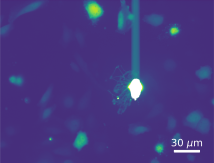
\includegraphics[width=0.35\textwidth]{img/cap_2/saturation.png}
    \caption{\footnotesize{Imagen de ejemplo de un grupo de células donde una de ellas aumentó tanto su intensidad que saturo la cámara y, además, ocurrió un arrastre de electrones a los otros píxeles de la tira afectando la adquisición.}}
    \label{fig:saturacion}
\end{figure}

Habiendo seleccionado los parámetros de adquisición, fue necesario elegir cuantas posiciones adquirir por pocillo. En resultados de análisis previos del grupo, Dr. Klaus Schuermann en Dortmund vio que las células tardaban entre 15 y 30 minutos en clivar su biosensor correspondiente. Por ello, se buscó llevar la resolución temporal de 10 minutos a mínimo 5 minutos y para esto se tuvo en cuenta el tiempo que se tarda en adquirir las imágenes correspondientes a cada polarización y la traslación de la platina motorizada. Cabe destacar que una vez adquirida la imagen, el microscopio tarda alrededor de 90~ms en cambiar de polarizador para adquirir la nueva imagen. Por otro lado, dependiendo la distancia entre las distintas posiciones, la platina tarda entre 1.3 y 2 segundos en trasladarse y entrar en foco (ver \cref{fig:tiempo_adq_un_canal}). El tiempo necesario para que la platina se traslade depende de la distancia entre posiciones, especialmente si esta debe trasladarse dentro de un mismo pocillo o entre pocillos. Dentro de los 5 minutos de resolución temporal, podemos adquirir múltiples posiciones ya que si demoramos como máximo 2 segundos en adquirir las imágenes correspondientes a una posición y trasladarnos a la siguiente, entonces seríamos capaces de adquirir 150 posiciones antes de volver a la primera. Finalmente, cada una de estas posiciones adquiridas suele contener entre 15 y 40 células, por lo que se estima adquirir 2250 a 6000 células por experimento. Una vez seleccionadas la máxima cantidad de posiciones posible de adquirir en menos de 5 minutos, se dejó el microscopio adquiriendo secuencialmente todas las imágenes a lo largo de las 15 horas del experimento. Utilizando una resolución temporal de 5 minutos durante 15 horas se adquieren 180 imágenes de una única polarización y posición, siendo 54000 imágenes en total.

\begin{figure}
    \centering
    \includegraphics[width=0.5\textwidth]{img/cap_2/tiempo_adq_un_canal.pdf}
    \caption{\footnotesize{Esquema de los tiempos característicos de la adquisición secuencial de imágenes en cada polarización. En este caso se usaron 50 ms de tiempo de exposición para adquirir cada imagen, 90 ms entre cada polarización y 2 segundos para que la platina motorizada cambie de posición y entre en foco. El tiempo necesario para cambiar la configuración de polarizadores está incluido en el tiempo necesario para que la platina se traslade de una posición a otra.}}
    \label{fig:tiempo_adq_un_canal}
\end{figure}


%%%%%%%%%%%%%%%%%%%%%%%%%%%%%%%%%%%%
\section{Análisis de Imágenes}


Debido a la elevada cantidad de imágenes típicamente adquiridas durante estos experimentos de microscopía, resulta esencial automatizar el análisis de imágenes. Para ello se generaron y utilizaron diversos algoritmos desarrollados a lo largo del doctorado mediante el lenguaje de programación Python. Algunos de los algoritmos utilizados se encuentran en \href{https://github.com/acorbat/img_manager}{img\textunderscore manager} (ver apéndice \ref{repositorio}) y fueron aplicados a otros trabajos en colaboración como el publicado con \cite{Fernandez-Alvarez2020}. Es crucial considerar la robustez del algoritmo al momento de generarlo ya que podría introducir sesgos en el análisis posterior de la señal obtenida. Veremos en esta sección los distintos pasos del análisis así como errores en algunos de estos pasos se propagan a la señal de anisotropía.

El objetivo del análisis de imágenes es obtener las curvas de anisotropía correspondientes a las células detectadas en cada imagen. Por tratarse de una técnica de alto rendimiento, no es necesario detectar todas las células ya que aunque la eficiencia sea baja, la cantidad detectada será elevada. Podemos separar el análisis en dos partes: una correspondiente a la segmentación y seguimiento de células; y otra a la cuantificación de intensidad de fluorescencia y el cálculo de anisotropía (\cref{fig:analisis_imagenes}).

\begin{figure}
    \centering
    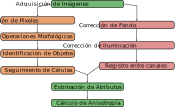
\includegraphics[width=0.7\textwidth]{img/cap_2/analysis_pipeline.png}
    \caption{\footnotesize{Esquema del procedimiento de análisis de imágenes utilizado. Luego de la adquisición de imágenes el proceso se divide en dos que pueden ocurrir en paralelo: segmentación y seguimiento de células; y corrección y cuantificación de intensidad. Una vez segmentadas las células y corregidas las imágenes, se pueden estimar diversos atributos de ellas (tamaño, excentricidad, intensidad de fluorescencia, etc) y luego calcular su anisotropía.}}
    \label{fig:analisis_imagenes}
\end{figure}


%%%%%%%%%%%%%%%%%%%%%%%%%%%%%%%%%%
\subsection{Segmentación y Seguimiento de Células}


En primer lugar, para obtener la información buscada en las imágenes debemos segmentarlas. Este paso consiste en clasificar qué píxeles corresponden a objetos y cuáles a fondo. Existen diversas formas de realizar esta clasificación, desde utilizar un valor umbral para clasificar los píxeles, o primero utilizar kernels específicos para resaltar alguna característica en la imagen, hasta algoritmos de aprendizaje automático donde se utilizan grandes librerías de imágenes ya segmentadas para generar un algoritmo que aprenda a distinguir entre cada clase de píxeles.

Para la clasificación de píxeles se utilizó un algoritmo desarrollado en el laboratorio que se encuentra disponible para descargar de \href{https://github.com/maurosilber/cellment/tree/master/cellment}{Cellment} (ver apéndice \ref{repositorio}). Dicho algoritmo analiza los gradientes de intensidad en la imagen para detectar píxeles que con certeza pertenecen al fondo de la imagen (\cref{fig:clasificacion}B y \ref{fig:clasificacion}C). A partir de estos es capaz de reproducir de forma robusta la distribución de intensidad de los píxeles del fondo. Luego, se puede elegir como umbral para clasificar píxeles algún percentilo de dicha distribución (\cref{fig:clasificacion}A). Para la clasificación se utilizó el percentilo 70 de la distribución de intensidad del fondo (\cref{fig:clasificacion}D).

\begin{figure}[htb]
    \centering
    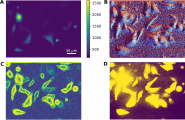
\includegraphics[width=0.9\textwidth]{img/cap_2/clasificacion.pdf}
    \caption{\footnotesize{Análisis de imágenes que lleva a la clasificación de píxeles en fondo y frente. Cabe destacar que aunque las células se vean tenues en la imagen original, es posible distinguirlas en la clasificación. \textbf{A.} Imagen característica de una posición dentro de un pocillo del LabTek de un experimento donde se utilizó staurosporina como estímulo apoptótico. \textbf{B.} Imagen que resulta de estudiar la direccionalidad del gradiente de la imagen cruda suavizada. Este paso es una ayuda visual para interpretar como incrementa la intensidad de fluorescencia desde el borde de la célula al centro debido a su forma. \textbf{C.} Imagen resultante de aplicar el filtro \ening{Silver Mountain Operator} (SMO) a la imagen analizada. Dicho filtro es un paso esencial del análisis utilizado en el algoritmo de Cellment. \textbf{D.} Habiendo hallado la distribución de intensidad del fondo, se utilizó el valor del percentilo 70 para clasificar píxeles en fondo y frente. Notar el patrón en sal y pimienta resultante en la imagen que será corregido en los próximos pasos.}}
    \label{fig:clasificacion}
\end{figure}

Una vez seleccionados los píxeles correspondientes a objetos en la imagen, es necesario eliminar artefactos de la clasificación. Estos se dan principalmente cuando píxeles del fondo toman valores elevados debido a ruido en la medición, formando patrones llamados sal y pimienta, o en los bordes de los objetos ya que las intensidades son bajas y comparables al fondo (\cref{fig:clasificacion}D). Para corregir patrones en sal y pimienta se pueden utilizar métodos que remueven objetos o agujeros pequeños, ya que estos son considerablemente menores que el tamaño típico de nuestro objeto de interés. Por otro lado, hay operaciones morfológicas que consisten en cambiar la clase de un píxel según si en su vecindad hay un píxel correspondiente a fondo (erosión) o frente (dilación). Estas operaciones se pueden aplicar sucesivamente para suavizar bordes, conectar estructuras e incluso eliminar el patrón en sal y pimienta. Notar que el orden en que se aplica la erosión y dilación no es indistinto y se denominan apertura, erosión seguido de dilación, y clausura, el orden inverso. Particularmente, se aplicó una clausura definiéndose como vecindad un disco de radio 10 píxeles (\cref{fig:seguimiento}A y B).

Luego de separar los píxeles correspondientes al frente y fondo, debemos separar el frente en cada uno de los objetos que lo componen, en este caso, células. En raras ocasiones, las células se encuentran suficientemente alejadas unas de otras como para ser identificadas como objetos separados, mientras que en la mayoría de los casos debemos separarlas por otros métodos. Si tenemos en cuenta que, dada la morfología celular, el centro de las células es más intenso que los bordes, se pueden utilizar algoritmos como \ening{watershed} para separarlas. Este algoritmo toma como entrada semillas que marcan las posiciones en donde hay células y luego utiliza la topografía formada por la intensidad de la imagen para separarlas entre sí. Como punto de partida, se utilizaron los máximos locales de intensidad (\cref{fig:seguimiento}C y D).

\begin{figure}[htb]
    \centering
    \includegraphics[width=0.9\textwidth]{img/cap_2/seguimiento.pdf}
    \caption{\footnotesize{Análisis de imágenes que permitió reconocer objetos (células) y seguirlos a lo largo de la serie temporal. \textbf{A.} Imagen de ejemplo analizada con el contorno que resulta de aplicar operaciones morfológicas sobre la imagen de clasificación de píxeles. \textbf{B.} A la clasificación presentada en la \cref{fig:clasificacion}D se le aplico una operación morfológica de clausura definiendo como vecindad un disco de radio 10 píxeles. \textbf{C.} Imagen de ejemplo analizada con el contorno de las células reconocidas por el algoritmo de seguimiento. \textbf{D.} Imagen que resulta de separar en las distintas células, luego del análisis de seguimiento, los objetos hallados en el frente de la imagen presentada en \textbf{B}.}}
    \label{fig:seguimiento}
\end{figure}

Habiendo identificado a las células como objetos distintos en las sucesivas imágenes, y sabiendo que estas pueden trasladarse a lo largo del experimento, será necesario seguirlas a lo largo de la serie temporal. Dado que el traslado de las células en estudio es chico en relación a su área en esta escala de tiempo, esto se logró comparando el área superpuesta entre objetos en imágenes subsiguientes. Puede darse la situación en que la cantidad de objetos detectados sea distinta entre imágenes. En algunos casos, esto puede deberse a que hubieron defectos en segmentación y separación de células contiguas. Esta información es utilizada para separar células que no fueron adecuadamente separadas en los pasos previos. En el caso de experimentos de apoptosis, esto es fácil de identificar cuando células contiguas se desprenden del vidrio en momentos distintos ya que cambian su forma y se separan una de otra, siendo fácilmente separables. Esta información puede utilizarse para separar las células en imágenes previas (\cref{fig:seguimiento}D y \cref{fig:track_many}).

\begin{figure}
    \centering
    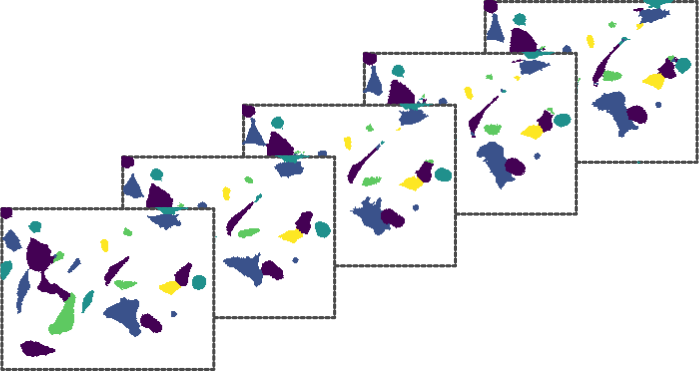
\includegraphics[width=0.7\textwidth]{img/cap_2/tracking_many.pdf}
    \caption{\footnotesize{Secuencia de imágenes de ejemplo para mostrar el algoritmo de seguimiento de células. Se muestran una de cada 5 imágenes correspondientes a la imagen de muestra utilizada previamente. Cada color corresponde a una célula distinta que fue seguida a lo largo de la secuencia.}}
    \label{fig:track_many}
\end{figure}


%%%%%%%%%%%%%%%%%%%%%%%%%%%%%%%%%
\subsection{Estimación de Anisotropía}
\label{sec:matmet:CalculoAnisotropia}


Una vez segmentadas las células y habiendo completado el seguimiento de ellas a lo largo de la serie temporal, debemos estimar su intensidad de fluorescencia en cada imagen. Para ello será necesario aplicar primero diversas correcciones a las imágenes. Por ejemplo, corregir inhomogeneidades en la iluminación, el fondo y posibles desplazamientos entre los canales adquiridos (\cref{fig:analisis_imagenes}). Además, por tratarse de anisotropía de fluorescencia, será necesario corregir el factor G, es decir, las diferencias en ganancia y depolarizaciones que pueden haber en la adquisición de las distintas polarizaciones.

El primer paso fue corregir el fondo de las imágenes. Para ello, se aprovechó que conocíamos con bastante certeza los píxeles correspondientes al fondo y sus posiciones. Esto ayudó a generar una imagen que surgía de interpolar una superficie suave que pase por los píxeles oscuros detectados (\cref{fig:correcciones}A). A nuestra imagen de interés le debemos restar la superficie interpolada. Luego discutiremos los efectos en el cálculo de anisotropía que surgen de errores en la estimación de fondo.

\begin{figure}[htb]
    \centering
    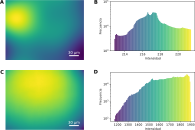
\includegraphics[width=0.9\textwidth]{img/cap_2/correcciones.pdf}
    \caption{\footnotesize{Imágenes de fondo e iluminación utilizadas para corregir las imágenes obtenidas. \textbf{A.} Imagen del fondo estimado para el ejemplo analizado. Las inhomogeneidades corresponden al brillo  fuera de foco de las células. Cabe destacar que las diferencias de intensidades son del orden de la decena. \textbf{B.} Histograma de intensidades correspondientes al fondo estimado. Notar que los valores se encuentran alrededor de 200 que corresponden al fondo de la cámara. \textbf{C.} Imagen correspondiente a la normalización utilizada. Esta imagen surge de calcular la mediana píxel a píxel de varias imágenes de fluoresceína diluida. \textbf{D.} Histograma de intensidades correspondientes a la imagen de normalización obtenida. Notar que la población de píxeles poco iluminados es considerablemente menor que los más iluminados.}}
    \label{fig:correcciones}
\end{figure}

A continuación, se corrigieron las inhomogeneidades en la iluminación. Para ello, se adquirieron diez imágenes de fluoresceína diluida en cada polarización utilizando el mismo armado experimental. Se generó una única imagen que consistió en la mediana para cada píxel de las distintas imágenes (\cref{fig:correcciones}C). Ésta imagen fue utilizada para realizar una división píxel a píxel de todas las imágenes adquiridas. Como se mencionó previamente, la fluoresceína diluida tiene un valor nulo de anisotropía y, por lo tanto, también sirve como corrección de factor G. En la figura \ref{fig:correcteds} puede apreciarse el resultado de aplicar las sucesivas correcciones.

\begin{figure}[htb]
    \centering
    \includegraphics[width=0.9\textwidth]{img/cap_2/correcteds.pdf}
    \caption{\footnotesize{Imágenes original y corregida con sus respectivos histogramas de intensidad. \textbf{A.} Imagen de ejemplo analizada. \textbf{B.} Histograma de intensidades obtenidos de la imagen que será analizada. Notar que la cámara de 12 bits tiene un rango dinámico de hasta 4096 y se decidió no usar la totalidad de éste para que no saturen las imágenes subsiguientes. \textbf{C.} Imagen corregida que resulta de restarle el fondo y normalizar a la imagen original. \textbf{D.} Histograma correspondiente a la imagen corregida. Se puede apreciar que los valores de intensidad corresponden a las distintas células presentes en la imagen.}}
    \label{fig:correcteds}
\end{figure}

Corregir adecuadamente la inhomogeneidad en la iluminación, el fondo y factor G es esencial para una correcta estimación de la intensidad de fluorescencia. Por medio de un código interactivo (\href{https://github.com/acorbat/anisotropy_errors/tree/master/anisotropy_errors}{anisotropy\textunderscore errors}, ver apéndice \ref{repositorio}) se analizó la propagación de cometer errores en la estimación de intensidad paralela o perpendicular. Es trivial notar que un error sistemático trasladará y reescalará la curva de anisotropía. Es decir, la forma se mantendrá pero la anisotropía del dímero y monómero serán distintos a lo esperado (ver \cref{fig:error_bkg}). Por otro lado, dependiendo de la magnitud de este error, podría ocurrir que la anisotropía del monómero sea menor que la del dímero, produciendo una inversión de la curva. Por último, debemos destacar que si el error varía a lo largo del tiempo, esto puede cambiar la forma de la curva y llevar a mayor confusión y dificultad a la hora de corregirlo.

\begin{figure}[htb]
    \centering
    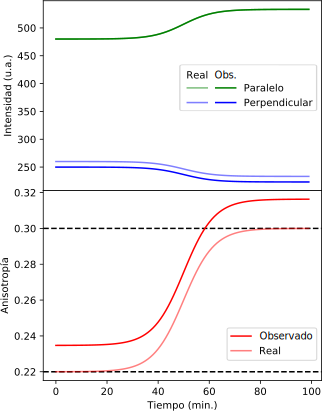
\includegraphics[width=0.5\textwidth]{img/cap_2/error_bkg.pdf}
    \caption{\footnotesize{Simulación de curvas de intensidad paralela y perpendicular donde se cometió un error de solo 10 unidades en la estimación del fondo de la imagen perpendicular, que corresponde a menos del 5\%. Dicho error se traduce en un corrimiento de la curva de anisotropía de 0.02 que representa alrededor de un 10\%.}}
    \label{fig:error_bkg}
\end{figure}

Luego, debemos corregir posibles desplazamientos entre las imágenes de los distintos canales. Aunque este efecto suele ser pequeño cuando se utilizan distintos filtros de emisión, es mucho más pronunciado al cambiar de polarizador. Esto se debe principalmente a que los polarizadores utilizados son gruesos (7~mm) ya que el grosor se asocia a su calidad. Si consideramos al polarizador como dos cambios de medio paralelos, podemos realizar un análisis de trayectoria de rayos para entender que si el haz incide en algún ángulo no perpendicular, el polarizador trasladará el haz una distancia que dependerá de su grosor, sin afectar su direccionalidad.

\begin{figure}[b!]
    \centering
    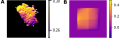
\includegraphics[width=0.6\textwidth]{img/cap_2/shifts.png}
    \caption{\footnotesize{Imágenes de anisotropía calculadas a partir de imágenes de intensidad que están desplazadas una respecto de la otra. \textbf{A.} Imagen correspondiente a una célula observada experimentalmente. Puede apreciarse que en la región superior los valores de anisotropía calculados son más altos que en la sección inferior. \textbf{B.} Imagen de anisotropía generada a partir de una célula con forma piramidal simulada utilizando anisotropy\textunderscore errors.}}
    \label{fig:shifts}
\end{figure}

El patrón generado en la imagen de anisotropía por este tipo de errores de registro entre canales es fácilmente identificable y se aprecia como sombras topográficas (ver  \cref{fig:shifts}). Consideremos un objeto con un gradiente de intensidad, como suele suceder en el citoplasma de algunas células. Al estar desplazadas las imágenes, siempre se restarán valores desfasados del gradiente de intensidad. Esto resultará en que los valores de anisotropía estarán corridos hacía valores mayores o menores dependiendo de la dirección del gradiente respecto a la dirección del desplazamiento, generando una imagen de aspecto sombreada. Esto se exacerba aún más en los píxeles del borde del objeto, donde alguna de las intensidades será casi nula por corresponder al fondo, resultando en valores extremos de anisotropía.

Mediante simulaciones de imágenes de intensidades paralela y perpendicular (ver \href{https://github.com/acorbat/anisotropy_errors/tree/master/anisotropy_errors}{anisotropy\textunderscore errors} y \cref{fig:shifts}) se estudió la forma más robusta de estimar la anisotropía de cada objeto. A grandes rasgos y considerando que el cálculo de anisotropía es no lineal, es posible calcular la imagen de anisotropía y promediar los valores obtenidos o promediar en las imágenes de intensidades y calcular la anisotropía. Cabe destacar que si quisiéramos calcular la imagen de anisotropía, debemos ser capaces de corregir ambas imágenes de intensidad lo mejor posible. En el caso de corregir desplazamientos entre imágenes, puede ser necesario hacer una traslación subpíxel, es decir, una distancia menor al tamaño de un píxel. Para lograr esto último sería necesario interpolar entre los píxeles adquiridos de la imagen, proceso que suele incrementar el ruido.

\begin{figure}[t!]
    \centering
    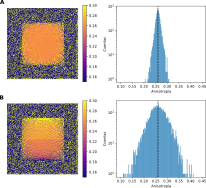
\includegraphics[width=0.75\textwidth]{img/cap_2/anisotropy_variances.pdf}
    \caption{\footnotesize{Si simularon células de forma piramidal con los biosensores dentro tomados de distribuciones al azar. El ensamble de biosensores se simuló de tal forma que su anisotropía sea 0.26. A la izquierda se ven las imágenes de anisotropía de las célula adquiridas y corregidas perfectamente (\textbf{A}) o con un shift de un píxel en el eje vertical (\textbf{B}). A la derecha se grafican los histogramas de anisotropía de los píxeles de la célula, ignorando el borde de esta ya que es muy ruidoso debido a la baja intensidad. Se puede apreciar que este leve error en la corrección del corrimiento no solo generó una imagen fácilmente distinguible, sino que también esto hace que la varianza aumente considerablemente. Notar que con un pequeño corrimiento de un píxel la media no varía de forma apreciable, pero este efecto será mayor para corrimientos más grandes. Por otro lado, si el corrimiento es menor a un píxel, es necesario interpolar los valores entre píxeles y esto puede exacerbar el ruido de cada píxel.}}
    \label{fig:anisotropy_variance}
\end{figure}

Se comprobó que errores de registro aumentan la variabilidad de la anisotropía de la célula adquirida, por lo que se consideró barrer en los valores de desplazamiento y minimizar dicha varianza (ver \cref{fig:anisotropy_variance}). Más allá del costo computacional elevado que tenía este procedimiento, se verificó que estimar la suma de intensidades y luego calcular la anisotropía no solo era más eficiente, sino también más robusto. Esto se debía principalmente a que al promediar las intensidades cualquier error de registro remanente era compensado por otras regiones del objeto. Además, al erosionar las células era fácil descartar los píxeles del borde correspondientes a los menos intensos. Por último, calcular la sumatoria de intensidades, equivalente al promedio ya que la anisotropía se normaliza, antes del cálculo de anisotropía es estadísticamente favorable ya que el ruido de cada píxel no se propaga a través del cálculo no lineal.


%%%%%%%%%%%%%%%%%%%%%%%%%%%%%%
\section{Modelado de la Cinética Enzimática}
\label{sec:CineticaEnzimatica}


Las enzimas son catalizadores, en general proteínas, que colaboran en la conversión de sustratos en producto, manteniéndose inalteradas una vez terminada la reacción. Entre sus características más importantes encontramos su elevado poder catalítico, su especificidad y la posibilidad de regularlas. Estas son especialmente eficientes para acelerar reacciones biológicas, aumentando hasta 10 millones de veces la velocidad de reacción. Típicamente se encuentran reguladas por una complicada red de lazos de retroalimentación, tanto positivos como negativos, permitiendo un control preciso sobre la tasa de reacción \citep{Keener2009}.

Las caspasas en estudio son enzimas, en particular, proteasas. Realicemos el experimento mental de modelar un biosensor de caspasas, o cualquier proteasa, como el introducido en el trabajo de \cite{Stegemann2015}. Esto nos servirá para comprender su funcionamiento y entender las razones detrás de cada paso del análisis de datos. Estos biosensores son sintetizados por la célula en su estado dimérico y luego procesados por la caspasa en cuestión una vez activa. Esto es análogo a un sustrato, biosensor dimérico, que es procesado por una enzima, caspasa, para dar lugar de forma irreversible a un producto, biosensor monomérico.

Un modelo para describir esta cinética fue propuesto por Michaelis y Menten. En el esquema de la reacción, la enzima ($E$) convierte al sustrato ($S$) en producto ($P$) en un proceso de dos pasos. En el primer paso, se unen la enzima y el sustrato formando un complejo enzima-sustrato ($C$); para luego dar lugar a la formación del producto y la liberación de la enzima. Esta reacción puede representarse como

\begin{center}
\ce{S + E <=>[$k_+$][$k_-$] C ->[$k_c$] P + E.}
\end{center}

\noindent Aunque en general el producto puede volver a unirse a la enzima, y estas aceleran las reacciones en ambos sentidos, en nuestro caso particular, el biosensor una vez clivado no vuelve a su estado dimérico.

El siguiente paso consiste en aplicar ley de acción de masas para describir el cambio en la concentración de cada una de las especies a partir las constantes cinéticas de cada reacción. Comencemos por considerar una reacción simple en la que el sustrato $S$ y la enzima $E$ colisionan para formar $C$, es decir,

\begin{center}
\ce{S + E ->[$k_+$] C,}
\end{center}

\noindent donde $k_+$ se denomina la constante de reacción. Ésta surge de considerar que las colisiones de las moléculas en el sistema en equilibrio térmico se dan de forma completamente aleatoria. Esta constante depende a su vez de la relación entre los tamaños de las especies involucradas, su geometría y otros parámetros que pueden reducirse a la probabilidad de encuentro y reacción exitosa \citep{Gillespie1977}.

Asumiendo que la concentración de las especies en estudio pueden ser descriptas mediante funciones continuas, y que cada una de sus reacciones químicas pueden representarse como procesos continuos, es posible construir una serie de ecuaciones diferenciales acopladas que describan la dinámica. En este caso particular, la variación de la concentración del complejo ($C$) descripta por \cite{Gillespie1977} es

\begin{equation}
    \frac{dC}{dt} = k[S][E],
\end{equation}

\noindent donde $[S]$ y $[E]$ se refieren a las concentraciones de sustrato y enzima respectivamente. Al igual que la ley de Ohm o la ley de Newton para enfriamiento, esta tiene cierto rango de validez. En primer lugar, si se trabaja a concentraciones altas, duplicar la concentración no implica que necesariamente se duplique la tasa de formación de producto. En el otro extremo, si se utilizan concentraciones muy bajas, puede que representar la concentración como una variable continua no sea la mejor opción \citep{Keener2009}.

Analicemos las ecuaciones diferenciales que surgen al aplicar ley de acción de masas al sistema completo

\begin{align}
    \frac{ds}{dt} =& k_- c - k_+ se \label{eq:cin_sens}\\
    \frac{de}{dt} =& (k_- + k_c) c - k_+ se\\
    \frac{dc}{dt} =& k_+ se - (k_- + k_c) c\\
    \frac{dp}{dt} =& k_c c, \label{eq:cin_prod}\\
\end{align}

\noindent donde se uso que $[E]=e$, $[S]=s$, $[C]=c$ y $[P]=p$. Podemos apreciar que $\frac{de}{dt} + \frac{dc}{dt} = 0$, que corresponde a la existencia de una cantidad conservada, en este caso la enzima. Esto se condice con lo explicado previamente ya que la enzima acelera la reacción, pero se mantiene inalterada una vez culminada. De aquí que $e+c=e_0$ donde $e_0$ es la cantidad de enzima disponible. Por otro lado, también se aprecia que $\frac{ds}{dt} + \frac{dc}{dt} + \frac{dp}{dt} = 0$, que, dado que no hay síntesis de sustrato ni degradación de producto incluidas hasta ahora, se conserva la cantidad de sustrato más producto en todos sus estados.

\begin{figure}[b!]
    \centering
    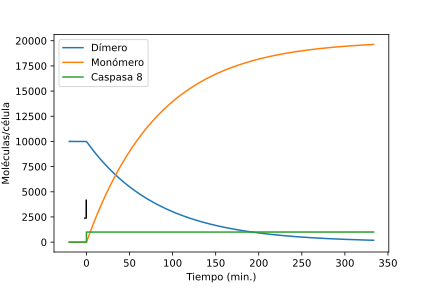
\includegraphics[width=0.6\textwidth]{img/cap_2/ejemplo_enzima.pdf}
    \caption{\footnotesize{Simulación a modo de ejemplo donde la caspasa 8 procede a clivar su biosensor correspondiente. Se comenzó con una concentración inicial de 10000 moléculas de biosensor y a tiempo cero se agregan 1000 moléculas por célula de la caspasa 8. Notar que a tiempos largos, la cantidad de moléculas por celula de biosensor clivado es el doble que la de biosensors dimérico al principio debido a que pasó a estado monomérico. Las constantes cinéticas seleccionadas fueron similares a las encontradas en modelos publicados.}}
    \label{fig:ejemplo_enzima}
\end{figure}

A modo de ejemplo, creemos un modelo en PySB \citep{Lopez2013} en donde vamos a definir las reacciones correspondientes al clivaje de un biosensor dimérico por parte de la caspasa 8. Utilizaremos como constantes cinéticas valores típicos hallados en la bibliografía, a saber, $k_+ = 10^{-7}$, $k_- = 10^{-3}$ y $k_c = 1$. En cuanto a concentraciones iniciales, utilizaremos 1000 moléculas por célula de caspasa 8 y 10000 moléculas de biosensor en estado dimérico. Podemos apreciar que una vez clivado todo el sensor, tendremos 20000 moléculas por célula de biosensor en estado monomérico (ver \cref{fig:ejemplo_enzima}).

Notemos que el biosensor utilizado es irreversible, por lo que no mide directamente la actividad de la caspasa, sino su integral. Utilizando la ecuación \ref{eq:cin_prod} que relaciona la velocidad de formación de producto, o sensor clivado en este caso, con la concentración de complejo, podemos interpretarla como la cantidad de caspasa que se encuentra clivando sensor en cada instante, es decir, ofrece una lectura sobre la actividad caspasa.


%%%%%%%%%%%%%%%%%%%%%%%
\section{Estimación del Observable Biológico}
\label{sec:Observable}


A continuación, debemos traducir los valores de anisotropía hallados para cada célula en una propiedad que refiera a la caspasa, o enzima, en estudio. Supongamos entonces una población de biosensores con una concentración ($[C]$) que se encuentra una parte en estado dimérico ($[D]$) y otra en estado monomérico ($[M]$). Si tenemos en cuenta que los distintos fluoróforos poseen propiedades fotofísicas diferentes, como sus espectros de absorción y emisión, su rendimiento cuántico, el estado madurativo de los fluoróforos que lo componen, entre otras, entonces sus brillos por molécula detectados serán diferentes. Esto quiere decir que las intensidades de cada subpoblación de fluoróforos será

\begin{align}
    I_M &= (b_{M_1} + b_{M_2}) M\\
    I_D &= (b_{M_1} + b_{M_2} + \delta b) D,
\end{align}

\noindent donde se asumió que la concentración de cada tipo de fluoróforo en estado monomérico es igual ya que los biosensores se sintetizan como dímeros y luego son clivados. Los brillos de cada fluoróforo son $b_{M_1}$ y $b_{M_2}$, mientras que en el caso del dímero, a estos brillos se les suma $\delta b$ ya que debido a la transferencia de energía entre ellos, el brillo detectado dependerá de qué fluoróforo emita con mayor intensidad.

\begin{figure}[htb]
    \centering
    \includegraphics[width=0.6\textwidth]{img/cap_2/anisotropy_sensors.png}
    \caption{\footnotesize{Los biosensores son sintetizados en forma dimérica por las células y en este estado tienen una anisotropía de polarización baja debido a FRET entre fluoróforos. Una vez clivados, estos biosensores no pueden volver al estado previo y sirven como reporteros de la actividad integral de las caspasas. Al clivarse todo el ensamble de biosensores, se interrumpe el FRET entre fluoróforos y se alcanza un nivel de anisotropía de polarización más elevado. Adaptado de \cite{Corbat2018}.}}
    \label{fig:anisotropia_biosensor}
\end{figure}

Considerando que la anisotropía del conjunto de biosensores nos refiere al estado de dicha población a través del promedio pesado de sus intensidades (ver \cref{fig:anisotropia_biosensor}), es decir, 

\begin{equation}
r = \frac{\sum_i I_i r_i}{\sum_i I_i}, \label{eq:anisotropiaInt}
\end{equation}

\noindent donde $I_i$ corresponde a la intensidad del biosensor en un estado y $r_i$ su anisotropía. Suponiendo además que la concentración de biosensores se mantiene constante, 

\begin{equation}
    [C] = [M] + 2[D],
    \label{eq:C_cte}
\end{equation}

\noindent podemos despejar $m = [M]/[C]$, la fracción de biosensores en estado monomérico en función de las anisotropías

\begin{equation}
	m = \frac{b (r - r_D)}{r_M - r + b (r - r_D)},
	\label{eq:m_from_r}
\end{equation}

\noindent donde $r_D$ y $r_M$ corresponden a las anisotropías del dímero y monómero respectivamente; y donde $b=B_D/B_M = (b_{M_1} + b_{M_2} + \delta b) / (b_{M_1} + b_{M_2})$ es la relación entre brillos. De esta forma, podemos traducir anisotropía en la fracción de biosensor en estado monomérico y viceversa, pasando por valores esperados de intensidad de fluorescencia en cada polarización (ver \cref{fig:mono_to_ani}).

\begin{figure}[htb]
    \centering
    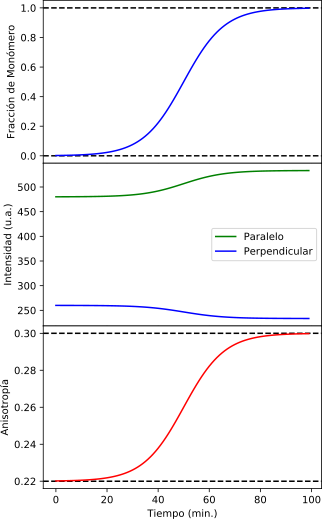
\includegraphics[width=0.5\textwidth]{img/cap_2/mono_to_ani.pdf}
    \caption{\footnotesize{Se generó una curva ejemplo de fracción de biosensor en estado monomérico en función del tiempo y se estimaron sus intensidades en los canales paralelo y perpendicular a la excitación. A continuación, es posible traducir la curva de fracción de monómero, así como las de intensidades, en la curva correspondiente de anisotropía en función del tiempo. Para todo ello es necesario conocer los valores de anisotropía del dímero y monómero, así como $\Delta b$.}}
    \label{fig:mono_to_ani}
\end{figure}

Teniendo en cuenta que el biosensor es irreversible, este solo puede medir la actividad integral de la enzima bajo estudio (\cref{fig:anisotropia_biosensor}). Por esta razón, uno debe calcular su derivada para obtener la actividad enzimática instante a instante (como se menciona al final de la sección \ref{sec:CineticaEnzimatica}), es decir,

\begin{equation}
	\dot{m} = \frac{1 + \Delta b}{r_M - r_D} \frac{\dot{r}}{\left[1 + \Delta b \frac{r - r_D}{r_M - r_D}\right]^2}.
	\label{eq:m_der}
\end{equation}

\noindent donde $1 + \Delta b = (b_{M_1} + b_{M_2} + \delta b) / (b_{M_1} + b_{M_2})$ es la relación entre los brillos del dímero sobre los del monómero. Cabe destacar que dichas propiedades no solo dependen del fluoróforo utilizado sino también del sistema de detección utilizado. Notar que si el brillo detectado de ambos monómeros es igual al del dímero, $\Delta b = 0$, entonces la derivada de la fracción de monómero es proporcional a la derivada de anisotropía (ver \cref{fig:sweep_b}). 

Consideremos el error que se genera al no utilizar el parámetro $\Delta b$. Analicemos brevemente la ecuación \ref{eq:m_der} que nos dice que el máximo de actividad, dado por el máximo de la derivada del cambio de fracción de monómero depende de la derivada de la curva de anisotropía, dividida por $\left[1 + \Delta b \frac{r - r_D}{r_M - r_D}\right]^2$. Donde el segundo término dentro de la potencia es la curva de anisotropía normalizada por sus valores extremos, anisotropía del dímero y monómero, multiplicada por $\Delta b$. Eso quiere decir que el máximo de actividad estará cerca de donde la curva de anisotropía cambie de valor y que éste se verá afectado por el denominador cuando $\Delta b$ sea distinto de 0. Teniendo esto en cuenta, es de esperarse que utilizar un valor erróneo nos dará un error sistemático de unos pocos minutos ya que el transcurso de tiempo en el que cambia la curva es de ese orden (ver \cref{fig:sweep_b}).

\begin{figure}[htb]
    \centering
    \includegraphics[width=0.9\textwidth]{img/cap_2/sweep_b_mono_ders.pdf}
    \caption{\footnotesize{Sabiendo como traducir la curva de fracción de monómero en anisotropía y viceversa, es posible también calcular la actividad enzimática instante a instante. \textbf{A.} Se simuló una curva de fracción de biosensor en estado monomérico y se muestra la equivalencia entre su derivada y la curva de actividad instante a instante. \textbf{B.} Se simularon curvas de anisotropía a partir de la misma curva de fracción de monómero pero variando el parámetro $\Delta$b entre -0.3 y 0.3, es decir, se varió $b$ entre 0.7 y 1.3. Se puede apreciar como las curvas de anisotropía y sus derivadas se corren dependiendo del valor de b, sin embargo, la curva calculada de actividad es siempre la misma.}}
    \label{fig:sweep_b}
\end{figure}

Conociendo el formalismo teórico detrás del funcionamiento del biosensor utilizado, debemos ser capaces de calcular la actividad enzimática a partir de las curvas de anisotropía obtenidas luego del análisis de imágenes. Para ello, necesitaremos estimar la derivada de las curvas de anisotropía, así como los valores de anisotropía del monómero y dímero. Debido al ruido de alta frecuencia y la necesidad de calcular divisiones donde el denominador suele ser considerablemente menor que el numerador, derivar es una operación computacionalmente mal definida. Por estas razones, se evaluaron distintos métodos para calcular la derivada de las curvas de anisotropía obtenidas a partir del análisis de imágenes. En primer lugar se consideró realizar ajustes con curvas sigmoideas y luego derivarlas, pero no todas las actividades presentaban un perfil sigmoideo por lo que se decidió no proseguir. En segundo lugar, se consideró utilizar diferencias finitas. Aunque dicho algoritmo sopesa adecuadamente los puntos más cercanos para hallar la derivada, tiene problemas cuando hay puntos faltantes. Finalmente, se implementó un filtro savitzky-golay. Dicho filtro hace un ajuste polinomial de bajo grado en una ventana móvil de un número impar de puntos. El valor del polinomio del punto intermedio puede utilizarse para reemplazar el valor de la curva experimental, sirviendo de suavizado, o puede utilizarse para estimar la derivada en dicho punto. La principal desventaja de éste es que al suavizar la curva, el máximo de la derivada puede disminuir aunque no se espera ver un corrimiento pronunciado. Luego se procedió a interpolar con splines de grado 3 para obtener los valores de actividad entre cada punto experimental y tomar el tiempo de máxima actividad (ver \cref{fig:savgol_test}).

\begin{figure}[htb]
    \centering
    \includegraphics[width=0.4\textwidth]{img/cap_2/savgol_test.pdf}
    \caption{\footnotesize{A partir de una curva de anisotropía simulada se generaron 1000 realizaciones de la misma con ruido experimental añadido y tomando valores cada 5 minutos (superior). Se estimaron las derivadas con el filtro Savitzky-Golay y se procedió a interpolar con splines de grado 3 para obtener los valores de actividad entre cada punto experimental (medio). Finalmente, se tomaron los valores de máximo de actividad devueltos por cada realización y se confeccionó un histograma (inferior). El valor medio recuperado se corresponde con el máximo de actividad estimado de la curva real y el desvío estándar obtenido fue de 1.9 minutos.}}
    \label{fig:savgol_test}
\end{figure}

Finalicemos con un breve análisis de como calcular el denominador de la derivada de la fracción de monómero. Para ello es necesario estimar propiedades fotofísicas de cada biosensor. Por un lado, el valor de $\Delta b$ puede calibrarse a partir de experimentos. Por otro lado, los valores de anisotropía de dímero y monómero se estimaron para cada curva en particular ya que, como se discutió previamente, son susceptibles a variar debido a la propagación de errores. Una estimación típica de la curva de actividad a partir de la anisotropía se halla en la \cref{fig:derivacion_tipica}.

\begin{figure}[htb]
    \centering
    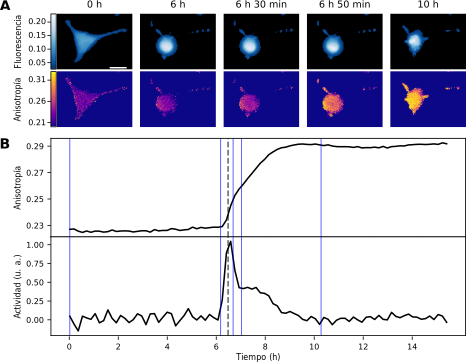
\includegraphics[width=0.9\textwidth]{img/cap_2/typical_derivation.pdf}
    \caption{\footnotesize{Análisis típico de una serie temporal de anisotropía. Adaptado de \cite{Corbat2018}. \textbf{A.} Imágenes de intensidad de fluorescencia y anisotropía correspondientes a una célula observada experimentalmente. Se puede apreciar como cambia la anisotropía a medida que la célula entra en apoptosis mientras que no varía fuertemente en intensidad. \textbf{B.} En el gráfico superior se muestra la anisotropía en función del tiempo de la célula analizada. Las líneas azules verticales corresponden a los tiempos de las imágenes mostradas en \textbf{A}. En el gráfico inferior se muestra la curva de actividad obtenida al analizar la curva de anisotropía.}}
    \label{fig:derivacion_tipica}
\end{figure}

Una vez generadas las curvas de actividad enzimática en función del tiempo, debemos definir un observable que sirva de referencia al momento en que se activaron las enzimas en estudio. Es común hallar en la bibliografía que se utilice el tiempo en el que algún porcentaje de biosensor es clivado (10\%, 50\% ó 90\%). Estos valores pueden determinarse mejor cuando la pendiente es elevada en los momentos alrededor del porcentaje de interés. 

Tratándose de perfiles de actividad enzimática, estos suelen seguir una forma sigmoidea o hiperbólica según las constantes cinéticas presentadas en la sección \ref{sec:CineticaEnzimatica}. Cuando el perfil de la curva tiene una forma sigmoidea, es fácil determinar el momento en que la mitad del biosensor es clivado, mientras que, si la curva tiene algo de ruido, se dificulta determinar el momento en que 10\% o 90\% del biosensor es clivado. Por otro lado, en los casos donde el perfil de clivaje es hiperbólico, esta mejor determinado el momento en que 10\% del sensor es clivado, en cambio el 90\% de clivaje tiene mucho error en su determinación.

Considerando que nuestro objetivo es obtener un tiempo que sirva de referencia de la activación de la enzima y que poseemos información de la actividad enzimática para todo tiempo, se evaluó utilizar el momento en el que se alcanza el máximo de actividad (\cref{fig:curvas_tipicas}). Determinarlo depende principalmente de la resolución temporal ya que sabemos con certeza que debe ubicarse entre los valores más elevados hallados. De esto se deriva la principal ventaja que es que dicha determinación puede ser utilizada sin importar el perfil de clivaje del biosensor. Además, dicho momento puede ser comparado fácilmente con simulaciones de la actividad enzimática. En búsqueda de mayor resolución temporal se utilizó una interpolación de bajo grado para hallarlo.

\begin{figure}[t!]
    \centering
    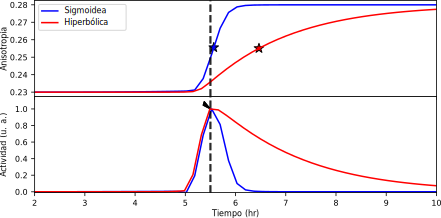
\includegraphics[width=0.9\textwidth]{img/cap_2/sim_analysis.pdf}
    \caption{\footnotesize{Se simularon dos perfiles de anisotropía típicos que se pueden hallar en experimentos con distintas enzimas: sigmoideo (azul) e hiperbólico (rojo). Las estrellas marcan el instante en el que se cliva 50\% del sensor y se puede apreciar que tiene distintas pendientes según la curva y ocurren en distintos momentos. La línea a trazos vertical marca el momento en el que se alcanza la máxima actividad de la enzima. Este momento es fácilmente determinado experimentalmente y puede ser relacionado fácilmente con las simulaciones. Adaptado de \cite{Corbat2018}.}}
    \label{fig:curvas_tipicas}
\end{figure}

En resumen, el flujo de análisis de datos comenzó con la adquisición del orden de cientos de imágenes por canal, entre las que se hallaron del orden de miles de células. Luego de procesar las imágenes, obtener las curvas de actividad para cada célula, se debió filtrar las curvas que correspondían a eventos apoptóticos y estimar el tiempo de máxima actividad de la caspasa en estudio. Cabe destacar que este flujo se puede caracterizar como de alto rendimiento al analizar miles de células, así como de reducción de datos ya que se obtiene un valor característico por cada curva.

%%%%%%%%%  Biosensores
\chapter{Construcción y Caracterización de los Biosensores}
\label{cap:Biosensores}

Teniendo en cuenta un esquema simplificado de la red apoptótica, podemos apreciar que como mínimo nos interesaría poder visualizar la actividad de tres nodos, uno en cada módulo. Dado que cada uno se caracteriza por tener al menos una caspasa, podemos utilizar tres sensores análogos que sean sensibles a distintas proteasas. Además, para poder ubicar los tres sensores en el espectro accesible por las cámaras del microscopio, necesitaremos que los fluoróforos estén basados en homoFRET. Si considerásemos sensores basados en heteroFRET, cada sensor necesita un rango del espectro para el dador y el aceptor separados, imposibilitando el uso de más de dos biosensores simultáneamente. En este capítulo detallaré cómo se seleccionaron los pares de fluoróforos para construir los biosensores \citep{Corbat2018}. Finalmente, dado que los biosensores añadidos de forma exógena en las células introducen perturbaciones en la red estudiada, se caracterizó y redujo la variabilidad introducida en el sistema \citep{Habif2021}.

\section{Selección de Especies de Fluoróforos}

A partir de datos preliminares del grupo, se utilizaron tres pares de fluoróforos cuyos espectros prácticamente no se superponen entre si. Dicho estudio comenzó con un análisis de la distancia de Förster ($R_0$) característica de distintos pares de fluoróforos. Se generaron los constructos en tandem de las combinaciones con mayor $R_0$ y se evaluó experimentalmente la anisotropía del dímero y monómero. Cabe destacar que en los extremos del espectro, rango de los azules y rojos, es difícil encontrar un par de fluoróforos idénticos con elevado rango dinámico de valores de anisotropía. Por esta razón, se consideraron fluoróforos distintos con espectro de excitación y emisión similares. Esto trae aparejada la ventaja que los valores de anisotropía están dados, no solo por los cambios de polarización, sino también por los cambios en la detección. Es decir, la anisotropía dependerá también de la combinación de filtros y lentes utilizados (ver \cref{fig:fluopairs}).

\begin{figure}[t!]
    \centering
    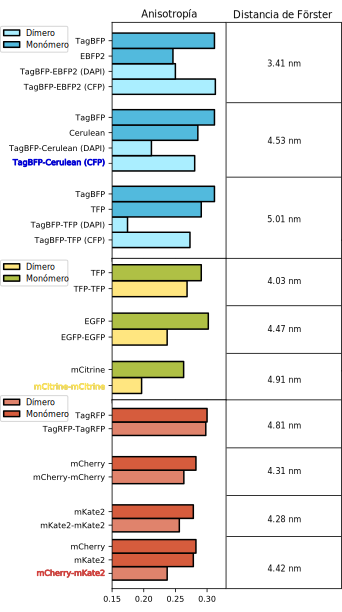
\includegraphics[width=0.6\textwidth]{img/cap_3/fluorophore_pairs.pdf}
    \caption{\footnotesize{Se muestran las anisotropías medidas experimentalmente de los distintos pares de fluoróforos evaluados, así como las distancias de Förster calculadas para cada par. Se debe destacar que cuando fue posible, se midió la anisotropía utilizando un conjunto de filtros distintos ya que éstos afectarán la anisotropía detectada. Notar que en los extremos del rango visible se utilizaron fluoróforos distintos ya que las diferencias en detección mejoraban la anisotropía observada. Adaptado de \cite{Corbat2018}.}}
    \label{fig:fluopairs}
\end{figure}

Varias de las combinaciones de fluoróforos generados exhibieron un elevado cambio en anisotropía. Hubieron otras combinaciones cuyo cambio no fue tan notorio, probablemente por efecto de una orientación desfavorable entre los fluoróforos que no podría haber sido tenido en cuenta en los cálculos. Es así que las tres combinaciones seleccionadas fueron: TagBFP-x-Cerulean, mCitrine-x-mCitrine y mCherry-x-mKate2, donde la x puede ser reemplazada por cualquier secuencia sensible a ser clivada. Los filtros utilizados para la adquisición fueron: 377/28 y 460-510 para excitación y emisión del canal azul, 495/10 y 515-560 para el verde y 545-580 y un long pass de 610 para el canal rojo (ver \cref{fig:fluospectra}). Notar que dadas las superposiciones entre filtros, no es posible adquirir simultáneamente todos los canales, pero sí secuencialmente sin que haya un sangrado apreciable entre los canales.

\begin{figure}[t!]
    \centering
    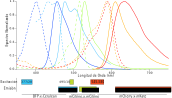
\includegraphics[width=0.9\textwidth]{img/cap_3/fluospectra.pdf}
    \caption{\footnotesize{Espectros de excitación y emisión de los fluoróforos seleccionados. En la sección inferior se muestran los filtros de ecitación y emisión utilizados para cada par de fluoróforos. Si se hace una adquisición secuencial no es necesario corregir sangrado espectral entre canales. Adaptado de \cite{Corbat2018}.}}
    \label{fig:fluospectra}
\end{figure}

Habiendo identificado los pares de fluoróforos con mayor rango dinámico en anisotropía de polarización, resta elegir la secuencia de unión entre ambos, en nuestro caso, la caspasa a la que será sensible. Debido a la facilidad con que se pueden intercambiar los pares y secuencias, se utilizaron varias combinaciones a lo largo de la tesis.

Desde un punto de vista evolutivo, la cascada apoptótica está bastante conservada. A lo largo de la evolución de caspasas, estas aumentaron en cantidad y funcionalidad dependiendo del organismo en cuestión. Aunque cada caspasa tiene especificidad por ciertas secuencias de aminoácidos, algunas caspasas comparten ésta especificidad. Por ejemplo, las caspasas efectoras 3 y 7 clivan en el dominio DEVD. Por otro lado, las caspasas iniciadoras 8 y 9 reconocen los sitios IETD y LEHD, respectivamente \citep{Sakamaki2009}. Sabiendo esto, las variantes se denominarán acorde a la caspasa siendo sensada y el color del par de fluoróforos utilizado. Siguiendo la denominación de las publicaciones sCasx-FP, donde x corresponde a la caspasa sensada: caspasa 3 para DEVD, caspasa 8 para IETD-IETD y caspasa 9 para LEHD; mientras que FP (por las siglas de \ening{fluorescent pair}) será reemplazado por RP, GP o BP según sea el par rojo, verde o azul, respectivamente (por sus siglas en inglés).

Los biosensores se construyeron insertando el segundo fluoróforo amplificado por PCR y delimitado por los sitios de restricción de Spe1 y Sal1 y conteniendo un codón STOP en los sitios de restricción Spe1/Sal1 de un vector-C1 (Clontech). Adicionalmente, el producto de PCR tenía una secuencia de unión en el extremo 5'. Estos plásmidos se utilizaron como controles no clivables. Por otro lado, para construir los sensores clivables por la caspasa, se utilizaron las secuencias que codificaban para los sitios de clivado de las caspasas amplificadas por PCR y delimitadas por sitios de restricción BSP1 y Spe1, y luego subclonados a los sitios de restricción correspondientes en los plásmidos de control no clivables, volviéndolos plásmidos que codifican para el sensor clivable.


%%%%%%%%%%%%%%%%%%%%%%%%%%%%
\section{Estimación de la Anisotropía del Dímero y del Monómero}


Para poder estimar la actividad de la caspasa a partir de las curvas de anisotropía es necesario estimar los valores de anisotropía del monómero y dímero de cada par de fluoróforos. Para ello, se tomaron las curvas medidas experimentalmente y se seleccionó mediante máscaras la región correspondiente al momento en que transcurre la apoptosis. Se tomó un promedio de los cinco valores de anisotropía previos al inicio de la máscara y posteriores para estimar la anisotropía del dímero y monómero, respectivamente. Dado que los valores estimados para cada curva tenían mucha variabilidad, y considerando las fuentes de error en su estimación (ver sección \ref{sec:matmet:CalculoAnisotropia}), se decidió estimar dichos valores para cada curva en lugar de utilizar un único valor para cada par de biosensores. De todas formas, se corroboró que en todos los casos la diferencia de anisotropía era positiva y de un valor distinguible del ruido experimental (ver \cref{fig:anisotropy_histogram}).

\begin{figure}
    \centering
    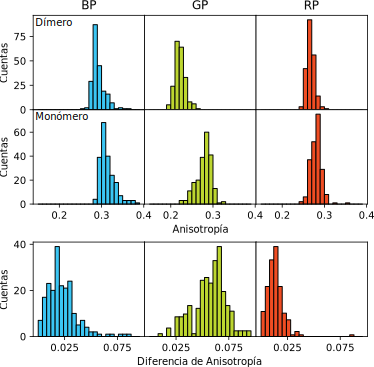
\includegraphics[width=0.7\textwidth]{img/cap_3/anisotropy_histograms_all.pdf}
    \caption{\footnotesize{Histogramas correspondientes a las anisotropías del monómoero y dímero estimadas a partir de 212 curvas. Para cada biosensor, los histogramas de la anisotropía del dímero y monómero se superponen bastante, mientras que en los histogramas de las diferencias se ve que todos los valores son positivos. Adaptado de \cite{Habif2021}.}}
    \label{fig:anisotropy_histogram}
\end{figure}


%%%%%%%%%%%%%%%%%%%%%%%%%%%%
\section{Calibración del Parámetro \texorpdfstring{$\Delta b$}{Deltab}}


Habiendo seleccionado los pares de fluoróforos a utilizarse, debemos hallar el valor de $\Delta b$ correspondiente a cada par. La calibración más directa que a uno se le puede ocurrir es obtener los valores de brillo por cada tipo de molécula para determinar así los valores de $b$ y $\Delta b$. Sin embargo, esto no siempre es posible ni la mejor forma. Otra posibilidad consiste en generar biosensores con los tres pares de fluoróforos pero que sensen la misma caspasa. Como la caspasa no tiene ninguna preferencia por ninguno de los tres sensores, las curvas de los tres deberían corresponder a curvas de actividad idénticas, así como la diferencia entre los máximos de actividad debería ser nula.

\begin{figure}
    \centering
    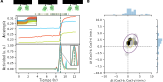
\includegraphics[width=0.9\textwidth]{img/cap_3/onecasp.png}
    \caption{\footnotesize{Se transfectaron a células HeLa los biosensores sCas3-RP, sCas3-GP y sCas3-BP y se las estimuló con staurosporina (N=54). Adaptado de \cite{Corbat2018}. \textbf{A.} Se muestra a modo de ejemplo tres curvas de anisotropía con sus correspondientes curvas de actividad. En la sección superior cada varilla representa el instante de máxima actividad observado para alguna de las 54 células analizadas. Todas las curvas de anisotropía se graficaron superpuestas en el recuadro superior, mientras que el recuadro inferior contiene una sección amplificada de la región de los máximos. \textbf{B.} Histograma bidimensional en donde se muestran las diferencias de tiempo entre los biosensores en forma de hexágonos. Las curvas de nivel se obtienen de un gráfico de estimación de densidad de kernel y encierran el 34\% (amarillo) y 68\% (violeta) de los datos. El gráfico superior y derecho son las distribuciones marginales de las diferencias de tiempo.}}
    \label{fig:onecasp}
\end{figure}

Para calibrar los pares de fluoróforos utilizados, se transfectaron a las células los sensores sCas3-RP, sCas3-GP y sCas3-BP. Para inducir apoptosis, se utilizó una concentración 1~$\mu$M de staurosporina. Siguiendo el protocolo experimental delineado en el \cref{cap:MatMet}, se obtuvieron y analizaron las sucesivas imágenes tomadas en un lapso de 15~hr. A partir de las curvas de anisotropía generadas, se estimaron las correspondientes curvas de actividad de la caspasa y se recuperó para cada una el tiempo de máxima de actividad (ver \cref{fig:onecasp}A). A continuación, se buscaron los valores de $\Delta b$ que minimicen las diferencias entre tiempos de máxima actividad, obteniéndose 0.15 para BP, 0.17 para GP y -0.15 para RP. Se presenta un histograma bidimensional en la \cref{fig:onecasp}B de los valores de los tiempos obtenidos.


%%%%%%%%%%%%%%%%%%%%%%%%%%%%
\section{Perturbación de los Biosensores}


Hasta ahora hemos modelado e imaginado a los biosensores y sus caspasas separadas en un modelo simple, pero en realidad, éstas son parte de una cascada de señalización dentro de la célula y los sensores son añadidos de forma exógena. Como cualquier especie agregada, ésta competirá por la enzima con las especies endógenas y propias del sistema. Esto quiere decir que la propagación de la señal a través de la red puede verse demorada por un efecto de secuestro de las caspasas por parte de los biosensores. Este efecto se torna más importante ya que depende de la concentración y los biosensores transfectados se hallan en concentraciones elevadas debido a que el promotor viral (CAG) hace que sean sintetizados constantemente \citep{Wachsmuth2015}. 

Al transfectar cada biosensor en un plásmido distinto, cada uno tiene cierta probabilidad de ser efectivamente incorporado a la célula \citep{Schwake2010}. Esto se traduce en que habrán células transfectadas con uno o dos de las variantes de biosensores en lugar de los tres, así como células que tendrán uno en exceso y los otros biosensores en menor concentración. Este fenómeno combinado con el efecto de secuestro de cada biosensor se traduce en que la demora introducida en cada nodo sensado de la red será distinta de célula a célula, dependiendo de como fue la transfección.

Surgieron varias estrategias para mejorar la co-expresión de proteínas: desde utilizar múltiples promotores \citep{Kriz2010}, promotores bidireccionales \citep{Vogl2018}, sitios internos de entrada al ribosoma (IRES por sus siglas en ingles, \cite{Wong2002}) o el uso de secuencias virales de péptidos 2A \citep{Kim2011}. Aunque utilizar múltiples promotores asegura una expresión elevada de los genes transfectados, no asegura la estequiometría en la expresión. Los promotores bidireccionales traen aparejada la dificultad de su construcción así como su cantidad limitada de genes. Por otro lado, las secuencias de IRES suelen tener más de 800 pares de bases y es sabido que secuencias muy extensas traen aparejados otros problemas al momento de expresarse. Por último, las secuencias virales 2A emergieron en la última década y consisten en secuencias \textit{auto-clivables} de alrededor de 20 aminoácidos. 

El mecanismo por el cual las secuencias 2A se clivan es un evento de hidrólisis co-transduccional entre los residuos de glicina y prolina de una secuencia conservada (Asp-Val/Ile-Glu-X-Asn-Pro-Gly-¯-Pro), dando lugar a la expresión de proteínas distintas a partir de un único ARN mensajero. Específicamente, se impide la formación de una unión peptídica normal vía un ``salto ribosomal'' sin afectar la traducción de la proteína codificada río abajo \citep{Szymczak2005}. En el trabajo de \cite{Szymczak2004}, se utiliza un plásmido multicistrónico codificando para las cuatro subunidades del complejo CD3 y así restaurar el desarrollo de células T en ratones deficientes de dicho complejo. Además de ser útiles para expresar subunidades de complejos, pueden ser implementadas para expresar diversos reporteros como muestran \cite{Levin2014} al utilizarlas para expresar una proteína fluorescente, una luciferasa para detección mediante bioluminiscencia y una quinasa de timidina para poder visualizarla a través de tomografía de emisión de positrones.

Luego de haber identificado el impacto de la concentración de los biosensores, se comenzó el diseño de una estrategia para controlar la estequiometría de los biosensores. La caracterización de dicha implementación fue realizada en conjunto con el Dr. Martín Habif en el Laboratorio de Electrónica Cuántica; y en viajes que realizamos al Instituto Pasteur de Montevideo (Uruguay) y Max Planck Institute for Molecular Physiology (Dortmund, Alemania). A continuación, se trabajo en conjunto para estudiar el efecto de dicha modificación en la variabilidad de los observables biológico y analizar los datos de todos los experimentos realizados.


%%%%%%%%%%%%%%%%%%%%%%%%%%%%
\section{Construcción de CASPAM}


Con el objetivo de reducir la variabilidad en la estequiometría de los sensores y basándonos en el trabajo de \cite{Goedhart2011}, donde se muestra que utilizar secuencias virales 2A resulta en una mayor correlación en la concentración de dos fluoróforos, se implementó un plásmido multicistrónico donde cada biosensor se halla separado por dichas secuencias. Para su confección, se tomaron los tres sensores de actividad caspasa (CAS, por sus siglas en inglés) y se los arregló en tandem utilizando secuencias flexibles (GGGSGGG) y virales 2A (P2A: \seqsplit{ATNFSLLKQAGDVEENPGP} y T2A: \seqsplit{EGRGSLLTCGDVEENPGP}) entre ellos. La elección de las secuencias estuvo guiada por el trabajo de \cite{Liu2017} donde muestran como la eficiencia de auto-clivaje decrece en el orden P2A\textless T2A\textless E2A\textless F2A. Se reemplazaron todos los codones STOP con glicina a excepción del fluoróforo ubicado en el extremo 3' del constructo. Finalmente, el gen sintético de $\sim$5kb fue clonado entre los sitios de restricción KpnI/EcoRI de un vector pcDNA3.1(+) (Life Technologies, Grand Island, NY). La combinación de sensores seleccionados fue sCas3-GP, sCas8-BP y sCas9-RP y el control de la traducción está regido por un promotor de Citomegalovirus (CMV). La integridad de cada cassette en mCitrine-DEVD-mCitrine-P2A-tagBFP-IETD-Cerulean-T2A-mCherry-LEHD-mKate fue confirmada por secuenciación en el constructo final. Considerando que los tres biosensores pueden ser multiplexados mediante anisotropía de polarización, se nombró al constructo CASPAM, por sus siglas en inglés \textit{Caspase Activity Sensor by Polarization Anisotropy Multiplexing} (ver \cref{fig:secuencia}).

\begin{figure}[htb]
    \centering
    \includegraphics[width=0.7\textwidth]{img/cap_3/CASPAM_seq.pdf}
    \caption{\footnotesize{Secuencia de CASPAM. Se pueden apreciar los tres biosensores sCas3-GP, sCas8-BP y sCas9-RP separados por secuencias virales 2A y secuencias flexibles compuestas por GGGSGGG. Adaptado de \cite{Habif2021}.}}
    \label{fig:secuencia}
\end{figure}

Luego, se verificó la expresión de los biosensores a partir de la transfección de CASPAM en células HeLa. Una vez transfectadas, se las incubó por 24~hr y se las sometió a Western Blot. Este procedimiento permite inferir a partir de la distancia recorrida desde su punto de siembra el peso molecular de la proteína de interés. El no haber detectado bandas en las regiones de peso molecular equivalente al de tres biosensores ($\sim$170~kD) ni dos biosensores ($\sim$110~kD) confirma que no se hallan subproductos correspondientes a un clivaje incompleto entre biosensores (ver \cref{fig:transfeccion}A). Contrario a esto, se pudo apreciar una banda intensa correspondiente al peso molecular de un dímero de fluoróforos ($\sim$52~kD), que además confirma que no se hallan biosensores clivados por caspasas en condiciones sin perturbar.

\begin{figure}
    \centering
    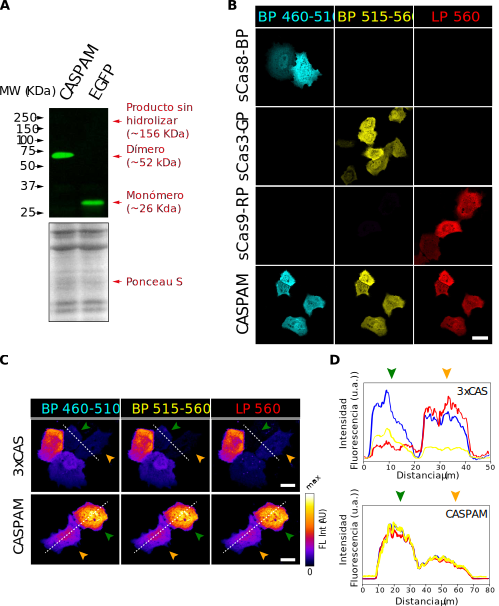
\includegraphics[width=0.8\textwidth]{img/cap_3/transfeccion.pdf}
    \caption{\footnotesize{Se transfectaron células HeLa con CASPAM y se corroboró la síntesis de los biosensores. Adaptado de \cite{Habif2021}. \textbf{A.} Se realizó un Western Blot y se lo marcó con anticuerpos anti-GFP. Éstos anticuerpos se pueden visualizar mediante fluorescencia y se unen tanto a GFP como a mCitrine y CFP. Se puede apreciar que en el carril de células transfectadas con EGFP se ve una única marca correspondiente a un único fluoróforo, mientras que en las células transfectadas solo se ve una marca en el doble de peso molecular. Al no verse marcas en tamaños mayores, interpretamos que no hay productos sin hidrolizar. En la imagen inferior se ve una tinción con Ponceau S que sirve para estimar pesos moleculares sin afectar las proteínas del gel. \textbf{B.} Células transfectadas con los tres sensores por separado o con CASPAM y luego fijadas fueron analizadas por microscopía confocal. Se puede apreciar que no hay sangrado espectral entre los distintos canales, así como que las células transfectadas con CASPAM expresan lo tres biosensores. \textbf{C.} Imágenes de microscopía confocal de las células transfectadas con 3xCAS y CASPAM. Los perfiles de intensidad de las rectas se muestran en \textbf{D}. Aunque las intensidades de los biosensores transfectados con CASPAM varían de célula a célula, éstos no varían tanto entre canales de la misma célula. En contraposición, las células transfectadas con 3xCAS presentan una elevada variabilidad en la intensidad intercanal e intercelular.}}
    \label{fig:transfeccion}
\end{figure}

Más allá de de la presencia de los biosensores dentro de las células, se corroboró por medio de microscopía de fluorescencia que los tres biosensores se encuentren en células únicas y que su plegado sea el correcto, dando lugar a emisión de fluorescencia. Para ello se transfectaron células HeLa con una mezcla de plásmidos codificando para 3 CAS (sCas3-GP, sCas9-BP, sCas8-RP) o con CASPAM y se las fijó con paraformaldehído 24~hr después. Se utilizó microscopía confocal para observar la emisión de los fluoróforos en los distintos canales, y como se esperaba, no se detectó ningún sangrado entre ellos (ver \cref{fig:transfeccion}B). Adicionalmente, las células transfectadas con CASPAM no sólo mostraban fluorescencia en los debidos canales, sino que también mostraban muy poca variabilidad en intensidad intercanal aunque sí variabilidad intercelular. Esto sugiere que la estequiometría entre los biosensores esta mejor conservada al utilizar CASPAM (ver \cref{fig:transfeccion}C y D).


%%%%%%%%%%%%%%%%%%%%%%%%%%%%
\section{Caracterización de la Expresión de CASPAM}


A continuación, se utilizó citometría de flujo para caracterizar los niveles de fluorescencia de una gran población de células (FACS) y espectroscopia de correlación de fluorescencia (FCS) para poder determinar adecuadamente la estequiometría. FACS consiste en hacer pasar del orden del miles de células de a una por un sistema óptico que permite clasificar y caracterizar cada una según sus propiedades ópticas y de fluorescencia. En cuanto a FCS, es una técnica basada en microscopía confocal de detección de molécula única donde se analizan las correlaciones en fluctuaciones de intensidad generadas por partículas fluorescentes entrando y saliendo de un volumen de observación del orden de un femtolitro \citep{Digman2008}. Cabe destacar que FACS es una técnica extensiva en cuanto a que describirá miles de células, mientras que FCS requiere varias repeticiones de la medición de cada punto por lo que no es posible describir tantas células. Otra diferencia importante es el rango dinámico de cada una, ya que FACS puede reportar niveles de fluorescencia con varios ordenes de magnitud de diferencia, mientras que FCS depende de los parámetros microscopio utilizado y es mucho menor. Para ambos experimentos, se transfectaron nuevamente células HeLa con 3xCAS y CASPAM y se analizaron 24~hr post transfección. Además, FACS refiere a la fluorescencia detectada en cada célula y por lo tanto su relación no nos brinda información sobre cual es la estequiometría, sino cuanto varía ésta entre células. A partir de FCS podemos estimar la cantidad de moléculas dentro del volumen confocal y así calcular la estequiometría entre los sensores.


\subsection{Clasificación de Células por Fluorescencia Activada}


Además de las células transfectadas con 3xCAS y CASPAM, se analizaron células transfectadas con: i) sCas3-GP, ii) sCas8-RP, iii) sCas9-BP, iv) sCas3-GP + sCas8-RP, v) sCas3-GP + sCas9-BP, vi) sCas8-RP + sCas9-BP. Se utilizó un citómetro FACS-Aria Fusion (BD Biosciences) equipado con láseres de 405~nm, 488~nm y 561~nm. Se cuantificó la emisión de fluorescencia utilizando los filtros BP450/50 (verde), BP530/30 (azul) y BP610/20 (rojo). Para cada muestra se dejó pasar un total de $2 \times 10^4$ cuentas en gráfico de puntos de forward scatter (FSC) versus side scatter (SSC), excluyendo dobletes. Los datos se adquirieron por medio de CellQuest software (BD Biosciences) y se procesaron con FlowJo v7.6.5 software.

Los análisis de FACS de células transfectadas con un vector vacío y con un único plásmido que codifique para un único biosensor sirvieron de calibración (ver \cref{fig:FACS_singles}). Los niveles de fluorescencia detectados en las células que fueron transfectadas con el vector vacío se corresponden con autofluorescencia y el offset de detección (ver \cref{fig:FACS_singles}A). Por otro lado, las células transfectadas con cada uno de los biosensores sirven para denotar las regiones de intensidad en las que se detectarán cada uno de los pares de fluoróforos. Además, podemos apreciar que no se detecta fluorescencia en los canales correspondientes a los biosensores no transfectados. En los casos de las células transfectadas con plásmidos para dos biosensores, no muestran señal en el canal del biosensor faltante (\cref{fig:FACS_dobles}).

\begin{figure}
    \centering
    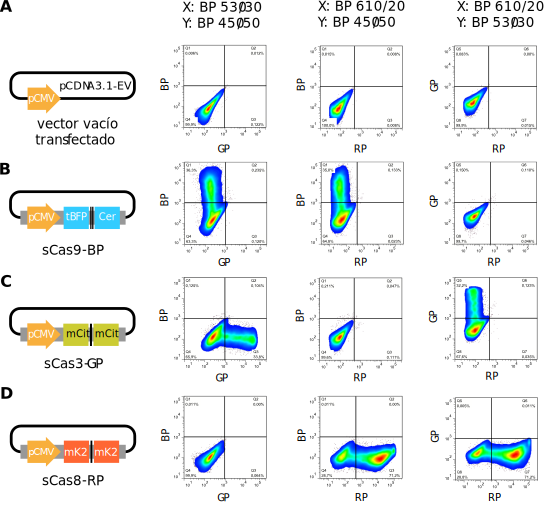
\includegraphics[width=0.9\textwidth]{img/cap_3/FACS_singles.pdf}
    \caption{\footnotesize{Se transfectaron células HeLa con un vector vacío (\textbf{A}), sCas9-BP (\textbf{B}), sCas3-GP (\textbf{C}) y sCas8-RP (\textbf{D}). En células transfectadas con un vector vacío se puede apreciar un bajo nivel de fluorescencia detectados que corresponde a autofluorescencia. En los casos de transfecciones con un único biosensor, sólo se ve un mínimo de fluorescencia correspondiente a autofluorescencia y una región intensa en el canal del biosensor transfectado, pero no en otros canales. Adaptado de \cite{Habif2021}.}}
    \label{fig:FACS_singles}
\end{figure}

\begin{figure}
    \centering
    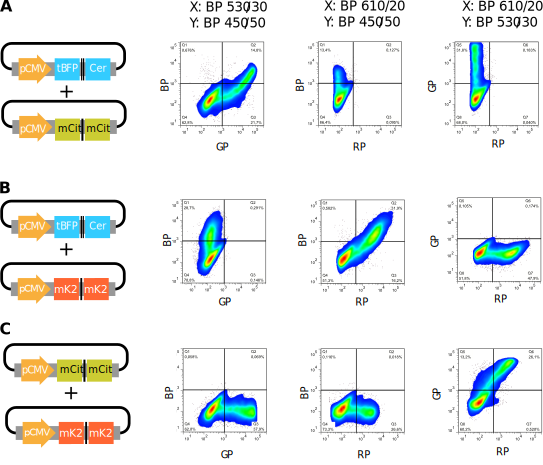
\includegraphics[width=0.9\textwidth]{img/cap_3/FACS_dobles.pdf}
    \caption{\footnotesize{Se transfectaron células HeLa con los pares de plásmidos que codifican para los biosensores: sCas3-GP + sCas9-BP (\textbf{A}), sCas3-GP + sCas8-RP (\textbf{B}) y sCas8-RP + sCas9-BP (\textbf{C}). FACS correspondiente a células transfectadas con dos biosensores en las que sólo se ve un mínimo de fluorescencia correspondiente a autofluorescencia y una región intensa que cruza entre los canales de ambos biosensores transfectados, pero no en el canal del biosensor remanente. Adaptado de \cite{Habif2021}.}}
    \label{fig:FACS_dobles}
\end{figure}

Se puede apreciar que la heterogeneidad en la expresión relativa de cada biosensor es mucho mayor en el caso de las células transfectadas con 3xCAS que con CASPAM (ver \cref{fig:FACS}). En el caso de 3xCAS, se pueden encontrar subpoblaciones que expresan sólo uno o dos sensores. Por otro lado, la relación entre las emisiones de las células transfectadas con CASPAM se conserva a lo largo de todo el rango dinámico. Aunque es sabido que la eficiencia de transfección puede mejorarse modificando el protocolo utilizado, sólo el 68,25\% las células transfectadas con 3xCAS expresaron todos los biosensores, mientras que 15,77\% expresaron sólo dos, y las restantes 15,97\% un único biosensor. En contraposición, la totalidad de las células transfectadas con CASPAM expresaron los tres biosensores (ver \cref{fig:FACS}B). Se utilizó un análisis de correlación múltiple de Pearson para cuantificar la correlación entre las intensidades detectadas obteniéndose r$_{R,GB}$=0.455, r$_{B,GR}$=0.566 y r$_{G,BR}$=0.572 para 3xCAS, mientras que para CASPAM, r$_{R,GB}$=0.962, r$_{B,GR}$=0.962 y r$_{G,BR}$=0.959, mostrando así una mejor correlación (ver \cref{fig:FACS}C). En resumen, CASPAM no solo logra coexpresar todos los biosensores, sino que también consigue un razón de coexpresión más conservada entre células.

\begin{figure}[t!]
    \centering
    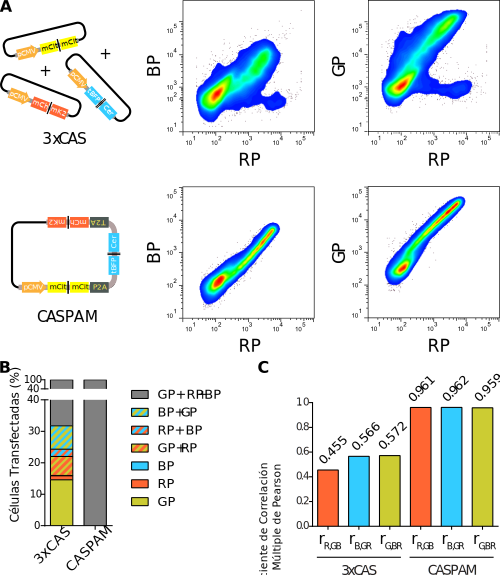
\includegraphics[width=0.8\textwidth]{img/cap_3/FACS.pdf}
    \caption{\footnotesize{Se transfectaron células HeLa con CASPAM y 3xCAS para estudiar la coexpresión a través de FACS. Adaptado de \cite{Habif2021}. \textbf{A.} En la sección superior se pueden ver los resultados del FACS en células transfectadas con 3xCAS. Además de una elevada variabilidad en la fluorescencia en la región correspondiente a células que expresan los tres biosensores, se pueden apreciar lóbulos correspondientes a células que no expresan todos los biosensores. Sin embargo, en el caso de células transfectadas con CASPAM (sección inferior), se aprecia una elevada correlación en la intensidad de fluorescencia y no se encuentran lóbulos correspondientes a células que no expresen alguno de los biosensores. \textbf{B.} Se estimó mediante ventaneo (gating) de las regiones del FACS que porcentaje de células transfectadas expresaban qué biosensores. Se vio que todas las células transfectadas con CASPAM expresaban los tres biosensores, mientras que sólo el 68,25\% las células transfectadas con 3xCAS expresaron todos los biosensores, 15,77\% expresaron sólo dos, y las restantes 15,97\% un único biosensor. \textbf{C.} Se calculó el coeficiente de correlación múltiple de Pearson para cada biosensor en ambos tipos de transfección. Se puede ver que en el caso de CASPAM, la correlación es considerablemente mayor.}}
    \label{fig:FACS}
\end{figure}


\subsection{Espectroscopia de Correlación de Fluorescencia}


\begin{figure}[b!]
    \centering
    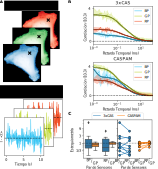
\includegraphics[width=0.8\textwidth]{img/cap_3/FCS.pdf}
    \caption{\footnotesize{Se transfectaron células HeLa con 3 CAS por separado y con CASPAM y se analizó la estequiometría de la síntesis de los biosensores. Adaptado de \cite{Habif2021}. \textbf{A.} Se analizaron 10 células de las que se adquirieron 10 repeticiones de 10 segundos de las fluctuaciones de un único punto. Como se evidencia en las figuras inferiores, no se apreció una deriva de la señal. \textbf{B.} Se calcularon las funciones de autocorrelación de cada repetición adquirida y se promediaron todas las correspondientes a un mismo punto y un mismo canal. Luego se ajustaron todas las curvas con un modelo de difusión corregido por estado triplete y se obtuvieron así los valores de G(0) y coeficientes de difusión, entre otros parámetros. \textbf{C.} Se calcularon las relaciones de concentración entre los pares de biosensores. La varianza de las relaciones de las células transfectadas con CASPAM es mucho menor que la de 3xCAS. Para  3xCAS, el intervalo intercuartil de estequiometría entre BP y GP fue de 0.47-1.79, y 0.28-1.86 para RP y GP, mientras que para CASPAM la estequiometría entre BP y GP estuvo entre 0.58-1.01 y 0.83-1.11 para RP y GP.}}
    \label{fig:FCS}
\end{figure}

En este caso se utilizó un microscopio invertido confocal de escaneo Leica TCS SP8 equipado con un láser de luz blanca pulsado de 470-670~nm (WLL2 Kit, NKT Photonics) que tenía montada una cámara de ambiente controlado (Life Imaging Services) que mantenía la temperatura a 37$^{\circ}$C. Las células se hallaban inmersas en medio DMEM (con 25~mM HEPES y sin rojo fenol). Se utilizó un objetivo HC PL APO 63x/1.4 NA CS2 de inmersión en aceite (Leica Microsystems). Las fluctuaciones de fluorescencia se obtuvieron mediante escaneo de un único punto en 10 repeticiones de 10 segundos (ver \cref{fig:FCS}A). Se calcularon las funciones de autocorrelación para cada repetición y luego se promediaron todas las funciones correspondientes a un mismo punto y canal. Para caracterizar el volumen confocal se utilizaron microesferas fluorescentes TetraSpeck de 100~nm (Invitrogen).

Se utilizó un modelo de difusión corregida por estado triplete para ajustar las funciones de autocorrelación promediadas. Dicha ecuación consiste en

\begin{equation}
    G (\tau) = G(0) \frac{(1 - F + F e^{-\tau/\tau_F})}{(1-F)} \frac{1}{(1 + (\tau / \tau_{D})) (1 + a^{-2} (\tau / \tau_{D}))^{1/2}} + G(\infty),
\end{equation}

\noindent donde $\tau$ es el retardo temporal en la autocorrelación,$\tau_D$ es el tiempo característico de difusión, $a$ es la razón $\omega_z / \omega_{xy}$ entre radio axial y lateral, $F$ es la proporción de partículas que entran en estado triplete, dejando de fluorescer, y $\tau_F$ su tiempo de relajación \citep{Widengren1995}. A partir de $G(0)$ se puede calcular la cantidad de difusores en el volumen a través de

\begin{equation}
    G(0) = \frac{1}{<N>} = \frac{1}{V_{Eff} <C>},
\end{equation}

\noindent y luego su concentración.

A partir de los ajustes, se analizaron los tiempos característicos de difusión así como la concentración de cada biosensor en cada célula. En cuanto a tiempos de difusión, aunque los volúmenes son levemente distintos entre canales, no se pudo apreciar una diferencia. Sin embargo, las concentraciones de biosensores variaban de canal a canal, así como de célula a célula. A pesar del rango dinámico considerablemente menor de FCS respecto a FACS, las células transfectadas con 3xCAS mostraron una variabilidad mucho más elevada que las transfectadas con CASPAM en la expresión relativa entre sensores (ver \cref{fig:FCS}C). En particular, para  3xCAS, la estequiometría entre BP y GP se mantuvo entre 0.47-1.79, y 0.28-1.86 para RP y GP, mientras que para CASPAM la estequiometría entre BP y GP estuvo entre 0.58-1.01 y 0.83-1.11 para RP y GP (donde los valores representan el rango intercuartil). Adicionalmente, la mediana de la expresión relativa entre cada par de biosensores de CASPAM fue cercana a la equimolaridad: 0.82 para BP y GP y 1.03 para RP y GP. Todo esto apunta a que CASPAM puede ser utilizado para obtener una co-expresión con un razón más definida entre biosensores en células individuales.


%%%%%%%%%%%%%%%%%%%%%%%%%
\section{Variabilidad en la Perturbación Introducida}


Habiendo caracterizado las mejoras introducidas por CASPAM en el control de la estequiometría, debemos corroborar dicha mejora en un experimento relevante para la biología. Para ello, se utilizaron nuevamente células transfectadas con 3xCAS o CASPAM, se las trató con staurosporina para inducir apoptosis y se las siguió mediante microscopía por 15~hr. Se analizaron las imágenes siguiendo el protocolo detallado en el capítulo \ref{cap:MatMet} y se obtuvieron los tiempos de máxima actividad de cada caspasa.

Como se discutió previamente, elevar la concentración del biosensor de alguna caspasa introducirá una demora en la propagación de la señal en la red. A modo de ejemplo, podemos tomar el modelo introducido en \cite{Corbat2018} (que será descripto en detalle en el capítulo \ref{cap:Modelos}) basado en ecuaciones diferenciales ordinarias y simular la cascada apoptótica utilizando concentraciones cada vez más altas de sCas3 (ver \cref{fig:variabilidad}A). Podemos apreciar que cambiando dicha concentración, la diferencia de tiempo entre máxima actividad de cada caspasa varía (ver \cref{fig:variabilidad}B). En la contraparte experimental, estudiaremos el impacto de seleccionar células cuya intensidad esté en un rango predefinido. Seleccionaremos células cuyo z-score de intensidad se encuentre entre -0.5 y 0.5 en cada biosensor. En efecto, debido a la elevada correlación entre la razón de intensidad de biosensores en las células transfectadas con CASPAM, seleccionar un rango de intensidad para un biosensor equivale a seleccionar un rango para los otros biosensores, a diferencia de las células transfectadas con 3xCAS. Luego de analizar el desvío estándar de las diferencias de tiempo entre los máximos de las caspasas, podemos apreciar que para CASPAM es considerablemente menor verificándose así una variabilidad menor en la perturbación introducida.

\begin{figure}[htb]
    \centering
    \includegraphics[width=0.9\textwidth]{img/cap_3/variabilidad.png}
    \caption{\footnotesize{Se simuló y se midió experimentalmente el efecto de introducir los biosensores con relación de estequiometría variables. Adaptado de \cite{Habif2021}. \textbf{A.} Se simularon curvas de actividad variando la concentración del biosensor sCas3 a lo largo de los valores utilizados en el modelo. La curva remarcada corresponde a la simulación con la mediana de concentración de sCas3, mientras que la región pintada engloba todas las curvas obtenidas. \textbf{B.} Se graficó la diferencia de tiempo entre los máximos de actividad de las caspasas 9 y 3 y las caspasas 8 y 9 para cada concentración de sCas3 simuladas. \textbf{C.} Se estimó la fluorescencia de cada célula transfectada con CASPAM o 3xCAS y se graficaron los z-score de cada biosensor en función de los otros. Aunque el rango dinámico de microscopía es considerablemente menor que el de FACS, todavía se aprecia una variabilidad más elevada en las células transfectadas con 3xCAS. Luego se seleccionaron 3 grupos correspondientes a los que tenían una fluorescencia cuyo z-score se hallase entre -0.5 y 0.5. \textbf{D.} Se analizó el desvió estándar de las diferencias de tiempo entre los máximos de actividad de cada caspasa y se puede ver que en todos los casos CASPAM tiene menos variabilidad en los observables que 3xCAS. Esto se debe a que al seleccionar células en cierto rango de intensidad para un biosensor de CASPAM, se seleccionan células en un rango similar en los otros biosensores, mientras que esto no sucede en 3xCAS.}}
    \label{fig:variabilidad}
\end{figure}

Dentro de todo, CASPAM permite alcanzar una expresión casi equimolar de todos los biosensores, reduciendo así la variabilidad de las perturbaciones introducidas y, por ende, los observables biológicos. Adicionalmente, conocer la concentración relativa entre los biosensores introducidos facilitará el modelado del sistema ya que reduce la cantidad de parámetros a determinar. Desde un punto de vista experimental, al utilizar CASPAM no es necesario corroborar la expresión en todos los canales ya que la totalidad de las células que expresan un biosensor, expresan los otros dos. Además, es posible seleccionar los parámetros de adquisición buscando las células más intensas en un canal y utilizándolas para verificar los parámetros en los otros canales.


%%%%%%%%%  Modelos
\chapter{Dinámica de la Red de Caspasas}
\label{cap:Modelos}


La cascada apoptótica debe integrar información proveniente del entorno, a través de ligandos de la muerte o señales de supervivencia, con información del estado interno celular, como daño al ADN y estado de oxidación, para decidir si proceder con el programa de muerte celular. Para comprender la forma en que la red sopesa dicha información es necesario confeccionar un modelo que incluya los distintos módulos y poder contrastarlo con varios experimentos. En este capítulo presentaré el desarrollo de los modelos utilizados para describir el comportamiento del sistema bajo estudio. Comenzaré describiendo un modelo introducido en \cite{Corbat2018} que describe adecuadamente la dinámica de la red ante estímulos extrínsecos. Al detectar incongruencias entre las predicciones del modelo y los experimentos con estímulos intrínsecos, se encontró una retroalimentación faltante y se completó el modelo. Éste último fue presentado en \cite{Corbat2021} y se comprobó que además de describir la dinámica ante estímulos intrínsecos y extrínsecos, podía predecir resultados de experimentos previos de otros laboratorios.


%%%%%%%%%%%%%%%%%%%%%%%%%%%%%%%
\section{Adquisición del Cuerpo de Datos}


Siguiendo el protocolo descripto en el capítulo \ref{cap:MatMet}, se transfectaron células con los biosensores caracterizados en el capítulo \ref{cap:Biosensores} y se las estimuló con TNF-$\alpha$ o staurosporina, estímulos extrínseco e intrínseco respectivamente \citep{Sakamaki2009, Malsy2019}. Dado que en este caso contamos con tres biosensores de espectro distinto, la secuencia de adquisición de imágenes tuvo que ser modificada. Se incluyeron los canales rojo y azul, utilizándose 150~ms de exposición ya que la eficiencia de detección es menor en esos rangos. Es necesario considerar el tiempo necesario para cambiar de canal que es de 500~ms, demorándose 1.6~s en adquirir las imágenes correspondientes a los tres canales con sus respectivas dos polarizaciones (ver \cref{fig:tiempo_adq_tres_canales}). Nuevamente, se estimó que es posible adquirir imágenes correspondientes a 75 posiciones como mínimo antes de volver a la primer posición, manteniendo 5 minutos de resolución temporal. Esto correspondería a 1125 a 3000 células por experimento realizado.

\begin{figure}
    \centering
    \includegraphics[width=0.7\textwidth]{img/cap_4/tiempo_adq_tres_canales.pdf}
    \caption{\footnotesize{Esquema de los tiempos característicos de la adquisición secuencial de imágenes para cada canal y en cada polarización. En este caso se usaron 50~ms de tiempo de exposición para adquirir cada imagen del canal verde y 150~ms para cada una de los canales rojo y azul, 90~ms entre cada polarización y 500~ms para alternar entre canales. La platina motorizada necesita 2 segundos para cambiar de posición y entrar en foco. El tiempo necesario para cambiar la configuración de canal está incluido en el tiempo necesario para que la platina se traslade de una posición a otra.}}
    \label{fig:tiempo_adq_tres_canales}
\end{figure}

\begin{figure}[htb]
    \centering
    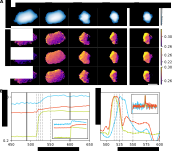
\includegraphics[width=0.8\textwidth]{img/cap_4/cels_anis.pdf}
    \caption{\footnotesize{Ejemplo ilustrativo del análisis de anisotropía. Adaptado de \cite{Habif2021}. \textbf{A.} Imágenes de fluorescencia y anisotropía de cada canal para una célula apoptótica. Se puede apreciar el aumento de anisotropía a distintos tiempos en cada canal. Cabe destacar que estas imágenes se generaron a modo ilustrativo y no fueron utilizadas para calcular las curvas de anisotropía. \textbf{B.} Curvas de anisotropía calculadas para la célula mostrada en \textbf{A}. El recuadro muestra la curva de anisotropía completa, las líneas verticales a trazos marcan los tiempos correspondientes a las imágenes, mientras que los rebordes oscuros corresponden a la sección de actividad graficada a la derecha.}}
    \label{fig:cels_anis}
\end{figure}

A partir del análisis de las imágenes, se obtuvieron las curvas de anisotropía para cada sensor en cada célula (ver \cref{fig:cels_anis} y \cref{fig:curvas_experimentales}). Luego, se generó un cuerpo de datos que contenía los tiempos de máxima actividad de las caspasas de las vías efectora, intrínseca y extrínseca de las 335 células apoptóticas, 152 estimuladas extrínsecamente y 183 de forma intrínseca. Como se mostró en la sección \ref{sec:Observable}, el tiempo de máxima actividad de cada caspasa sirve de referencia al tiempo de activación (ver \cref{fig:curvas_experimentales}). Es interesante notar que en ambos casos las caspasas extrínsecas y efectoras tienen un perfil sigmoideo, mientras que la intrínseca tiene un perfil hiperbólico.

\begin{figure}[htb]
    \centering
    \includegraphics[width=0.9\textwidth]{img/cap_4/all_experimental_curves.png}
    \caption{\footnotesize{Se transfectaron células HeLa con los biosensores de caspasas y se las expuso a estímulos extrínsecos e intrínsecos. \textbf{A.} Curva de anisotropía de ejemplo de una célula estimulada extrínsecamente. En este caso se utilizaron los sensores sCas3-BP, sCas8-RP y sCas9-GP. En el gráfico inferior se muestran las curvas de actividad obtenidas. Notar el perfil sigmoideo de las caspasas extrínsecas y efectoras, mientras que la intrínseca tiene un perfil hiperbólico. Adaptado de \cite{Corbat2018}. \textbf{B.} Curvas de anisotropía de ejemplo de una célula estimulada intrínsecamente. En este caso se utilizaron los sensores sCas8-BP, sCas9-RP y sCas3-GP. En el gráfico inferior se muestran las curvas de actividad obtenidas. Notar el perfil sigmoideo de las caspasas extrínsecas y efectoras, mientras que la intrínseca tiene un perfil hiperbólico. Adaptado de \cite{Corbat2021}.}}
    \label{fig:curvas_experimentales}
\end{figure}

Podemos apreciar una elevada variabilidad en el inicio de la cascada apoptótica, del orden de varias horas, utilizando el tiempo de máxima actividad de la caspasa efectora como referencia (ver \cref{fig:tiempos_experimentales}A). La diferencia entre los tiempos de activación de los distintos nodos es menos variable y del orden de minutos.  Luego, se calcularon las diferencias entre los tiempos de máxima actividad de las caspasas iniciadoras (caspasa 8 extrínseca y caspasa 9 intrínseca) y la efectora (caspasa 3). Se estimó un histograma de densidad utilizando funciones gaussianas para convolucionar con cada tiempo hallado (Kernel Density Estimation o KDE) y se graficaron las curvas de nivel que envolvían el 34\% y 68\% de los datos experimentales (ver \cref{fig:tiempos_experimentales}B). Podemos apreciar que prácticamente todos los tiempos, correspondientes a ambos estímulos caen en el primer cuadrante, lo que se traduce en que la caspasa efectora es la primera en alcanzar el máximo de actividad. En principio, uno esperaría que las caspasas iniciadoras sean las primeras en alcanzar el máximo de actividad, sin embargo, esto no ocurre debido a que éstas están fuertemente inhibidas y controladas. Una vez que la caspasa efectora alcanza el máximo de actividad, ésta retroalimenta a las iniciadoras, permitiéndoles alcanzar su máximo de actividad. Este mecanismo de inhibición de las iniciadoras y retroalimentación de la caspasa efectora evita que activaciones accidentales de caspasas iniciadoras desencadenen una respuesta completa. A su vez, si la caspasa efectora comenzará el proceso de apoptosis, la retroalimentación evitaría que pueda ser interrumpido culminando en una célula que sobrevive luego de haberse producido daño irreparable por parte de la caspasa efectora.

\begin{figure}[htb]
    \centering
    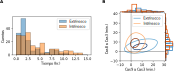
\includegraphics[width=0.9\textwidth]{img/cap_4/tiempos_experimentales.png}
    \caption{\footnotesize{Se estudiaron los tiempos de máxima actividad de cada caspasa y las relaciones entre ellos. De las 335 curvas apoptóticas, 152 correspondían a células estimuladas extrínsecamente y 183 a intrínsecamente estimuladas. Adaptado de \cite{Corbat2021}. \textbf{A.} Se confeccionaron histogramas del tiempo de máxima actividad de la caspasa efectora y se lo asoció con el inicio de la cascada apoptótica. Se pudo apreciar una elevada variabilidad, del orden de horas, en este desencadenamiento. \textbf{B.} Se analizaron las diferencias entre los tiempos de máxima actividad de las caspasas iniciadoras y la efectora. La caspasa efectora llega al máximo de actividad primera sin importar el estímulo utilizado. En el caso de células extrínsecamente estimuladas, la caspasa extrínseca 8 llegó al máximo de actividad $5_2^9$ minutos después que la caspasa efectora (mediana y rango intercuartil), mientras que la caspasa intrínseca 9 alcanza el máximo de actividad $8_5^{14}$ minutos después del máximo de actividad de la caspasa efectora. Al usarse estímulo intrínseco, la caspasa intrínseca fue la segunda en alcanzar el máximo de actividad $4_2^8$ minutos después de la efectora, mientras que la caspasa extrínseca lo alcanzó $9_5^{14}$ minutos después de la efectora.}}
    \label{fig:tiempos_experimentales}
\end{figure}

En el caso de células extrínsecamente estimuladas, la caspasa extrínseca 8 llegó al máximo de actividad $5_2^9$ minutos después que la caspasa efectora (mediana y rango intercuartil). Finalmente, la caspasa intrínseca 9 alcanza el máximo de actividad $8_5^{14}$ minutos después del máximo de actividad de la caspasa efectora. Por otro lado, al usarse estímulo intrínseco, la caspasa intrínseca fue la segunda en alcanzar el máximo de actividad $4_2^8$ minutos después de la efectora, mientras que la caspasa extrínseca lo alcanzó $9_5^{14}$ minutos después de la efectora. La distribución de puntos se ve afectada tanto por ruido en la determinación de los máximos de actividad, como por efecto de las demoras introducidas en los nodos por tener concentraciones distintas de biosensores y otras especies. Cabe destacar que el rango dinámico reducido de los sensores rojo y azul, hacen que la determinación de sus máximos sea más ruidosa (ver \cref{fig:tiempos_experimentales}).


%%%%%%%%%%%%%%%%%%%%%%%%%%%%%%%%%%%%
\section{Modelo de la Dinámica ante Estímulos Extrínsecos}


Se comenzó por estudiar y analizar distintos modelos en la bibliografía. \cite{Albeck2008} introdujeron en su trabajo un modelo que incluye los módulos extrínseco, intrínseco y efector con prácticamente todas las especies involucradas en la cascada (ver sección \ref{sec:intro:CascadaApoptotica} y \cref{fig:sketch_2018}). Considerando la completitud del modelo y el nivel de detalle que contiene, se decidió adaptarlo para incluir el comportamiento de los biosensores introducidos en el sistema. Para ello, se agregaron las especies correspondientes a cada biosensor en estado dimérico y se agregaron las reacciones por las cuales las caspasas se unen al biosensor y proceden a clivarlo.

\begin{figure}[htb]
    \centering
    \includegraphics[width=0.5\textwidth]{img/cap_4/model_simplified_noCas9FB.pdf}
    \caption{\footnotesize{Esquema simplificado del modelo de red de caspasas. Se pueden apreciar las ramas que intercomunican cada módulo. En particular, el módulo extrínseco activa el intrínseco y efector. El módulo intrínseco también activa el módulo efector. Y el módulo efector tiene una retroalimentación sobre el módulo extrínseco. Adaptado de \cite{Corbat2021}.}}
    \label{fig:sketch_2018}
\end{figure}

Es sabido que al incluir dichas especies en el modelo, también se deben seleccionar sus correspondientes parámetros. Para las constantes de reacción, se utilizaron las mismas constantes que cada caspasa tenía sobre sus sustratos. Teniendo en cuenta que el promotor viral utilizado genera una elevada concentración de biosensores, se utilizó una concentración inicial de 1.7~$\mu$M \citep{Wachsmuth2015}. Con el fin de incluir el efecto de de la variación en la concentración del biosensor, se tomaron valores de concentración inicial entre 5 y 10 $ \times 10 ^6$ moléculas por célula (siendo $10^7$ equivalente a 1.7~$\mu$M) y que resulta ser 5 a 10 veces la concentración de PARP, especie de concentración más alta del modelo. Se simuló el modelo 100 veces tomando valores distintos para la concentración inicial de cada biosensor y se estimó la señal de anisotropía a partir del estado del ensamble de cada biosensor. 

Las curvas de anisotropía generadas a partir de las simulaciones fueron analizadas de forma idéntica a las obtenidas experimentalmente. Éste modelo predice otro orden de activación de caspasas (ver \cref{fig:hist_extrinseco}) en el que las diferencias de tiempo caen en el segundo cuadrante, donde la caspasa intrínseca es la primera en alcanzar su máximo de actividad. Se analizaron qué parámetros del modelo podrían variarse para describir adecuadamente los tiempos obtenidos experimentalmente sin perder las predicciones de experimentos previos. Para empezar, sabiendo que el ligando de la muerte utilizado por \cite{Albeck2008} era distinto al que se utilizó en nuestros experimentos, comenzamos por variar las concentraciones iniciales de ligando y receptor. Usar una concentración de ligando y de receptor de $10^3$ moléculas por célula llevo a una descripción adecuada de la diferencia de tiempos entre la caspasa extrínseca y la efectora (ver \cref{fig:hist_extrinseco}A).

\begin{figure}[t!]
    \centering
    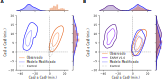
\includegraphics[width=0.9\textwidth]{img/cap_4/histogramas_extrinseco.png}
    \caption{\footnotesize{Gráficos de KDE con las predicciones de diferencia de tiempos entre máxima actividad de caspasas utilizando el modelo presentado por \cite{Albeck2008} modificado con la inclusión de los biosensores implementados y variando algunos parámetros. Se graficaron las curvas de nivel del KDE que encierran el 34\% y 68\% de los datos de diferencia de tiempos de máxima actividad observados experimentalmente (naranja) y el experimento control realizado con tres biosensores de caspasa 3 (gris). Adaptado de \cite{Corbat2018}. \textbf{A.} Se simuló cien veces el modelo variando la concentración inicial de los biosensores y fijando la concentración de ligando y receptor en $10^3$ (azul). \textbf{B.} Se simuló cien veces el modelo EARM 1.0 variando la concentración inicial de los biosensores (violeta) y luego se repitieron las simulaciones fijando la concentración inicial de ligando y receptor en $10^3$ y XIAP en $10^2$ (azul).}}
    \label{fig:hist_extrinseco}
\end{figure}

\begin{figure}[t!]
    \centering
    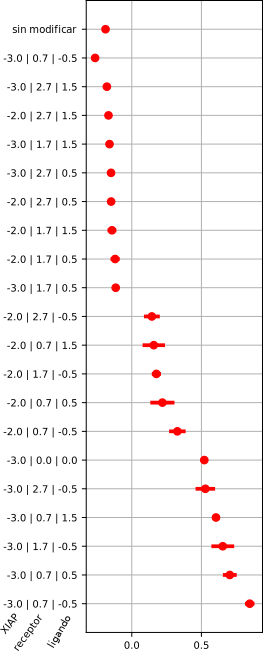
\includegraphics[width=0.4\textwidth]{img/cap_4/supplementary_4_A.pdf}
    \caption{\footnotesize{Se simuló el modelo EARM 1.0 modificado variando la concentración inicial del ligando, receptor y XIAP, multiplicándolos por 10 elevado al valor presentado. Se armaron histogramas bidimensionales con una cuadrícula de 4 a 6 minutos y se calculó la superposición con el histograma obtenido experimentalmente. Se vio que reducir la concentración de XIAP a $10^2$, el ligando a $10^3$ y aumentar la concentración del receptor a $10^3$ era la mejor combinación. Adaptado de \cite{Corbat2018}.}}
    \label{fig:cuad_min}
\end{figure}

A continuación, se buscó una especie que regule la diferencia entre tiempos de máxima actividad de la caspasa intrínseca y efectora sin afectar los otros resultados. Se vio que la proteína inhibidora de apoptosis ligada al cromosoma X (XIAP) inhibe a la caspasa efectora y a su vez es inhibida por Smac una vez liberada por la mitocondria post permeabilización de membrana. Reducir la concentración de XIAP a $10^2$ invierte el orden predicho entre la caspasa intrínseca y efectora, llegando a una descripción correcta de los tiempos entre caspasas (ver \cref{fig:hist_extrinseco}B). Para seleccionar los valores de las condiciones iniciales que mejor describan los resultados de tiempos experimentales, se construyeron los histogramas bidimensionales de diferencias de tiempo de máxima actividad para cada conjunto de parámetros y se calculó la superposición entre ambos (ver \cref{fig:cuad_min}).

Se verificó que el modelo modificado todavía predice los resultados presentados en el trabajo de \cite{Albeck2008}. Se corroboró que los anchos de las curvas de actividad sigan dentro de lo predicho previamente. Además se mantuvo el desencadenamiento abrupto posterior a la permeabilización de membrana, y se pudo apreciar el origen de la predicción realizada previamente donde la mayor parte de la caspasa extrínseca es activada debido a una retroalimentación. Este hecho acompaña nuestras observaciones experimentales donde la caspasa efectora alcanza el máximo de actividad antes que la extrínseca.


%%%%%%%%%%%%%%%%%%%%%%%%%%%%%%%%%
\section{Desarrollo de \textit{Apoptotic Reaction Model}}


Habiendo modificado el modelo para describir correctamente la diferencia entre tiempos de máxima actividad de caspasas al utilizar estímulos extrínsecos, se procedió a adaptarlo para predecir resultados en experimentos con estímulos intrínsecos. Dado que el modelo modificado contiene el módulo intrínseco, nos basamos en el trabajo de \cite{Zhang2009} para agregar una especie que simbolice el estímulo intrínseco. Dicha especie trunca a Bid, de la misma forma como lo hace la caspasa extrínseca. Se probaron distintos nodos para iniciar el estímulo, obteniendo resultados idénticos en todos los casos debido al desencadenamiento abrupto de la cascada post permeabilización de membrana mitocondrial.

Nuevamente, se simuló el sistema variando la concentración de los tres biosensores simultáneamente. A partir del estado del ensamble de biosensores se calcularon las correspondientes curvas de anisotropía, para luego analizarlas con el mismo protocolo que se usó en los experimentos. El modelo predecía que la caspasa intrínseca sería la primera en alcanzar la máxima actividad, seguida aproximadamente 30 minutos después por la efectora y otros 30 minutos después por la extrínseca (ver \cref{fig:exp_vs_Corbat}).

\begin{figure}[b!]
    \centering
    \includegraphics[width=0.9\textwidth]{img/cap_4/exp_vs_Corbat.png}
    \caption{\footnotesize{Gráficos de KDE con las predicciones de diferencia de tiempos entre máxima actividad de caspasas utilizando el modelo presentado en \cite{Corbat2018} modificado con la inclusión de estímulo intrínseco. Se simuló cien veces el modelo con cada estímulo variando la concentración inicial de los biosensores.  Adaptado de \cite{Corbat2021}. \textbf{A.} Se graficó la región que contiene a todas las curvas de anisotropía y actividad simuladas y se remarcó la curva cuya concentración corresponde a la mediana de concentraciones. En el modelado se usaron sCas3-BP, sCas8-RP y sCas9-GP. \textbf{B.} Se graficaron las curvas de nivel del KDE que encierran el 68\% de los datos de diferencia de tiempos de máxima actividad observados experimentalmente (celeste para extrínseco y naranja  para intrínseco) y el 34\% de las cien simulaciones (violeta para extrínseco y rojo  para intrínseco). Aunque la dinámica esta bien descripta por el modelo al usar estímulos extrínsecos, el orden de las caspasas efectora e intrínseca se encuentran invertidos al simularlo con estímulos intrínsecos.}}
    \label{fig:exp_vs_Corbat}
\end{figure}

En primer lugar, se barrieron las concentraciones iniciales de la caspasa 6, caspasa intrínseca, Apaf y citocromo C, así como las constantes cinéticas de activación de Apaf por el citocromo C, la conversión de Apaf en el apoptosoma, la inhibición de XIAP por Smac, la unión entre caspasa 6 y la caspasa extrínseca y las constantes de unión entre las caspasas y los tres biosensores. Todos estos parámetros fueron estudiados ya que controlan especies que se encuentran en la rama que conecta la caspasa intrínseca y la efectora. Aunque no se halló ninguna combinación de parámetros que genere un modelo capaz de describir experimentos con estímulo intrínseco y extrínseco al mismo tiempo, si fue posible trasladar las diferencias de tiempos para describir los experimentos con estímulo intrínseco, sacrificando los resultados previos (ver \cref{fig:CorbatForzado}). En este caso, el biosensor de caspasa intrínseca no llega a clivarse en su totalidad en el transcurso de las 15 horas simuladas.

\begin{figure}
    \centering
    \includegraphics[width=0.9\textwidth]{img/cap_4/force_corbat.png}
    \caption{\footnotesize{Gráficos de las predicciones utilizando el modelo presentado en \cite{Corbat2018} modificado con la inclusión de estímulo intrínseco y para que la diferencia de tiempos de máxima actividad de caspasas al utilizar estímulos intrínsecos esté bien descripta. Se simuló cien veces el modelo con cada estímulo variando la concentración inicial de los biosensores.  Adaptado de \cite{Corbat2021}. \textbf{A.} Se graficó la región que contiene a todas las curvas de anisotropía y actividad simuladas y se remarcó la curva cuya concentración corresponde a la mediana de concentraciones. En el modelado se usaron sCas3-BP, sCas8-RP y sCas9-GP. \textbf{B.} Se graficaron las curvas de nivel del KDE que encierran el 68\% de los datos de diferencia de tiempos de máxima actividad observados experimentalmente (celeste para extrínseco y naranja  para intrínseco) y el 34\% de las cien simulaciones (violeta para extrínseco y rojo  para intrínseco). Aunque la dinámica esta bien descripta por el modelo al usar estímulos intrínsecos, la diferencia de tiempos de máxima actividad de caspasas para estímulos extrínsecos esta muy alejada de lo esperado y en ambos casos el biosensor de caspasa intrínseca no llega a clivarse en su totalidad.}}
    \label{fig:CorbatForzado}
\end{figure}


%%%%%%%%%%%%%%%%%%%%%%%%%%%%
\subsection{Evaluación de Modelos Previos}


Dado que no se hallaron combinaciones de parámetros que sean capaces de describir experimentos con ambos estímulos, se consideró realizar un barrido de parámetros utilizando varios modelos previamente publicados. \cite{Lopez2013} desarrollaron un paquete de Python denominado PySB (por las siglas de \ening{Python Systems Biology}) que permite definir modelos numéricos de diversos tipos y simularlos. Por medio de este paquete, es posible definir módulos que se pueden integrar para formar un modelo completo.  Dentro de dicho paquete, hay una librería de modelos, entre los que se encuentran muchas variantes del modelo de Apoptosis. Se definió un pequeño módulo que agregaba los biosensores desarrollados al modelo en estudio. Se realizó un barrido grueso de los mismos parámetros en los modelos desarrollados por \cite{Howells2011, Albeck2008, Cui2008, Chen2007} y \cite{Chen2007a}. El modelo cuyas predicciones de tiempo de máxima actividad entre caspasas más se acercaba a los valores obtenidos experimentalmente fue el denominado Albeck11f, publicado por \cite{Albeck2008} (ver \cref{fig:albeck11f}). Aunque estas diferencias estaban descriptas adecuadamente, la forma funcional de los perfiles de actividad eran notoriamente distintos. En particular, el biosensor de la caspasa intrínseca no llegaba a clivarse por completo en las 15~hr simuladas.

\begin{figure}
    \centering
    \includegraphics[width=0.9\textwidth]{img/cap_4/albeck11f.png}
    \caption{\footnotesize{Gráficos de las predicciones utilizando el modelo presentado en \cite{Albeck2008}, llamado 11F, modificado con la inclusión de estímulo intrínseco y para que la diferencia de tiempos de máxima actividad de caspasas al utilizar ambos estímulos esté lo mejor descripta posible. Se simuló cien veces el modelo con cada estímulo variando la concentración inicial de los biosensores.  Adaptado de \cite{Corbat2021}. \textbf{A.} Se graficó la región que contiene a todas las curvas de anisotropía y actividad simuladas y se remarcó la curva cuya concentración corresponde a la mediana de concentraciones. En el modelado se usaron sCas3-BP, sCas8-RP y sCas9-GP. \textbf{B.} Se graficaron las curvas de nivel del KDE que encierran el 68\% de los datos de diferencia de tiempos de máxima actividad observados experimentalmente (celeste para extrínseco y naranja  para intrínseco) y el 34\% de las cien simulaciones (violeta para extrínseco y rojo  para intrínseco). Aunque las diferencias de tiempos están relativamente bien descriptas por el modelo al usar ambos estímulos, los perfiles de actividad se alejan de lo observado experimentalmente y en ambos casos el biosensor de caspasa intrínseca no llega a clivarse en su totalidad.}}
    \label{fig:albeck11f}
\end{figure}


%%%%%%%%%%%%%%%%%%%%%%%%%%%%%%%%%%%%
\subsection{Retroalimentación entre Caspasa Efectora e Intrínseca}
\label{sec:modelo:feedback}


Al analizar el orden de máxima actividad de las caspasas utilizando estímulos extrínsecos, notamos que la caspasa efectora era la primera en llegar al máximo de actividad y que ésta, a través de su retroalimentación mediante la caspasa 6, activaba lo remanente de la caspasa extrínseca, llegando así al máximo de actividad. De forma análoga, al utilizar estímulos intrínsecos, la caspasa efectora también alcanza su máximo de actividad en primer lugar y la sigue la caspasa intrínseca. A diferencia de la vía extrínseca, no se describe ninguna retroalimentación entre las caspasas efectora e intrínseca en el modelo. Sin embargo, al revisar la bibliografía, encontramos que diversos modelos preparados para describir experimentos con estímulos intrínsecos, incluyen una retroalimentación entre la caspasa efectora y la intrínseca \citep{Zhang2009, Rehm2006}. Adicionalmente, \cite{McComb2019} hacen especial hincapié en su trabajo en la importancia que tiene dicha retroalimentación. Desde el punto de vista molecular, el apoptosoma se encuentra preformado por Apaf-1, procaspasa 9 y dATP/ATP. El mismo es subsecuentemente activado al unírsele citocromo C, liberado post permeabilización de membrana mitocondrial y generando una variante denominada caspasa 9 (p35/p12), capaz de activar a la caspasa efectora. Ésta, a su vez, retroalimenta a la caspasa 9 y forma la subespecie p35/p10 que tiene mayor actividad enzimática y no es inhibida por XIAP.

Se reemplazó la conversión de un solo paso del apoptosoma por las reacciones descriptas previamente. Se utilizó la especie Apaf para representar al apoptosoma inactivo, y esta especie cambia a su estado activo luego de interactuar con el citocromo C citoplasmático. A continuación Apaf activo puede clivar a la caspasa 3 (representando a la efectora), así como al biosensor, con una constante de reacción baja. Finalmente, la caspasa 3 cliva a Apaf activo generando la especie Apop (que representa la caspasa 9 p35/p12), que tiene constantes catalíticas con sus sustratos mayores a Apaf activo y, además, no interactúa con XIAP (ver \cref{fig:sketch_2021}). Utilizando parámetros iguales a los anteriores, eligiendo la constante cinética de Apaf activo 10 veces menor que la de Apop, el modelo predice un orden de máxima actividad de caspasas acorde a lo observado experimentalmente.

\begin{figure}
    \centering
    \includegraphics[width=0.5\textwidth]{img/cap_4/model_simplified.pdf}
    \caption{\footnotesize{Esquema simplificado del modelo de red de caspasas modelado. Se pueden apreciar las ramas que intercomunican cada módulo. En particular, el módulo extrínseco activa el intrínseco y efector. El módulo intrínseco también activa el módulo efector. Y el módulo efector tiene una retroalimentación sobre el módulo extrínseco e intrínseco. Adaptado de \cite{Corbat2021}.}}
    \label{fig:sketch_2021}
\end{figure}

Se utilizó el paquete de Python lmfit \citep{newville_2014} para hallar la mejor combinación de parámetros del modelo que describa los resultados obtenidos experimentalmente. Se utilizaron una búsqueda por cuadrilla (un método de fuerza bruta donde se varían las distintas combinaciones de todos los parámetros de forma equiespaciada) y luego \ening{Adaptive Memory Programming for Global Optimization} (AMPGO) \citep{Lasdon2010}. Los parámetros barridos fueron: las constantes de unión de todos los biosensores, Apaf activo al biosensor intrínseco y caspasa 3 a Apaf; así como las concentraciones iniciales de los biosensores, Apaf, XIAP y citocromo C. Los algoritmos utilizados buscaban minimizar las diferencias entre las predicciones de diferencias de tiempos de máxima actividad observadas y simuladas, y también, que el ancho de actividad de las caspasas sea el esperado. Los objetivos eran obtener 10 minutos de diferencia entre caspasa 9 y 3 y 5.5 minutos entre caspasa 8 y 3, al usar estímulo extrínseco; y 4 minutos entre caspasa 9 y 3 y 9 minutos entre caspasa 8 y 3 al utilizar estímulo intrínseco. Con todos los estímulos, se buscó un ancho de actividad de 15 minutos para la caspasa 3 y 8, y de 30 minutos para la caspasa 9. Una vez que ambos algoritmos hallaron la mejor combinación de parámetros, se hizo una mejora manual más fina de ellos. Éste modelo se llamó \textit{Apoptotic Reaction Model} (ARM, ya que surgió de \textit{Extrinsic Apoptotic Reaction Model} pero no es solo para estímulos extrínsecos) y se encuentra publicado en \cite{Corbat2021} y subido a \href{https://github.com/acorbat/caspase_model/tree/master}{caspase\textunderscore model} y \href{https://www.ebi.ac.uk/biomodels/MODEL2105210001}{Biomodels}  (ver apéndice \ref{repositorio}, \cite{Malik-Sheriff2018}).

Habiendo hallado la mejor combinación de parámetros, se simuló el modelo 100 veces variando la concentración inicial de los biosensores de forma correlacionada. Los tiempos obtenidos a partir del análisis de las curvas de anisotropía simuladas muestran un buen correlato con lo observado experimentalmente, así como los perfiles de actividad generados. En particular, se puede apreciar que la caspasa intrínseca tiene un perfil hiperbólico mientras que la efectora y extrínseca tienen un perfil sigmoideo (ver \cref{fig:ARM}). Cabe destacar que la concentración de las especies relacionadas a la caspasa intrínseca tienen un orden de magnitud menor que las propuestas previamente y, por lo tanto, se asemejan a estimaciones experimentales de su concentración.

\begin{figure}
    \centering
    \includegraphics[width=0.9\textwidth]{img/cap_4/arm.png}
    \caption{\footnotesize{Gráficos de las predicciones utilizando \textit{Apoptotic Reaction Model} \citep{Corbat2021}. Se simuló cien veces el modelo con cada estímulo variando la concentración inicial de los biosensores.  Adaptado de \cite{Corbat2021}. \textbf{A.} Se graficó la región que contiene a todas las curvas de anisotropía y actividad simuladas y se remarcó la curva cuya concentración corresponde a la mediana de concentraciones. En el modelado se usaron sCas3-BP, sCas8-RP y sCas9-GP. Al igual que en los experimentos (ver \cref{fig:curvas_experimentales}), la caspasa intrínseca tiene un perfil hiperbólico mientras que la efectora y extrínseca tienen un perfil sigmoideo. \textbf{B.} Se graficaron las curvas de nivel del KDE que encierran el 68\% de los datos de diferencia de tiempos de máxima actividad observados experimentalmente (celeste para extrínseco y naranja  para intrínseco) y el 34\% de las cien simulaciones (violeta para extrínseco y rojo  para intrínseco). La diferencia de tiempos de máxima actividad de caspasas para ambos estímulos se encuentra en concordancia con lo observado experimentalmente.}}
    \label{fig:ARM}
\end{figure}


%%%%%%%%%%%%%%%%%%%%%%%%%%%%%%%%
\section{Análisis de la Capacidad Predictiva}


A continuación, se evaluó la capacidad de ARM de describir resultados observados previamente sobre el comportamiento de la red apoptótica. En particular, se analizó el comportamiento de la red ante variaciones en la intensidad del estímulo utilizado \citep{Zhang2009, Albeck2008}, las susceptibilidades de la red ante variaciones en la concentración inicial de algunas especies \citep{Gaudet2012, Spencer2009, Rehm2006}, y la propagación de la señal ante ausencias de algunas caspasas específicas \citep{McComb2019, Inoue2009}.


%%%%%%%%%%%%%%%%%%%%%%%%%%%%
\subsection{Intensidad del estímulo}


El momento en que se desencadena la cascada apoptótica es, en promedio, inversamente proporcional a la intensidad del estímulo utilizado, tanto intrínseco como extrínseco \citep{Zhang2009, Albeck2008}. Para analizar este comportamiento, se simuló el modelo variando la intensidad de los estímulos a lo largo de 3 ordenes de magnitud. En ambos casos se pudo apreciar el comportamiento esperado (ver \cref{fig:BarridoEstimulo}A). Es interesante notar que las diferencias de tiempo de máxima actividad entre caspasas prácticamente no se ven afectadas por la intensidad del estímulo (ver \cref{fig:BarridoEstimulo}B). Aunque se puede ver que para estímulos extrínsecos hay un pequeño corrimiento, éste es del orden de unos pocos minutos y sería difícil de apreciar experimentalmente.

\begin{figure}
    \centering
    \includegraphics[width=0.7\textwidth]{img/cap_4/barrido_estimulo.pdf}
    \caption{\footnotesize{Se analizaron los efectos de variar la intensidad de los estímulos sobre los tiempos de máxima actividad de las caspasas en ARM.  Adaptado de \cite{Corbat2021}. \textbf{A.} Se graficaron los tiempos de máxima actividad de la caspasa efectora en función de la intensidad del estímulo utilizado. La dependencia entre el desencadenamiento de la apoptosis y la intensidad del estímulo es inversamente proporcional con ambos tipos de estímulos. \textbf{B.} Se graficaron la diferencia de tiempos de máxima actividad entre caspasas al utilizar ambos tipos de estímulos (naranja intrínseco y celeste extrínseco) a lo largo de tres ordenes de magnitud. Debido al desencadenamiento rápido de la cascada, la intensidad del estímulo intrínseco no varía la diferencia de tiempo de máxima actividad entre caspasas. Por otro lado, variar la intensidad del estímulo extrínseco introduce un pequeño cambio en las diferencias de tiempo de máxima actividad que sería difícil de distinguir experimentalmente.}}
    \label{fig:BarridoEstimulo}
\end{figure}

\begin{figure}[t!]
    \centering
    \includegraphics[width=0.5\textwidth]{img/cap_4/sweep_int_stim.png}
    \caption{\footnotesize{Gráficos que muestran la concentración en función del tiempo de especies mitocondriales ante estímulos intrínsecos de distintos ordenes de magnitud. En particular se graficaron los estados de multimerización de Bax activo, Mito activo que representa los poros en la membrana mitocondrial y la concentración de citocromo C citoplasmático, que es el resultado final de la permeabilización de la membrana mitocondrial. Es de notar que al formarse unos pocos poros en la membrana, la liberación de citocromo C ocurre rápidamente y de ahí el desencadenamiento rápido de la cascada apoptótica. Adaptado de \cite{Corbat2021}.}}
    \label{fig:desencadenamiento_rapido}
\end{figure}

Se corroboró además que se mantiene el comportamiento de desencadenamiento abrupto de la cascada una vez alcanzada la permeabilización de membrana mitocondrial. Esto se aprecia fácilmente al ver que utilizando distintos ordenes de intensidad de estímulo intrínseco, las especies contenidas dentro de la mitocondria se liberan rápidamente una vez que se forman unos pocos (1 a 3) poros en la membrana (ver \cref{fig:desencadenamiento_rapido}). Este comportamiento se vio experimentalmente y se describió en \cite{Albeck2008}.


%%%%%%%%%%%%%%%%%%%%%%%
\subsection{Sensibilidad de los Observables}


Se realizó un análisis de sensibilidad de los observables a las concentraciones iniciales (no nulas) de las distintas especies. Esto trae aparejado dos beneficios: por un lado brinda un mejor entendimiento de la red y cómo los distintos parámetros afectan a los observables; y además, permite simular el efecto sobre los observables de experimentos análogos a reducir o incrementar la concentración de alguna especie en particular. Para dicho análisis, se incrementó y disminuyó la concentración de cada condición inicial por separado en medio orden de magnitud y un orden de magnitud y se estimaron los siguientes observables: inicio de la cascada (tiempo del máximo de actividad de la caspasa efectora), diferencia entre tiempos de máxima actividad de las caspasas iniciadoras y la efectora, y el ancho del perfil de actividad de cada caspasa (definido como el ancho de la mitad del máximo de actividad). Para calcular la sensibilidad se utilizó

\begin{equation*}
S = \frac{dObs}{d log k} = \frac{Obs_{per} - Obs}{log 10^{f} k - log k} = \frac{Obs_{per} - Obs}{f}.
\end{equation*}

\noindent Dado que cada concentración inicial k se incrementó y redujo en un orden y medio orden de magnitud, el denominador solo tomará los valores de $\pm 1$ y $\pm -1/2$. Al no haber grandes diferencias entre variar uno o medio orden de magnitud, nos concentraremos en describir el caso donde se incrementó medio orden de magnitud cada concentración inicial.

\begin{figure}[t!]
    \centering
    \includegraphics[width=0.7\textwidth]{img/cap_4/sensitivity_05.pdf}
    \caption{\footnotesize{Estudio de sensibilidad de los observables ante incrementar (\textbf{A}) y reducir (\textbf{B}) medio orden de magnitud cada concentración inicial del modelo. Los colores de cada elemento resaltan si hubo una diferencia apreciable en el observable. Las especies escritas en rojo con reborde negro corresponden a inhibidores. Adaptado de \cite{Corbat2021}.}}
    \label{fig:sensitividad05}
\end{figure}

\begin{figure}[t!]
    \centering
    \includegraphics[width=0.7\textwidth]{img/cap_4/sensitivity_10.pdf}
    \caption{\footnotesize{Estudio de sensibilidad de los observables ante incrementar (\textbf{A.}) y reducir (\textbf{B.}) un orden de magnitud cada concentración inicial del modelo. Los colores de cada elemento resaltan si hubo una diferencia apreciable en el observable. Las especies escritas en rojo con reborde negro corresponden a inhibidores. Adaptado de \cite{Corbat2021}.}}
    \label{fig:sensitividad10}
\end{figure}

En el trabajo de \cite{Gaudet2012} se discuten en profundidad los efectos de variar las concentraciones iniciales de diversas especies sobre el momento en el que se desencadena la apoptosis al utilizar estímulos extrínsecos. Esto puede resumirse en como la sobreexpresión de inhibidores (FLIP, BAR, Bcl2 y XIAP) retrasan el inicio, mientras que caspasas, receptores y miembros proapotóticos de la familia BH3 la aceleran. Es de interés notar que Smac, citocromo C y Apaf no tienen ningún efecto. Estas predicciones están en acuerdo con experimentos realizados por \cite{Gaudet2012} para Bcl-2 y Bid y por \cite{Spencer2009} para FLIP y Bid. Análogamente, hay muchas similitudes con el análisis de sensibilidad al utilizar estímulos intrínsecos. Perturbaciones experimentales de Smac, XIAP y procaspasa 3 y 7 fueron realizadas por \cite{Rehm2006} y también acompañan lo descripto por el modelo. En particular, aumentar XIAP retrasa el inicio, las procaspasas 3 y 7 lo adelantan, mientras que Smac no tiene ningún efecto.

Al utilizar estímulos extrínsecos, la concentración inicial de Apaf y el biosensor de la caspasa intrínseca tienen un efecto sobre la diferencia de tiempos entre la caspasa efectora e intrínseca. El tiempo entre el máximo de actividad de la caspasa efectora y extrínseco se reduce levemente al aumentar Bcl-2 y la caspasa 6. En cuanto a las diferencias de tiempo de máxima actividad de caspasas al utilizar estímulos intrínsecos, Apaf afecta principalmente el tiempo entre caspasa efectora e intrínseca. De forma similar, el tiempo entre caspasa efectora y extrínseca se ve reducido por las especies involucradas en su retroalimentación como la caspasa 6 o la caspasa extrínseca. En contraposición, aumentar la concentración de la caspasa efectora, acelera su activación por retroalimentación y la adelanta respecto a la extrínseca, o también, aumentar los inhibidores de la caspasa extrínseca como BAR.

Estos resultados tienen valor tanto experimental ya que resumen qué concentraciones pueden afectar a cuáles observables, así como valor descriptivo del modelo ya que nos brindan información de qué parámetros no pueden ser precisamente determinados con los observables utilizados. Por otro lado, si uno necesitase modificar el modelo para incluir más experimentos, estas tablas dan cuenta de qué parámetros pueden modificarse sin afectar predicciones previas.


%%%%%%%%%%%%%%%%%%%%%%%%%%
\subsection{Propagación de la señal}

Por último, se simularon experimentos de 24~hr con ambos tipos de estímulos, llevando a cero la concentración de alguna o algunas caspasas para emular experimentos de \ening{Knock-Out} (KO). En los trabajos de \cite{Inoue2009} y \cite{McComb2019}, se knockean las caspasas 3, 6, 7, 8 y 9 o un subconjunto de ellas, para luego estimular las células de forma extrínseca o intrínseca. Luego de varias horas, se procede a lisarlas y estudiar la presencia de las distintas caspasas activas o inactivas mediante Western Blot. Aunque estos experimentos se realizaron en líneas celulares distintas a las que utilizamos previamente, esperamos que el comportamiento de la cascada sea similar. La propagación de la señal y las caspasas activas en cada situación descriptas por el modelo fueron las esperadas en acuerdo con lo observado experimentalmente (ver \cref{fig:KOCaspasas}).

\begin{figure}
    \centering
    \includegraphics[width=0.7\textwidth]{img/cap_4/ko_table.pdf}
    \caption{\footnotesize{Se simularon experimentos en los que las concentraciones iniciales de un subconjunto de procaspasas se llevaba a cero para simular su KO. Se marcó con ticks cada caspasa que se halló activa en la simulación de 24~hr, mientras que se puso una cruz cuando su actividad fue nula o despreciable. En todos estos experimentos se obtuvo una predicción que se condice con el resultado experimental. Adaptado de \cite{Corbat2021}.}}
    \label{fig:KOCaspasas}
\end{figure}

Para empezar, dado que las caspasas 3 y 7 reconocen el mismo sitio de unión y son efectoras, los experimentos KO de alguna de ellas se simularon restando la mitad de la concentración inicial de caspasa efectora. Esto llevó a que simular KO de caspasa 3 ó 7 den resultados idénticos, donde se reduce la actividad de estas caspasas, pero se obtiene una respuesta completa de todas las caspasas en el largo plazo. Si se KO la caspasa 6 y se utiliza un estímulo extrínseco, se reduce levemente la dinámica de las caspasas, pero tampoco se aprecia una diferencia en el largo plazo. Contrariamente, si se utiliza un estímulo intrínseco, la caspasa extrínseca nunca llega a activarse. No nos debe sorprender que KO de la caspasa de la vía correspondiente al estímulo que se usa, resulta en que no haya actividad apreciable de ninguna caspasa (ver \cref{fig:KO_singles}).

\begin{figure}[b!]
    \centering
    \includegraphics[width=0.75\textwidth]{img/cap_4/ko_singles.pdf}
    \caption{\footnotesize{Se simuló la cascada apoptótica llevando a cero la concentración de las procaspasas 3 (\textbf{A}), 6 (\textbf{B}), 8 (\textbf{C}) y 9 (\textbf{D}). Adaptado de \cite{Corbat2021}. \textbf{A.} Al hacer un KO de la caspasa 3, solo se ve una dinámica levemente más lenta que no será apreciable en experimentos de larga duración ya que ésta caspasa es redundante con la caspasa 7. \textbf{B.} Un KO de la caspasa 6 interrumpirá cualquier señal que pase de la caspasa efectora a la extrínseca. Es así que al usar estímulos extrínsecos, solo se ve una dinámica más lenta en la caspasa 8 por falta de retroalimentación, mientras que si se usan estímulos intrínsecos, la caspasa 8 nunca se activa. \textbf{C} y \textbf{D.} Al hacer KO de las caspasas iniciadoras, se bloquea todo actividad de caspasas al usar el estímulo correspondiente. Si se usa el estímulo opuesto al de la caspasa KO, entonces se observa actividad prácticamente normal.}}
    \label{fig:KO_singles}
\end{figure}

Doble KO de alguna caspasa efectora (3 ó 7) y la caspasa 6 llevó a células con una dinámica más lenta pero que culminaban en muerte celular. De forma similar a las células con KO de caspasa 6, al utilizar estímulos intrínsecos en estos casos, la caspasa extrínseca no llega a activarse. Aplicar un KO de ambas caspasas efectoras 3 y 7, con o sin caspasa 6 incluida, llevan a que no haya ninguna actividad de caspasa efectora. Utilizar estímulos extrínsecos llevan a que haya actividad de la caspasa extrínseca, pero la actividad de la caspasa intrínseca es despreciable. Además, si se utiliza un estímulo intrínseco en estos casos, no se puede apreciar actividad de ninguna caspasa, excepto la versión lenta de la caspasa intrínseca no completamente activa (descripta por \cite{Rehm2006} y en la sección \ref{sec:modelo:feedback}). En los experimentos esta actividad no se aprecia, probablemente debido a la degradación de especies que no fue incluida en el modelo. Cabe destacar que este comportamiento no puede ser descripto por los modelos previos ya que en todos ellos la retroalimentación a la caspasa intrínseca está ausente y ésta siempre se activaría por completo (ver \cref{fig:KO_dobles}).

\begin{figure}[b!]
    \centering
    \includegraphics[width=0.75\textwidth]{img/cap_4/ko_multis.pdf}
    \caption{\footnotesize{Se simuló la cascada apoptótica llevando a cero la concentración de los subconjuntos de las procaspasas 3 y 7  (\textbf{A}); 3 y 6 (\textbf{B}); y 3, 6 y 7 (\textbf{C}). Adaptado de \cite{Corbat2021}. \textbf{A.} En las células KO para todas las caspasas efectoras, solo se aprecia actividad de la caspasa 9 (p35/p12) y de la caspasa 8 si el estímulo es extrínseco. \textbf{B.} Células sin caspasa 3 y 6, muestran una baja actividad de la caspasa efectora y una dinámica más lenta de la caspasa 8 (si son extrínsecamente estimuladas), pero normal en tiempos largos. \textbf{C} Si se KO las caspasas 3, 6 y 7, sólo se ve una actividad muy baja por parte de la caspasa 9 (p35/p12) que no podría ser apreciada experimentalmente y, si las células son estimuladas extrínsecamente, algo de actividad de la caspasa 8 también.}}
    \label{fig:KO_dobles}
\end{figure}

La adición de la retroalimentación entre las caspasas efectoras e intrínsecas sirvió tanto para recuperar la dinámica entre tiempos de máxima actividad entre caspasas como para incluir el comportamiento de la red ante experimentos de KO de caspasas. Cabe destacar que la variante p35/p12 de la caspasa intrínseca, al ser considerablemente más lenta que la variante p35/p10, permite reproducir resultados en los que las caspasas efectoras están knockeadas. Con los modelos previos, la única variante de la caspasa intrínseca se activa por completo una vez permeabilizada la membrana mitocondrial, mientras que en ARM solo se aprecia una baja actividad por parte de la variante p35/p12.


%%%%%%%%%  Conclusión
\chapter{Conclusiones y Discusiones}

En el presente trabajo, se generó el primer modelo integrador de la cascada apoptótica, que hemos denominado \textit{Apoptotic Reaction Model}, capaz de reproducir la dinámica de sus módulos ante estímulos categóricamente distintos, así como resultados publicados previamente por otros grupos. Para ello, fue necesario desarrollar y caracterizar un arreglo de biosensores que permita observar la actividad de cada módulo de la red de caspasas a nivel de célula única. Con ellos se obtuvo un cuerpo de datos cohesivo que surgió de interrogar la dinámica de cada módulo ante estímulos intrínsecos y extrínsecos. Luego de encontrar discrepancias entre las predicciones de los modelos utilizados y las observaciones experimentales, se identificó una retroalimentación ausente en los modelos, cuyas reacciones debieron ser añadidas para generar un modelo completo. Adicionalmente, se simularon experimentos descriptos en trabajos previos para corroborar que el modelo generado conserva la capacidad predictiva de otros experimentos.

El procedimiento aplicado aquí para estudiar la red de caspasas puede ser extrapolado a otras redes biológicas. A grandes rasgos, éste consistió en diseñar un biosensor y su correspondiente análisis para obtener un observable robusto que sirva para describir la dinámica de los módulos que componen a la red. Luego, la red deberá ser interrogada y perturbada de formas distintas para generar un cuerpo de datos que describa su comportamiento en cada situación. Finalmente, estudiar e integrar diversos modelos que describan cada módulo o la totalidad de la red y corroborar que las modificaciones introducidas describen las nuevas observaciones, así como los experimentos previos.

En el \cref{cap:MatMet}, se planteó un experimento en el que se deseaba estudiar la actividad de una proteasa a partir de un biosensor basado en homoFRET. Combinando modelado y ley de acción de masas con el entendimiento del origen de la señal fotofísica a partir del estado del ensamble de biosensores, se demostró un método para reportar la actividad enzimática a cada tiempo.  Utilizar las curvas de actividad en lugar de la señal del reportero sin procesar trae la ventaja, no solo de su valor biológico, sino que también es posible compararlas con resultados de simulaciones del sistema.

Estimar un observable de índole biológica es importante para comprender el comportamiento de la red, pero a esto hay que agregarle una forma de lidiar con la elevada variabilidad que tienen estos sistemas. Aquí se combinaron dos metodologías que permiten sortear dicho problema: utilizar técnicas de alto rendimiento y un observable robusto. En primer lugar, se buscó automatizar la adquisición y análisis de imágenes para así generar un cuerpo de datos con el que se pueda describir la población de células. Se realizó un estudio detallado de distintos algoritmos que podían ser utilizados, así como posibles sesgos que estos introducían, para generar un flujo de análisis automatizado. En segundo lugar, se comprobó que la diferencia de tiempos de máxima actividad de caspasas esta mucho mejor conservado que utilizar uno sólo de ellos ya que el momento en que se desencadena la apoptosis es mucho más variable que el tiempo que transcurre entre el máximo de actividad de cada caspasa. Se debe destacar también que combinar técnicas de alto rendimiento con un análisis de reducción de datos permite generar cuerpos de datos fácilmente interpretables.

Habiendo discutido la metodología por la cual se interrogaría la red de caspasas de forma automática y cuál es el observable a obtener, se introdujo en el \cref{cap:Biosensores} una caracterización de los biosensores a implementarse. El análisis inicial de las combinaciones de fluoróforos realizado en el Instituto Max Planck de Fisiología Molecular sirvió de base para implementar los sensores basados en homoFRET que se utilizaron en los distintos experimentos. Con el objetivo de traducir las curvas de anisotropía en la actividad correspondiente a cada caspasa, se procedió a caracterizar distintos parámetros de los pares de fluoróforos. Por un lado, se determinó el valor de $b$, la relación entre los brillos de los biosensores en estado dimérico y monomérico, a través de un experimento en el que se generaron tres biosensores de colores distintos pero sensibles a la misma caspasa. Por otro lado, las anisotropías del dímero y monómero se determinaron para cada curva particular debido al efecto que tienen sobre estos valores los errores en la estimación de la intensidad.

Se buscó disminuir la variabilidad en la estequiometría de los biosensores añadidos de forma exógena, que a su vez aumentaba la varianza de los observables biológicos por efecto de secuestro que los biosensores tienen sobre las caspasas, implementando la construcción de un único plásmido que codifique para los tres biosensores separados por secuencias virales 2A. Mediante citometría de flujo y espectroscopia de correlación de fluorescencia se caracterizó la equimolaridad en la expresión de CASPAM, el plásmido desarrollado. Por último, se vio que el desvío estándar de las diferencias de tiempo de máxima actividad de las caspasas es menor en células transfectadas con CASPAM que con los tres sensores en plásmidos separados.

Una vez diseñada la metodología experimental por medio de la cual se interrogará la actividad de caspasas, se procedió a construir un cuerpo de datos que describa la dinámica de la red de caspasas ante estímulos intrínsecos y extrínsecos. Se apreció que la caspasa efectora es la primera en alcanzar el máximo de actividad sin importar el estímulo utilizado. Esto resulta de interés ya que si miramos el flujo de información, uno esperaría que las caspasas iniciadoras sean las primeras en alcanzar el máximo de actividad. Sin embargo, debido a que las caspasas iniciadoras se encuentran inhibidas para evitar que pequeños estímulos desencadenen la cascada, éstas alcanzan su máximo de actividad una vez que las caspasas efectoras las retroalimentan.

Finalmente, se construyó un modelo basado en ecuaciones diferenciales ordinarias y ley de acción de masas para describir la dinámica de la cascada apoptótica ante ambos tipos de estímulo. Como punto de partida, se utilizó un modelo preparado por \cite{Albeck2008} para describir el comportamiento de la red ante estímulos extrínsecos. Modificando las concentraciones iniciales del receptor, el ligando y XIAP fue posible recuperar la dinámica observada ante estímulos extrínsecos sin afectar predicciones previas. No obstante, no fue posible encontrar una combinación de parámetros, en este modelo y en otros similares publicados, que sirva para describir al mismo tiempo la dinámica con estímulos intrínsecos. La diferencia principal entre las predicciones de dichos modelos y lo que se observó experimentalmente, fue el orden de los máximos de actividad de la caspasa intrínseca y la efectora. De esta forma, se detectó que la retroalimentación de la caspasa efectora a la intrínseca estaba ausente en los modelos utilizados. Una vez añadida, se encontró un conjunto de parámetros que permitió describir la dinámica de la red de caspasas ante ambos tipos de estímulos simultáneamente.

Con el objetivo de corroborar que el modelo desarrollado conserva la capacidad predictiva, se simularon experimentos previos efectuados por otros grupos. En primer lugar, se simuló la red con intensidades crecientes de estímulo para ver que el tiempo en el que se desencadena la apoptosis, representado aquí por el tiempo de máxima actividad de la caspasa efectora, es inversamente proporcional a la intensidad del estímulo. En segundo lugar, se vio que el modelo conserva el desencadenamiento rápido de la cascada ya que ante la formación de pocos poros en la membrana mitocondrial, su contenido se libera rápidamente al citosol. Luego, se realizó un estudio de sensibilidad de observables ante cambios de la concentración inicial de todas las especies distintas de cero. Se pudo apreciar que muchas de las especies cuyo cambio afectaba el tiempo en el que se desencadenaba la cascada también había sido reportado en experimentos previamente. Por último, en forma análoga a experimentos donde se \textit{knockea} algún subconjunto de caspasas, se simularon casos en donde algunas caspasas estaban ausentes. Esto sirvió para estudiar el flujo de la señal en la red perturbada y se pudieron reproducir los resultados de los experimentos. Más importante, se pudieron reproducir resultados de experimentos donde se bloquean las caspasas efectoras que no se podrían reproducir con la topología de los modelos anteriores.

Unificar la información adquirida a través de los distintos experimentos en los que se pone a prueba la cascada apoptótica en un único modelo integrador es importante para generar predicciones confiables en terapias personalizadas, como en \cite{Eduati2020}. Como discutieron previamente \cite{Santolini2018}, determinar la topología de la red es crucial para descubrir los comportamientos emergentes del sistema bajo estudio. Modelos con un elevado nivel de detalle y que incluyen muchas especies podrían integrarse con otros modelos que describan otras vías, llevando en última instancia a uno de los desafíos propuestos por \cite{Karr2015}, un modelo de célula completa.

Con el objetivo de que tanto la metodología utilizada, así como los sensores desarrollados y los modelos diseñados puedan ser aplicados en distintos contextos y mejorados, todo fue publicado y subido en artículos científicos y repositorios. Los modelos desarrollados se encuentran disponibles para descargar en \href{https://github.com/acorbat/caspase_model/tree/master}{caspase\textunderscore model} y \href{https://www.ebi.ac.uk/biomodels/MODEL2105210001}{Biomodels} (MODEL2105210001, ver apéndice \ref{repositorio}). Tener fácil acceso a los modelos desarrollados permite probarlos en contextos distintos, y de ser necesario, completarlos. 

En esta tesis, se interrogó la dinámica de la cascada apoptótica ante ciertos estímulos extrínsecos e intrínsecos en células inmortalizadas de cáncer de cérvix generándose un modelo integrador que describe la dinámica de las caspasas y recapitula resultados de experimentos previos. Dentro de la amplia variedad de contextos biológicos donde apoptosis juega un papel importante, aquí nos hemos focalizado en estos dos estímulos para desarrollar una metodología integral de cuantificación y modelado de una red. La metodología desarrollada es una herramienta valiosa para analizar como se reconfigura la red en otras situaciones. Sería interesante introducir la síntesis y degradación de especies del modelo que no fueron tenidas en cuenta ya que en nuestro caso particular todos los experimentos se realizaron con cicloheximida por lo que la síntesis proteica estaba inhibida. Incluir síntesis y degradación de especies en el modelo será importante para predecir comportamientos ante estímulos oscilatorios o actividad subletal de caspasas, como durante la plasticidad neuronal \citep{Unsain2015}. Por otro lado, este modelo podría utilizarse para comparar la propagación de señales por la red en apoptosis tipo I (independiente de permeabilización mitocondrial) o tipo II (dependiente de permeabilización mitocondrial) en función de la concentración de XIAP y procaspasa \citep{Aldridge2014}. También resulta de interés analizar el papel de la cascada apoptótica en el control de la homeostasis de tejidos epiteliales, como fue analizado por \cite{Gagliardi2021}, \cite{Aoki2013} y \cite{Albeck2013}, así como su rol en la formación de patrones en el desarrollo epidermal de \textit{Drosophila Melanogaster} \citep{Crossman2018}. Estos son solo una pequeña selección de los diversos contextos en los que se podría estudiar la cascada en búsqueda de una descripción aún más completa.

% La metodología desarrollada es una herramienta valiosa para analizar en un futuro si la red se reconfigura en otras situaciones y queda disponible . 

%.. recapitular en una oracion. Se estudio la respuesta a dos estimulos y seria interesante en un futuro ver... otros tipos de tejido (apoptosis tipo 1 vs tipo 2), contexto, etc. Si la red se reconfigura ante estos contextos. 


% El elevado nivel de detalle que contiene el modelo posibilita la inclusión de comportamientos característicos de la red de caspasas. Aunque es posible simplificar el modelo para reproducir 


% Biological signaling networks are composed of complex and intertwined modules producing a plethora of responses specific to each stimuli. Devising a single model applicable to various scenarios has been limited by a lack of robust observables. Many previous numerical models have been tailored to fit experimental datasets in restricted scenarios, failing to predict response to different stimuli. Apoptosis is a programmed cell death mechanism crucial in multicellular organisms, whose dysfunction may result in cancer, amongst other pathologies. By means of homoFRET based biosensors and polarization anisotropy live imaging microscopy, I constructed a comprehensive dataset in which the activity of three caspases was simultaneously monitored upon intrinsic or extrinsic stimulation. In spite of high onset variability (in the order of hours), mathematical modelling showed that the time-point of maximum activity is a robust proxy for node activation, and that timing between nodes is better conserved (in the order of minutes). As biosensors introduce delays in their sensed nodes, we co-expressed them from a single plasmid and characterized their equimolarity with Fluorescence Activated Cell Sorting and Correlation Spectroscopy to reduce perturbation variance. Surprisingly, effector caspases reached maximum activity first, irrespective of stimuli used, revealing that feedback to initiator caspases is critical, prompting us to create the first integrated Apoptotic Reaction Model. By simulating previously published experiments, we showed that ARM faithfully reproduces them, thus providing a single robust model applicable across different scenarios.



%%%%%%%%%%%%%%
\thispagestyle{empty}

%%%%%%%%%%%%%%   Referencias   %%%%%%%%%%%%%%%%%%%%%%%%%%
\cleardoublepage
\bibliographystyle{apalike}
\bibliography{./library}

%%%%%%%%%  Conclusión
\begin{appendices}


%\appendix
\chapter{Repositorios de Código}
\label{repositorio}

\begin{itemize}
    

\item \href{https://github.com/acorbat/img_manager}{\textbf{img\textunderscore manager}}: Consiste en un repositorio que contiene clases y funciones que permiten cargar imágenes adquiridas con el microscopio y la metadata correspondiente, así como una librería de algoritmos que aplican diversas correcciones a las imágenes.

(\href{https://github.com/acorbat/img_manager}{https:\textbackslash \textbackslash github.com\textbackslash acorbat\textbackslash img\textunderscore manager})

\item \href{https://github.com/maurosilber/cellment/tree/master/cellment}{\textbf{Cellment}}: Un paquete desarrollado en conjunto con Mauro Silberberg que permite determinar de forma robusta la distribución de intensidad del fondo, seguir células a lo largo de una secuencia de imágenes, entre otras cosas.

(\href{https://github.com/maurosilber/cellment/tree/master/cellment}{https:\textbackslash \textbackslash github.com\textbackslash maurosilber\textbackslash cellment\textbackslash tree\textbackslash master\textbackslash cellment})

\item \href{https://github.com/acorbat/apoptoside}{\textbf{apoptoside}}: Paquete utilizado para analizar los datos correspondientes a los experimentos de anisotropía y las simulaciones análogas.

(\href{https://github.com/acorbat/apoptoside}{https:\textbackslash \textbackslash github.com\textbackslash acorbat\textbackslash apoptoside})

\item \href{https://github.com/acorbat/caspase_model/tree/master}{\textbf{caspase\textunderscore model}}: Este paquete contiene la implementación en Python del modelo publicado en \cite{Corbat2018} y \textit{Apoptotic Reaction Model} \citep{Corbat2021}.

(\href{https://github.com/acorbat/caspase_model/tree/master}{https:\textbackslash \textbackslash github.com\textbackslash acorbat\textbackslash caspase\textunderscore model\textbackslash tree\textbackslash master})

\item \href{https://github.com/acorbat/anisotropy_errors/tree/master/anisotropy_errors}{\textbf{anisotropy\textunderscore errors}}: Contiene un IPython notebook (que puede correrse online en Binder) que permite simular curvas de fracción de monómeros, anisotropía y células, así como las imágenes adquiridas para estimar como es la propagación de errores durante el análisis.

(\href{https://github.com/acorbat/anisotropy_errors/tree/master/anisotropy_errors}{https:\textbackslash \textbackslash github.com\textbackslash acorbat\textbackslash anisotropy\textunderscore errors\textbackslash tree\textbackslash master\textbackslash anisotropy\textunderscore errors})

\item \href{https://www.ebi.ac.uk/biomodels/MODEL2105210001}{\textbf{MODEL2105210001}}: En Biomodels se encuentra \textit{Apoptotic Reaction Model} en formato SBML para descargar e implementar \citep{Malik-Sheriff2019}.

(\href{https://www.ebi.ac.uk/biomodels/MODEL2105210001}{https:\textbackslash \textbackslash www.ebi.ac.uk\textbackslash biomodels\textbackslash MODEL2105210001})

\end{itemize}

\end{appendices}

%\begin{figure}[H]
%    \centering
%    \includegraphics[width=0.49\textwidth]{resistencia.jpg}
%    \caption{\footnotesize{Valores de resistencia de la muestra en %función de la temperatura.}}  
%    \label{figResistencia}
%\end{figure}


%\begin{figure}[H]
%    \begin{subfigure}{0.49\textwidth}
%            \includegraphics[width=0.99\textwidth]{zoom2.jpg}
%            \caption{\footnotesize{Valores obtenidos de resistencia en %función de temperatura en un rango de $82.2$ °K a $82.8$ °K.}}
%            \label{figZoom2}
%    \end{subfigure}
%    
%    \begin{subfigure}{0.49\textwidth}
%       \includegraphics[width=0.99\textwidth]{fase2.jpg}
%        \caption{\footnotesize{Valores de fase obtenidos en función de %temperatura en un rango de $82.2$ °K a $82.8$ °K.}}
%        \label{figFase2}
%    \end{subfigure}
%
%    \caption{\footnotesize{Detalle de resistencia y fase medidas para la región de interes de $82.2$ °K a $82.8$ °K.}}
%    \label{figZona2}
%\end{figure}


%\begin{thebibliography}{10}


%\end{thebibliography}


\end{document}